\documentclass[a4paper]{arrowhead}

\usepackage[yyyymmdd]{datetime}
\usepackage{etoolbox}
\usepackage[utf8]{inputenc}
\usepackage[T1]{fontenc}
\usepackage{multirow}
\usepackage{longtable}
\usepackage{array}
\usepackage{enumitem}
\usepackage{amssymb}
\usepackage{tikz}
\usepackage{adjustbox}
\usepackage{placeins}
\BeforeBeginEnvironment{tikzpicture}{\begin{adjustbox}{max width=\textwidth}}
\AfterEndEnvironment{tikzpicture}{\end{adjustbox}}
\usepackage{xurl}
\usetikzlibrary{arrows.meta,positioning,shapes.geometric,shapes.symbols,fit,calc,backgrounds}
\newcolumntype{P}[1]{>{\raggedright\arraybackslash}p{#1}}
\newcolumntype{Y}{>{\raggedright\arraybackslash}X}
\newcolumntype{C}[1]{>{\centering\arraybackslash}p{#1}}

\renewcommand{\dateseparator}{-}
\setlist{itemsep=1pt,topsep=3pt}


% Keep long identifiers readable in narrow table columns.
\ExplSyntaxOn
\NewDocumentCommand{\ahbreak}{m}{
  \tl_set:Nn \l_tmpa_tl {#1}
  \regex_replace_all:nnN {([a-z])([A-Z])} {\1\c{allowbreak}\2} \l_tmpa_tl
  \tl_use:N \l_tmpa_tl
}
\ExplSyntaxOff

%% Identifier styles
\newcommand{\sys}[1]{\textcolor{ArrowheadBlue}{\textbf{\ahbreak{#1}}}}      % microsystem
\newcommand{\svc}[1]{\textcolor{ArrowheadPurple}{\textit{\ahbreak{#1}}}}    % microservice (service definition)
\makeatletter\g@addto@macro\UrlBreaks{\do\.\do\_\do\-\do\,\do\|}\makeatother
\DeclareUrlCommand\prop{\urlstyle{tt}}                             % identifier, property, operation
\newcommand{\op}[1]{\prop{#1}}

%% Legacy colour aliases overridden by the shared SysML v1.6 palette

\tikzset{
  comp/.style={draw=black!80, thick, rounded corners=4pt, minimum width=3.0cm, minimum height=1.25cm,
               align=center, font=\small},
  sr/.style={comp, fill=SRBlue}, authz/.style={comp, fill=AuthzRed}, orch/.style={comp, fill=OrchGreen},
  authn/.style={comp, fill=AuthnLilac}, app/.style={comp, fill=AppOrange}, sup/.style={comp, fill=SupTeal, dashed},
  lolli/.style={circle, draw=black!80, thick, fill=white, minimum size=4.5mm, inner sep=0pt},
  wire/.style={thick, black!80},
  owire/.style={thick, black!60, dashed},
  hd/.style={draw=black!80, thick, rounded corners=3pt, minimum width=2.4cm, minimum height=0.8cm,
             align=center, font=\scriptsize},
  msg/.style={-{Stealth[length=2mm]}, thick},
  ret/.style={-{Stealth[length=2mm]}, thick, dashed},
  lifeline/.style={densely dotted, black!70},
  lbl/.style={font=\scriptsize\bfseries, fill=white, inner sep=1pt},
  num/.style={circle, fill=black, text=white, font=\scriptsize\bfseries, inner sep=0pt, minimum size=4.6mm},
  sub/.style={circle, fill=black, text=white, font=\tiny\bfseries, inner sep=0pt, minimum size=3.6mm},
  big/.style={draw=none, rounded corners=6pt, minimum width=4.6cm, minimum height=1.35cm, align=center,
              font=\large\bfseries, text=white},
}
%% \seqhead{depth}{x}{text}{style}
\newcommand{\seqhead}[4]{\node[hd, #4] at (#2,0) {#3}; \draw[lifeline] (#2,-0.45) -- (#2,-#1);}

% Exact RGB fills decoded from Papyrus notation packed BGR integers.
% Source: profile-library-sysml/distribution/SysML-v1.6/Papyrus/
% ArrowheadDSL_2025_v5/SysML v1.6/EclipseArrowhead-5.0/Arrowhead-5.0.notation
% ServiceRegistry 16750080; security 9983; combined-cloud orchestration 63744.
% Earlier standalone orchestration views also use 7928434 (72FA78).
\definecolor{AHSysMLRegistry}{HTML}{0096FF}
\definecolor{AHSysMLSecurity}{HTML}{FF2600}
\definecolor{AHSysMLOrchestration}{HTML}{00F900}
\definecolor{AHSysMLSupport}{HTML}{FEFB00}
\definecolor{AHSysMLApplication}{HTML}{FF9300}
\definecolor{AHSysMLInterface}{HTML}{9BC7CC}
\definecolor{AHSysMLInfrastructure}{HTML}{C0C0C0}
% Aliases keep existing black-box diagrams on the same exact palette.
\colorlet{SRBlue}{AHSysMLRegistry}
\colorlet{AuthzRed}{AHSysMLSecurity}
\colorlet{AuthnLilac}{AHSysMLSecurity}
\colorlet{OrchGreen}{AHSysMLOrchestration}
\colorlet{AppOrange}{AHSysMLApplication}
\colorlet{SupTeal}{AHSysMLSupport}
\tikzset{
 ahRegistry/.style={fill=AHSysMLRegistry,draw=black!80,text=black},
 ahAuthentication/.style={fill=AHSysMLSecurity,draw=black!80,text=black},
 ahAuthorization/.style={fill=AHSysMLSecurity,draw=black!80,text=black},
 ahOrchestration/.style={fill=AHSysMLOrchestration,draw=black!80,text=black},
 ahSupport/.style={fill=AHSysMLSupport,draw=black!80,text=black},
 ahApplication/.style={fill=AHSysMLApplication,draw=black!80,text=black},
 ahInterface/.style={fill=AHSysMLInterface,draw=black!80,text=black},
 ahInfrastructure/.style={fill=AHSysMLInfrastructure,draw=black!80,text=black},
 lolli/.append style={fill=AHSysMLInterface,draw=black!80},
 ahMixed/.style={fill=white,draw=black!65,text=black}
}


\begin{document}
\sloppy
\captionsetup{justification=raggedright,singlelinecheck=true}

%% Arrowhead Document Properties
\ArrowheadTitle{The Arrowhead Core and Support Systems}
\ArrowheadType{Generic System-of-Systems Description}
\ArrowheadTypeShort{GSoSD}
\ArrowheadVersion{5.3.0}
\ArrowheadDate{2026-11-02}
\ArrowheadAuthor{Jerker Delsing}
\ArrowheadStatus{DRAFT}
\ArrowheadContact{jerker.delsing@ltu.se}
\ArrowheadFooter{\href{https://www.arrowhead.eu}{www.arrowhead.eu}}
\ArrowheadSetup
%%

%% Front Page
\begin{center}
  \vspace*{1cm}
  \huge{Generic System-of-Systems Description (GSoSD)}

  \vspace*{0.3cm}
  \LARGE{The Arrowhead Core and Support Systems 5.3.0}
  \vspace*{1cm}

  \vspace*{\fill}

  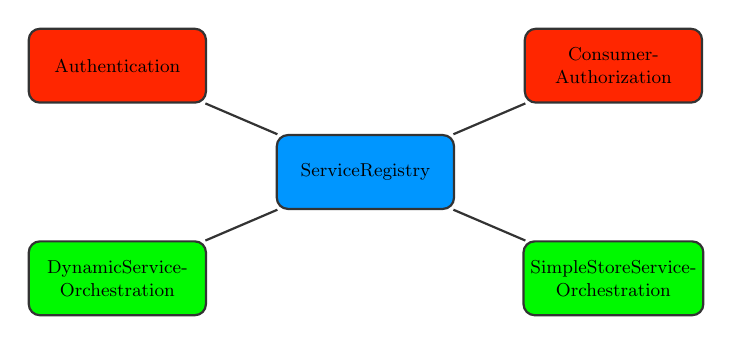
\begin{tikzpicture}[scale=0.75, every node/.style={transform shape}]
    \node[sr, ahRegistry] (sr) at (0,0) {ServiceRegistry};
    \node[authn, ahAuthentication] (an) at (-4.2,1.8) {Authentication};
    \node[authz, ahAuthorization] (az) at (4.2,1.8) {Consumer-\\Authorization};
    \node[orch, ahOrchestration] (do) at (-4.2,-1.8) {DynamicService-\\Orchestration};
    \node[orch, ahOrchestration] (so) at (4.2,-1.8) {SimpleStoreService-\\Orchestration};
    \foreach \n in {an,az,do,so} \draw[wire] (\n) -- (sr);
  \end{tikzpicture}

  \vspace*{\fill}

  \begin{abstract}
    This document outlines the 5th generation of the Arrowhead Core and Support systems as
    realised at the release candidate 5.3.0. The Core systems offer functionality expected to be needed for the
    majority of use cases where Arrowhead is applied: discovery, authentication, authorisation and
    orchestration. The Support systems offer functionality that many, but not all, deployments
    need: orchestration support, engineering and automation, credential life cycle, events, data,
    time, configuration, monitoring and inter-cloud connectivity. The document contains a
    high-level architectural description of what problems these systems solve and how they
    interact, including the management layer formed by the PlantDescriptionEngine and its
    engineering user interface, and the security mechanisms of the framework, to which the
    Onboarding system adds controlled admission of devices and
    systems. The blackbox descriptions of each core and support system
    is further detailed in their SysD and SD documents located in each system repository.

    The primary purpose of the document is to present the foundational
    architectural aspects thus necessary and often needed core and
    support systems. Implementation specifications are described
    in the white box GSoSDD documents \cite{gsosddcore,gsosddsup} and
    the core and support system SysDD
    and IDD documents for implementation detail located in each system repository.. The document supersedes \emph{GSoSD Arrowhead
    Core Systems 5.0 v1.2} \cite{gsosd50} and the draft \emph{GSoSD Arrowhead Support Systems 5.0}
    \cite{gsosdsup50}.
  \end{abstract}

  \vspace*{0.6cm}
\end{center}

\newpage
\tableofcontents
\newpage

%% ============================================================================================
\section{Overview}
\label{sec:overview}

This SoSD blackbox document provides the foundational Eclipse
Arrowhead framework architecture enabling the creation of technology
and engineering platforms for any application domain solution.

\paragraph{Graphics colour convention.}
All diagrams registry blue, authentication
and authorization red-orange, orchestration green, support yellow and application
orange. Both orchestration implementations share 
green; infrastructure is grey and mixed-system groups are neutral. These colours
identify roles rather than implementation languages. Turquoise is
reserved for service-interface elements. The SysML v1.6 Papyrus library's system-role fills, taken from
\prop{EclipseArrowhead-5.0/Arrowhead-5.0.notation} provides further
color details.
\begin{center}\scriptsize
\setlength{\fboxsep}{4pt}
\colorbox{AHSysMLRegistry}{\strut ServiceRegistry}\quad
\colorbox{AHSysMLSecurity}{\strut Authentication / ConsumerAuthorization}\\[6pt]
\colorbox{AHSysMLOrchestration}{\strut DSO / SimpleStore orchestration}\quad
\colorbox{AHSysMLSupport}{\strut Support}\quad
\colorbox{AHSysMLApplication}{\strut Application}\quad
\colorbox{AHSysMLInfrastructure}{\strut Infrastructure}
\end{center}

% \paragraph{Graphics colour convention.}
All diagrams use the SysML v1.6 Papyrus library's system-role fills, taken from
\prop{EclipseArrowhead-5.0/Arrowhead-5.0.notation}: registry blue, authentication
and authorisation red-orange, orchestration green, support yellow and application
orange. Both orchestration implementations share the library's combined-cloud
green; infrastructure is grey and mixed-system groups are neutral. These colours
identify roles rather than implementation languages. The library's turquoise is
reserved for service-interface elements.
\begin{center}\scriptsize
\setlength{\fboxsep}{4pt}
\colorbox{AHSysMLRegistry}{\strut ServiceRegistry}\quad
\colorbox{AHSysMLSecurity}{\strut Authentication / ConsumerAuthorization}\\[6pt]
\colorbox{AHSysMLOrchestration}{\strut DSO / SimpleStore orchestration}\quad
\colorbox{AHSysMLSupport}{\strut Support}\quad
\colorbox{AHSysMLApplication}{\strut Application}\quad
\colorbox{AHSysMLInfrastructure}{\strut Infrastructure}
\end{center}
%\input{sysml-color-legend.tex}
%\input{sysml-color-palette.tex}

%\paragraph{Graphics colour convention.}
All diagrams use the SysML v1.6 Papyrus library's system-role fills, taken from
\prop{EclipseArrowhead-5.0/Arrowhead-5.0.notation}: registry blue, authentication
and authorisation red-orange, orchestration green, support yellow and application
orange. Both orchestration implementations share the library's combined-cloud
green; infrastructure is grey and mixed-system groups are neutral. These colours
identify roles rather than implementation languages. The library's turquoise is
reserved for service-interface elements.
\begin{center}\scriptsize
\setlength{\fboxsep}{4pt}
\colorbox{AHSysMLRegistry}{\strut ServiceRegistry}\quad
\colorbox{AHSysMLSecurity}{\strut Authentication / ConsumerAuthorization}\\[6pt]
\colorbox{AHSysMLOrchestration}{\strut DSO / SimpleStore orchestration}\quad
\colorbox{AHSysMLSupport}{\strut Support}\quad
\colorbox{AHSysMLApplication}{\strut Application}\quad
\colorbox{AHSysMLInfrastructure}{\strut Infrastructure}
\end{center}
%\input{sysml-color-legend.tex}
%\input{sysml-color-palette.tex}


% \subsection{Implementation baseline and roadmap status (30 October 2026)}
% \label{sec:baseline-20261030}
% The architecture is realised by three primary source distributions:
% \prop{Eclipse-Arrowhead-java}, \prop{Eclipse-Arrowhead-go} and
% \prop{Eclipse-Arrowhead-rust}, under the Eclipse workspace. These are the
% sources for subsequent implementation changes; older \prop{Arrowhead/} and
% \prop{EA-fork/} checkouts are historical references or deployment consumers.
% A primary-source designation does not imply that every running image has been
% rebuilt from that tree. Release v5.2.2, local extensions, independently packaged
% sources and dated deployment evidence remain distinct \cite{primaryBaseline20261030}.

% \begin{table}[htbp]
% \centering\small
% \begin{tabularx}{\textwidth}{|P{1.6cm}|X|X|}\hline
% \rowcolor{gray!20} Language & Current source/build boundary & Evidence and limits \\\hline
% Java & Five core systems in \prop{ah5-core-java-spring}; fifteen independent
% support projects with own JAR/image/configuration. The Java-cloud manager is
% Node.js/nginx, despite its folder name. & Support packaging verified on
% 25 October; core/support services and operations tools have separate lifecycles.
% No shared JavaSupportRuntime dependency in the fifteen standalone projects. \\\hline
% Go & Five independent core modules and eighteen current top-level support/test/tool
% modules; private helper copies and optional \prop{go.work}. & 28 October audit:
% 22 module builds, tests and vet checks passed. Packaging does not establish
% complete Java parity or a new live rollout. \\\hline
% Rust & Five core entry points; fifteen support entry points and a separate
% LocalCloudManager crate in one Cargo workspace. Core/support libraries and
% messaging remain shared build dependencies. & 28 October copy report:
% 147 workspace tests passed. Per-system folders are not independently copied
% source closures. Java-equivalence and operational qualification remain open. \\\hline
% \end{tabularx}
% \caption{Current implementation structure, not a language-equivalence claim.
% Dated evidence is retained in each primary distribution
% \cite{javaPackaging20261025,goPackaging20261028,rustPackaging20261028}.}
% \end{table}
% \FloatBarrier

% \paragraph{Core inventory versus default cloud.}
% Five core implementations remain available. A \emph{new Java local-cloud design}
% selects ServiceRegistry, Authentication, ConsumerAuthorization and
% DynamicServiceOrchestration. SimpleStoreServiceOrchestration (labelled
% SimpleOrchestration by the configurator) is optional and absent from that default;
% it has not been deleted or implicitly stopped in an existing cloud. This is a
% configuration default, not a removal of the simple-store architecture or a new
% upstream release requirement \cite{javaLocalCloud20261030}.

% \paragraph{Database ownership and access boundary.}
% Every defined database is an \emph{integrated asset of its owning microsystem},
% including a separately deployed SQL or graph-database container. It is not
% selectable shared infrastructure or an independent service provider. Only host
% internal actions or services produced/consumed by that host mediate data access.
% The ownership rule also applies to embedded SQLite and private snapshot files.
% Brokers, relays and the constrained Docker proxy remain infrastructure. The
% Java catalog implements this rule for all sixteen defined database services;
% the default canvas therefore contains four microsystems, each with its own
% database, and one AMQP broker. The database assets do not become extra graph
% nodes \cite{javaDatabaseAssets20261030}.

% \begin{figure}[htbp]
% \centering
% % Current Java default design: owned assets are nested inside host boundaries.
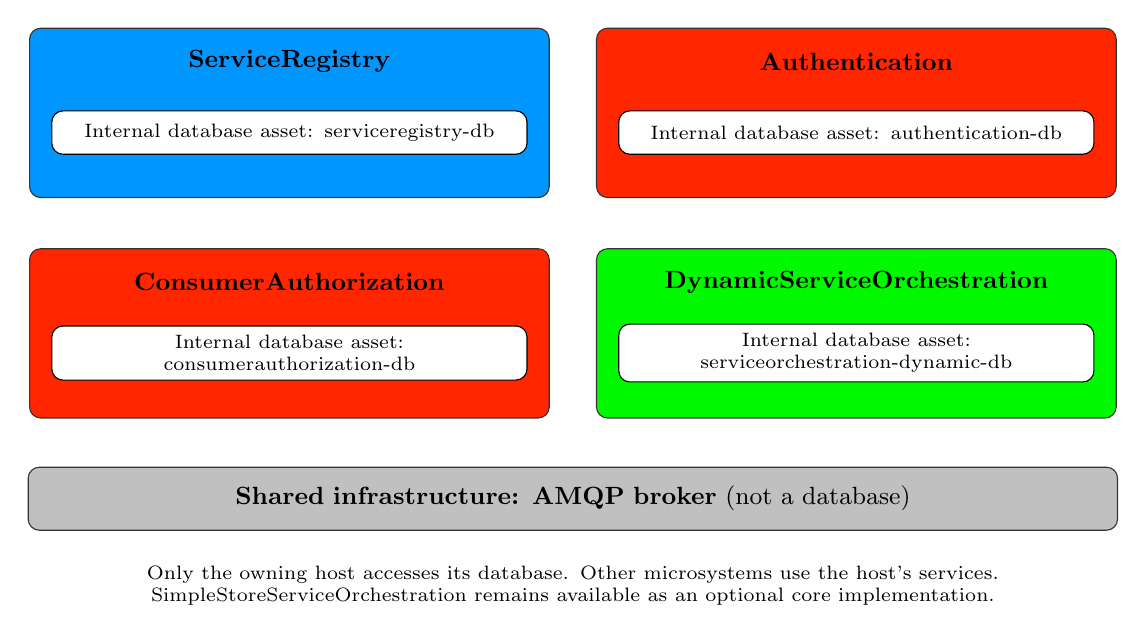
\begin{tikzpicture}[x=1cm,y=1cm,font=\small,
 host/.style={draw,rounded corners,minimum width=6.6cm,minimum height=2.15cm},
 asset/.style={draw,fill=white,rounded corners,text width=5.8cm,align=center,font=\scriptsize,minimum height=0.55cm}]
\node[host,ahRegistry] (sr) at (0,0) {};
\node at (0,0.65) {\textbf{ServiceRegistry}};
\node[asset] at (0,-0.25) {Internal database asset: serviceregistry-db};
\node[host,ahAuthentication] (auth) at (7.2,0) {};
\node at (7.2,0.65) {\textbf{Authentication}};
\node[asset] at (7.2,-0.25) {Internal database asset: authentication-db};
\node[host,ahAuthorization] (ca) at (0,-2.8) {};
\node at (0,-2.15) {\textbf{ConsumerAuthorization}};
\node[asset] at (0,-3.05) {Internal database asset: consumerauthorization-db};
\node[host,ahOrchestration] (dso) at (7.2,-2.8) {};
\node at (7.2,-2.15) {\textbf{DynamicServiceOrchestration}};
\node[asset] at (7.2,-3.05) {Internal database asset: serviceorchestration-dynamic-db};
\node[draw,rounded corners,ahInfrastructure,text width=13.6cm,align=center,minimum height=0.8cm] at (3.6,-4.9)
 {\textbf{Shared infrastructure: AMQP broker} (not a database)};
\node[text width=13.6cm,align=center,font=\scriptsize] at (3.6,-6.0)
 {Only the owning host accesses its database. Other microsystems use the host's services.\\
 SimpleStoreServiceOrchestration remains available as an optional core implementation.};
\end{tikzpicture}

% \caption{New Java default design. Each database is nested inside its owning
% microsystem boundary; it is not shared infrastructure or an independently
% selectable component. Colors retain the established Arrowhead system roles.}
% \label{fig:default-owned-assets}
% \end{figure}
% \FloatBarrier

% \paragraph{Evidence-qualified roadmap.}
% Recorded 19--24 October interoperability and federation results below remain
% historical acceptance of the stated workloads. The 23 October operation-count
% audit has not been replaced by a new complete differential audit. The Go
% packaging audit records a failing optional native-registry integration test:
% orchestration service registration is rejected, including with unmodified
% reference sources. Rust still has partial DTO/error/side-effect coverage,
% unsupported integrations and no automatic Java-state import. Complete
% replacement requires contract, policy, persistence and mixed-cloud acceptance
% for the exact image/configuration, beyond successful packaging tests
% \cite{goPackaging20261028,rustPackaging20261028,nativeCompatibility20261024}.

% \subsection{Graphical configuration and operational boundaries}
% \label{sec:configuration-update}
% The Java LocalCloudManager now offers three related engineering functions.
% Local-cloud composition selects microsystems and necessary infrastructure,
% stores named graphical designs, reviews the resulting actions and applies a
% confirmed deployment workflow. Its SoS view edits systems, service ports,
% connections and included SoS descriptions through PlantDescriptionEngine;
% activation is explicit and the PDE remains authoritative. The orchestration
% view edits local routing rules and ConsumerAuthorization policies graphically.
% Display positions are presentation data, not authorization grants.

% LocalCloudConfigurator configures one cloud; SoSConfigurator instead plans
% catalogued inter-cloud exchanges and their neighbour/policy changes. Both are
% operations tools using ColonyOS executors. They are not additional Arrowhead
% core systems and do not automatically register a discovery identity. An operator
% must review the plan before applying it. Saving a design does not change running
% systems; absence from a design does not implicitly stop an existing system
% \cite{javaLocalCloud20261030,javaSoS20261030}.

% The 30 October Java deployment inspection found 44 running containers in
% \prop{arrowhead-v52-test-cloud}: 23 microsystem processes, sixteen integrated
% database containers, two brokers, the manager UI, the Docker proxy and the
% LocalCloudConfigurator API. The microsystem count includes the optional
% GraphDBManager extension and Python demonstration producer; the manager API is
% counted once. GraphDBManager has no implementation in the supplied primary Java,
% Go or Rust source inventory; its existing Java-cloud image is a deployment
% extension, not evidence of a new portable support implementation. The older
% 22-system/41-container figure below is explicitly the 24 October snapshot
% \cite{roadmapInspection20261030}.


\section{Architecture fundamentals}

The Eclipse Arrowhead project provides a SOA/microservice architecture infrastructure enabling
the creation of an implementation platform for a certain application domain. This platform
facilitates the implementation of end-user solutions, as depicted in Figure~\ref{fig:concept}.

\begin{figure}[h!]
\centering
\begin{tikzpicture}[scale=0.8, every node/.style={transform shape}]
  \node[big, ahMixed] (ea) at (0,0) {Eclipse Arrowhead};
  \node[big, ahMixed] (soa) at (7,0) {SOA Architecture\\Infrastructure};
  \node[big, ahMixed] (ip) at (7,-2.5) {Integration Platform};
  \node[big, ahMixed] (si) at (7,-5) {Solution Implementation};
  \node[align=left, font=\normalsize, anchor=north west] at (-2.3,-0.9) {Infrastructure for distributed\\and modularised solutions\\from edge to cloud};
  \draw[-{Triangle[length=6mm,width=12mm]}, line width=6mm, ArrowheadBlue] (ea.east) -- (soa.west);
  \draw[-{Triangle[length=5mm,width=11mm]}, line width=5mm, orange] (soa.south) -- (ip.north);
  \draw[-{Triangle[length=5mm,width=11mm]}, line width=5mm, green!50!black] (ip.south) -- (si.north);
\end{tikzpicture}
\caption{Eclipse Arrowhead as SOA architecture infrastructure for integration platforms and
solution implementations.}
\label{fig:concept}
\end{figure}

The focus of Eclipse Arrowhead is microsystems that produce and consume microservices at the
edge. The Eclipse Arrowhead architecture and reference implementations target deployment on
heterogeneous devices from deep edge to fog, with interoperability to cloud microservices.

The Eclipse Arrowhead project exists to provide solutions and specifications that support
industrial and societal automation solutions that can adapt quickly and automatically to
changing circumstances and business requirements. This adaptability is enabled through
Service-Oriented Architecture (SOA), which entails dividing automation systems into smaller
independent systems that communicate by sending messages to, or consuming, the services
offered by the other systems. Each system is expected to be designed around the principles of
\begin{itemize}
  \item \textbf{loose coupling}, which means that services have narrow, well-defined application
        areas and depend internally on as few other services as possible to fulfil their
        functions,
  \item \textbf{late binding}, which entails providing as much functionality as possible given
        what needed services, configuration data and other details are currently available, as
        well as
  \item \textbf{lookup}, which means that systems, when possible, look up needed data by
        consuming services instead of relying on the data being in given configuration files.
\end{itemize}
These principles help facilitate the design of automation systems that are cheap and easy to
implement, upgrade, extend and reuse, are highly resilient to failures and attacks, and are
highly transparent about their constituents and activities.

While designing industrial automation systems around these principles has the advantages
mentioned, it also introduces the complexity inherent to all distributed applications. The
Core microsystems of Eclipse Arrowhead exist to help manage this complexity by facilitating
\begin{itemize}
  \item \textbf{discovery}, or helping microsystems independently find the services they need,
  \item \textbf{authentication}, or establishing the identity of the microsystems involved,
  \item \textbf{authorisation}, or regulating how microsystems are allowed to consume what
    microservices,
  \textcolor{blue}{\item \textbf{audit}, or means of keeping track of state,
    behavior and security over time,}  as well as
  \item \textbf{orchestration}, or centrally managing what microsystems consume what
        microservices.
\end{itemize}
Each of these concerns \textcolor{blue}{(except audit)} is addressed
by its own microservices, provided by its own microsystem, as outlined in the component diagram of
Figure~\ref{fig:component}. \textcolor{blue}{Audit is addressed by the introduction of
two services \svc{generalManagement} and svc{sysMonitor}
produced by all v5.3 core and support system, with a strong recommendation
to be produced by all application system.} Further concerns that are common
but not universal -- such as engineering-driven orchestration, workflows, credential life cycle,
events, data, time, configuration, monitoring and inter-cloud connectivity -- are addressed by the
Support microsystems.

\begin{figure}[h!]
\centering
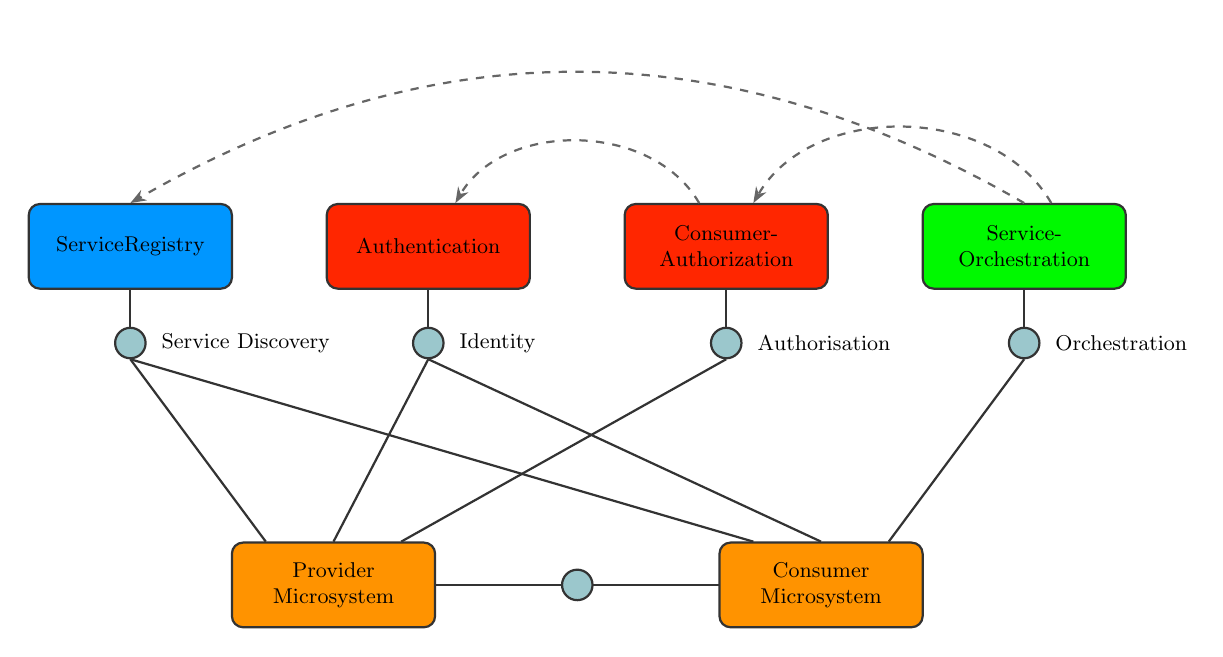
\begin{tikzpicture}[scale=0.86, every node/.style={transform shape}]
  \node[sr, ahRegistry]    (sr) at (0,0)     {ServiceRegistry};
  \node[authn, ahAuthentication] (an) at (4.4,0)   {Authentication};
  \node[authz, ahAuthorization] (az) at (8.8,0)   {Consumer-\\Authorization};
  \node[orch, ahOrchestration]  (or) at (13.2,0)  {Service-\\Orchestration};
  \node[app]   (pr) at (3.0,-5.0) {Provider\\Microsystem};
  \node[app]   (co) at (10.2,-5.0) {Consumer\\Microsystem};
  % provided interfaces (lollipops)
  \foreach \n/\l in {sr/Service Discovery, an/Identity, az/Authorisation, or/Orchestration} {
    \draw[wire] (\n.south) -- ++(0,-0.55) node[lolli, anchor=north] (L\n) {};
    \node[font=\small, anchor=west] at ($(L\n.east)+(0.1,0)$) {\l};
  }
  \node[lolli] (Lpr) at (6.6,-5.0) {};
  \draw[wire] (pr.east) -- (Lpr.west);
  \draw[wire] (Lpr.east) -- (co.west);
  % consumption: each provided service to its consumers
  \draw[wire] (Lsr.south) -- ($(pr.north)+(-1.0,0)$);
  \draw[wire] (Lan.south) -- ($(pr.north)+(0,0)$);
  \draw[wire] (Laz.south) -- ($(pr.north)+(1.0,0)$);
  \draw[wire] (Lsr.south) -- ($(co.north)+(-1.0,0)$);
  \draw[wire] (Lan.south) -- ($(co.north)+(0,0)$);
  \draw[wire] (Lor.south) -- ($(co.north)+(1.0,0)$);
  % consumption between Core systems
  \draw[owire, -{Stealth[length=2mm]}] (or.north) to[out=150,in=30] (sr.north);
  \draw[owire, -{Stealth[length=2mm]}] ($(or.north)+(0.4,0)$) to[out=120,in=60] ($(az.north)+(0.4,0)$);
  \draw[owire, -{Stealth[length=2mm]}] ($(az.north)+(-0.4,0)$) to[out=120,in=60] ($(an.north)+(0.4,0)$);
\end{tikzpicture}
\caption{Core microsystems of a local cloud. Each box is a microsystem; a circle is a provided
microservice; solid lines show which application systems consume which Core services, dashed
arrows consumption between Core systems (registration of every system in the ServiceRegistry is
omitted). ServiceOrchestration stands for
either of the two orchestration microsystems of Section~\ref{sec:orch}.}
\label{fig:component}
\end{figure}

A deployment of microsystems interrelated in this manner makes up a System-of-Systems (SoS).
When a System-of-Systems can fulfil its core functionality without external support, we refer
to it as a \emph{local cloud}. Local clouds enable the segmentation of complex SoS. Such
segmentation results in multiple local clouds which can interact with each other; such a
system of multiple local clouds is referred to as a \emph{system of local clouds}.

Microservices shall be referenced by their microservice type, i.e.\ their \emph{service
definition}. Since release 5.2 the names of microsystems, microservices, operations and
interface templates follow the agreed naming convention \cite{naming2}
(Section~\ref{sec:nfr:naming}).

In Section~\ref{sec:microsystems} we consider what the Core services and systems do in more
detail, and in Section~\ref{sec:support} the Support systems. Section~\ref{sec:mgmtsec}
describes the management layer and the security mechanisms of the framework. In
Section~\ref{sec:usecases} we
describe use cases in which some or all of them are used. In Section~\ref{sec:planes} we discuss
how Core and Support systems relate to the control and data planes of a distributed application.
In Section~\ref{sec:release} we outline the differences between
Arrowhead 4.x, 5.0, 5.2.2 and 5.3. In
Section~\ref{sec:nfr} we present key non-functional requirements, and in
Section~\ref{sec:issues} the issues that are currently open. Finally,
Sections~\ref{sec:refs} and \ref{sec:history} list references and versions.
Appendix~\ref{app:matrix} contains the system-service matrix.

\newpage
%% ============================================================================================

\subsection{Non-Functional Requirements}
\label{sec:nfr}

Setting up and operating an Arrowhead local cloud comes with the caveats shared by all
distributed systems. Managing them typically means prioritising certain qualities when
designing or choosing the systems for a local cloud. This section outlines the qualities
promoted by the Eclipse Arrowhead project as non-functional requirements.

\subsubsection{Accurate Enough Message Caching}
\label{sec:nfr:cache}
Most modern computing devices, including embedded ones, can call local functions in the order of
microseconds or faster. In contrast, calling a function on another device by sending a message
typically takes milliseconds or longer. The relative expense, in time and capacity, of sending
messages is often high enough to make it worthwhile to reduce the number of messages that must be
sent for the use case at hand.

One important way to reduce messaging is to let systems cache data they receive. When a system
needs some data, it first consults its cache; if it finds the data there, no message needs to be
sent. The trade-off is that cache entries become invalid as soon as the original data change.
Unless the caching systems are notified, they cannot be confident the data has not changed
without requesting it again. If notification is impractical, cache entries can be expired when
too old or when other factors suggest they may be invalid.

Caching can thus reduce messaging, but using it requires planning how to avoid systems acting on
invalid entries. The Arrowhead Core and Support systems must be designed to make it easy to reason
about and manage the caching of the data they hold. In 5.2.2 this is supported by expiry times on
registry entries, time-limited identity and access tokens, self-contained tokens that can be
verified without contacting their issuer, short-lived caching of authorisation decisions in
providers, and push orchestration, which notifies consumers of changes. Among the Support systems,
the \sys{DataManager} proxy serves cached values on behalf of producers, the \sys{SysMonitor} keeps a
history so that consumers need not query each monitored system, and systems may cache their
configuration and the trusted time between fetches.

\subsubsection{Relative System Independence}
Systems tend to become more brittle the larger and more complicated they become, and local
clouds are no exception: the more and the more complicated the systems of a local cloud, the
higher the probability that one of them degrades or breaks. This can be mitigated by systems with
small scopes, so that fewer things can break in each, and by making systems able to work around
such eventualities independently. Independence means that each system needs to own enough
resources and capabilities, which among other things entails systems owning their own data
rather than storing it in shared external databases. Every 5.2.2 Core and Support system owns
its data store.

Designing a local cloud effectively means that its resilience to failures must be accounted for,
and that its systems are given the capabilities required to work around contingencies.

\subsubsection{Backwards Compatibility}
\label{sec:nfr:compat}
For major releases some backwards incompatibility may occur. From 4.x.y to 5.0.0 the Core and
Support systems became responsible for their own data; 4.x.y used a common SQL database, which is
not the case for 5.0.0 onwards. 5.x.y Core systems are therefore not backwards compatible with
4.6.1 and its predecessors. The general approach to backwards compatibility follows these
guidelines:
\begin{itemize}
  \item A 5.$x$+1.$y$ release is based on a new Core system being added or a major update of one
        of the released Core systems. A 5.$x$.$y$+1 release contains bug fixes.
  \item 4.6.1 is maintained for at least 12 months after the release of 5.0.0.
  \item 5.1 shall be backwards compatible with 5.0; 5.2 with 5.0 and 5.1; 5.3 with 5.0, 5.1 and
        5.2.
\end{itemize}
Migrated 4.6 Support systems keep their 4.6 URL paths and ports where possible but are not wire
compatible with 4.6 clients, since identities, payloads and management interfaces follow 5.x.

\subsubsection{Authentication Mechanisms}
Eclipse Arrowhead has the ambition to support a number of authentication mechanisms. For 5.x the
major approach is X.509 certificates following the Arrowhead certificate profile. Release 5.2.2
adds identity tokens issued by the \sys{Authentication} system, and the combination of both.
Self-declared identities exist for development only. With the \sys{Onboarding} system, the
certificates and identities themselves are issued through a controlled procedure that starts from
a manufacturer bootstrap certificate approved by an operator (Section~\ref{sec:secmech}). Further mechanisms such as OpenID Connect
and OAuth will be investigated and decided upon in due course.

\subsubsection{Naming Convention for Local Clouds, Microsystems, Microservices, \ldots}
\label{sec:nfr:naming}
A naming convention has been agreed by the Roadmap WG \cite{naming2}; the earlier proposal by
Cristina Paniagua and Jerker Delsing from 2019 was considered too complex. Release 5.2.2 applies
it as follows:

\begin{table}[h!]
\centering\footnotesize
\begin{tabularx}{\textwidth}{|P{4.4cm}|P{4.6cm}|Y|}\hline
\rowcolor{gray!33}Identifier & Form & Example \\\hline
Microsystem (system name) & PascalCase, ASCII letters and digits & \prop{DynamicServiceOrchestration} \\\hline
Microservice (service definition) & camelCase, ASCII letters and digits & \prop{serviceOrchestration} \\\hline
Service operation & lowercase kebab-case & \prop{modify-priorities} \\\hline
Interface template & lowercase snake\_case & \prop{generic_mqtts} \\\hline
\end{tabularx}
\caption{Naming convention as applied in 5.2.2.}
\label{tab:naming}
\end{table}

Deployment identifiers -- software packages, URL paths, container and host names, database names
-- keep the forms required by their platforms and are not Arrowhead system or service names.

\subsubsection{Active vs.\ Passive Systems}
The Arrowhead Core Framework supports both active and passive systems.
\begin{description}
  \item[Active systems] act on their own behalf and can at any time change consumed or produced
        services. They interact with the Core Framework to obtain the information they need,
        typically by pull orchestration.
  \item[Passive systems] normally wait for some external stimulus before acting. They perform
        their duty and then return to a waiting state. Push orchestration lets the Core Framework
        deliver the stimulus.
\end{description}
\emph{Consequences for the Core Framework}: it must support systems ranging from very passive to
fully active, and it must be resilient to systems that make their own decisions in terms of,
for example, authorisation and orchestration.

\subsubsection{Port Numbering}
\label{sec:nfr:ports}
Systems find each other through the \sys{ServiceRegistry}, so only its port must be known for
bootstrapping. Well-known default ports nevertheless matter for co-location, firewalls and
running several local clouds side by side. The following rules apply; the complete
specification and allocation table are given in the Core GSoSDD \cite{gsosddcore}.
\begin{itemize}
  \item Every Arrowhead framework system type has one canonical port, unique across the
        framework and used for all its HTTP(S) services; allocated ports are stable, and ports of
        retired systems remain reserved.
  \item A local cloud uses the port block 8000--8999, divided into ranges: tunnel control pool
        (8000--8099), inter-cloud session endpoints (8200--8299), life-cycle and engineering
        systems (8430s), Core and trust systems (8440s; \sys{ServiceRegistry} 8443), support
        systems (8450--8469), monitoring and QoS (8470s), health endpoints (8480s), operator tools
        (8490s), application systems (8500--8799) and messaging (8883 MQTT over TLS). The AMQP
        broker for \svc{sysMonitor} uses the well-known AMQP-over-TLS port 5671. The inter-cloud
        relay is organisation infrastructure outside the blocks of the local clouds.
  \item Local clouds sharing hosts or addresses in a system of local clouds are given a cloud
        index $k \in \{0,\ldots,23\}$ and use port $=$ canonical $+\,1000\cdot k$, which keeps all
        ports below the ephemeral range.
\end{itemize}

\newpage
%% ============================================================================================
\section{Core Microsystems}
\label{sec:microsystems}

The Core systems of the Eclipse Arrowhead project address concerns expected to be typical of
most settings where SOA is applied. We describe them here in the abstract. Release 5.2.2
provides five Core microsystems; their mandatory and optional status in a local cloud and
their microservices are listed in Table~\ref{tab:core}. Full AA and encrypted
communication are the default from v5.0; optional orchestration or Support features
do not make authentication or authorisation optional.

\begin{table}[h!]
\centering\footnotesize
\begin{tabularx}{\textwidth}{|P{4.0cm}|P{1.9cm}|P{4.8cm}|Y|}\hline
\rowcolor{gray!33}Microsystem & Status & Microservice & Purpose \\\hline
\multirow{4}{*}{\parbox{3.9cm}{\sys{ServiceRegistry}}} & \multirow{4}{*}{mandatory}
 & \svc{serviceDiscovery} & Register, look up and revoke service instances \\\cline{3-4}
 & & \svc{systemDiscovery} & Register, look up and revoke systems \\\cline{3-4}
 & & \svc{deviceDiscovery} & Register, look up and revoke devices \\\cline{3-4}
 & & \svc{serviceRegistryManagement} & Bulk administration of all registry content \\\hline
\multirow{2}{*}{\sys{Authentication}} & \multirow{2}{*}{mandatory}
 & \svc{identity} & Log in, log out, change credentials, verify identities \\\cline{3-4}
 & & \svc{identityManagement} & Administration of identities and sessions \\\hline
\multirow{4}{*}{\sys{ConsumerAuthorization}} & \multirow{4}{*}{mandatory}
 & \svc{authorization} & Grant, revoke, look up and verify access rules \\\cline{3-4}
 & & \svc{authorizationToken} & Generate and verify access tokens \\\cline{3-4}
 & & \svc{authorizationManagement} & Administration of access rules \\\cline{3-4}
 & & \svc{authorizationTokenManagement} & Administration of tokens and encryption keys \\\hline
\multirow{4}{*}{\parbox{3.9cm}{\sys{DynamicService-}\\\sys{Orchestration}}} & \multirow{4}{*}{\parbox{1.8cm}{optional, one of the two}}
 & \svc{serviceOrchestration} & Orchestration pull and push (subscribe, unsubscribe) \\\cline{3-4}
 & & \svc{serviceOrchestrationPushManagement} & Administration of push subscriptions \\\cline{3-4}
 & & \svc{serviceOrchestrationLockManagement} & Administration of exclusivity locks \\\cline{3-4}
 & & \svc{serviceOrchestrationHistoryManagement} & Orchestration history \\\hline
\multirow{4}{*}{\parbox{3.9cm}{\sys{SimpleStoreService-}\\\sys{Orchestration}}} & \multirow{4}{*}{\parbox{1.8cm}{optional, one of the two}}
 & \svc{serviceOrchestration} & Orchestration pull and push (same interface) \\\cline{3-4}
 & & \svc{serviceOrchestrationSimpleStoreManagement} & Administration of orchestration rules \\\cline{3-4}
 & & \svc{serviceOrchestrationPushManagement} & Administration of push subscriptions \\\cline{3-4}
 & & \svc{serviceOrchestrationHistoryManagement} & Orchestration history \\\hline
All Core systems & -- & \svc{generalManagement} & Logs and configuration of the system \\\hline
\end{tabularx}
\caption{Core microsystems and microservices of release 5.2.2 under the default
v5.0-and-later AA security baseline. Orchestration strategy remains a deployment choice.}
\label{tab:core}
\end{table}

The purposes of the respective Core systems are presented in Section~\ref{sec:sysdesc}. In
Section~\ref{sec:bootstrap} we consider how local clouds reach a working state from a cold start,
and in Section~\ref{sec:matrix} we introduce the system-service matrix of Core and Support
systems.

In addition to the Core systems, several \emph{Support} systems are provided. We expect them to
be common in many Arrowhead deployments, but since they are not as essential as the Core systems,
they are described separately in Section~\ref{sec:support}. Three of them are invoked by the
advanced Orchestration system.

%% --------------------------------------------------------------------------------------------
\subsection{System Descriptions}
\label{sec:sysdesc}

We now state the purposes and services of the Core systems informally. More detailed
descriptions of the services are given in the Service Descriptions (SDs), their realisations
in the Interface Design Descriptions (IDDs), and the internal design of the 5.2.2 systems in
the white-box GSoSDD \cite{gsosddcore}.

\subsubsection{ServiceRegistry}
\label{sec:sr}
One of the main principles of SOA is lookup: whenever possible, data required for whatever
reason should be looked up by consuming a service. One kind of data that is virtually always
required to facilitate a system-of-systems is the network information, such as addresses and
port numbers, needed by systems to communicate with each other.

The \sys{ServiceRegistry} holds the registry of the local cloud. It maps the identifiers of
individual service instances to the information generally required to communicate with their
providers. Since 5.x the registry also records the \emph{systems} that provide services and the
\emph{devices} that host systems, so that the physical deployment of the local cloud can be
expressed and queried. A service instance is identified by its provider system, service
definition and version; each instance has one or more \emph{interfaces}, each an instance of an
\emph{interface template} (for example HTTPS or MQTTS in the default secure profile) that defines which interface
properties must be given. Each interface also states the \emph{security policy} a consumer must
satisfy, such as certificate-based access or a particular kind of access token.

Individual systems register, update or revoke their own devices, systems and services through
the \svc{deviceDiscovery}, \svc{systemDiscovery} and \svc{serviceDiscovery} services, and other
systems look them up through the same services. Alternatively, the registry can be populated by
an operator through the \svc{serviceRegistryManagement} service, which allows registry content
to be created, updated, removed and queried in bulk and is meant primarily for administration.

When using a \sys{ServiceRegistry}, the only network address systems are required to know is
that of the \sys{ServiceRegistry}. With that, systems can look up the network addresses of the
systems they need to consume, given that they know their service definitions or instance
identifiers. Entries are not limited to network details: they may include metadata relevant
for selecting service instances, such as the physical location of temperature sensors or the
conveyor belt at which a welding service is provided. Lookups can filter on metadata.

A local cloud may \emph{restrict} direct discovery. In restricted mode, ordinary systems can only
discover the public Core services directly (those marked for unrestricted discovery, such as
\svc{identity}, \svc{authorization} and \svc{serviceOrchestration}); all other services must be
obtained through orchestration, which applies authorisation. Systems that need to search the
whole registry, such as the orchestration system, are granted direct access by configuration.
Atomic orchestration returns only service-instance identifiers, so in restricted mode a
consumer that resolves them must also be granted direct access. Advanced orchestration needs
no such grant, because its results carry the access information.

\subsubsection{Authentication System}
\label{sec:authn}
In order to enable authorisation to fulfil its purpose in a secure manner, the systems that
consume services must be properly identified. The \sys{Authentication} system provides the identity service used by the default
AA architecture. Certificate-based peer authentication and identity tokens are
complementary mechanisms in the secure reference profile. Identities can be set at
deployment time, for example as an X.509 certificate following the Arrowhead certificate
profile, or issued dynamically, for example in the form of a token. The \sys{Authentication}
system issues time-limited identity tokens after a successful login (\svc{identity}) and
validates them on behalf of other systems, so that systems are known to be the ones they claim
to be. Identities and their credentials are administered through \svc{identityManagement}.

The implementation supports the following identity mechanisms; only authenticated
mechanisms are part of the default cloud profile:
\begin{itemize}
  \item \textbf{certificate} -- mutual TLS with Arrowhead-compliant X.509 certificates; the
        system name is taken from the certificate;
  \item \textbf{identity token} -- the system logs in to \sys{Authentication} and presents the
        token, which providers verify with \sys{Authentication};
  \item \textbf{self-declared} -- the system states its name; intended for development only.
        The Java reference refuses to start with it unless the development exception is
        selected explicitly.
\end{itemize}
The secure reference profile combines certificates and identity tokens: the token's
system name must match the authenticated certificate. A certificate-only service
binding must still enforce the applicable authorisation policy and encrypted transport. A limitation of Arrowhead 5.2.2 is that only \emph{system} authentication is
performed; user authentication is still under investigation (Section~\ref{sec:issues}).

\subsubsection{Authorisation System}
\label{sec:authz}
Authorisation is part of the default AA security baseline from v5.0. Every service
provider must establish which authenticated systems may consume its services and
operations, and under which limitations. The Authorisation system,
realised by \sys{ConsumerAuthorization}, holds access 
control rules (\emph{policies}) that state, for a provider and a service definition (or event
type), and optionally per operation, which consumers are permitted. A policy may permit all
consumers, a list of consumers (whitelist), all but a list (blacklist), or the consumers whose
system metadata satisfies a requirement. Whenever a system attempts to consume a service, the
provider enforces a positive authorisation decision, obtained through
\sys{ConsumerAuthorization} or a valid service-bound authorisation token, before
executing the operation.

Using an Authorisation system means that individual service providers do not need to know in
advance what other systems are allowed to consume them. Rules exist on two levels: a provider
may grant rules for its own services (provider level, \svc{authorization}), and the local cloud
operator manages rules for any service (management level, \svc{authorizationManagement}).
\textbf{Management-level authorisation rules have priority over the producing
application system's own rules}; if no rule applies, access is
denied.

\sys{ConsumerAuthorization} can also issue \emph{access tokens} (\svc{authorizationToken}): time-limited,
usage-limited and self-contained (signed, e.g.\ JSON Web Tokens) tokens bound to a consumer,
provider, service and operation. Self-contained tokens can be verified by the provider without
contacting \sys{ConsumerAuthorization}. Tokens and provider encryption keys are administered
through \svc{authorizationTokenManagement}. To reduce the number of times a system has to consult
the Authorisation system, caching may be employed, as discussed in Section~\ref{sec:nfr:cache}.

\subsubsection{Orchestration System}
\label{sec:orch}
Using only the \sys{ServiceRegistry} means that network information does not have to be
manually supplied to the individual systems of a local cloud. However, each system must still be
configured, or use its own search procedure, to determine what exact service instances to
consume. This becomes an issue when the same type of service is provided by many systems that
differ in other respects: if a service instance reports the air quality for a specific
location, which instance is consumed affects what data the consumer receives.

The main task of the Orchestration system is to help consumers decide which service instances
they should use. An orchestration request can result in a list of providers offering different
services (to satisfy all the consumer's needs), a list of providers offering the same service
(viable alternatives), or a single provider. In contexts where tokens are used for access
control, the Orchestration system also delivers these tokens together with the service
instances to consume.

There are two approaches to how an Orchestration system can fulfil this task, with different
advantages and disadvantages. Release 5.2.2 provides both, with a shared interface, and the
operator of the local cloud decides which kind of orchestration the local cloud uses:

\begin{description}
  \item[Atomic orchestration -- \sys{SimpleStoreServiceOrchestration}.] Holds a table of
        prioritised rules that map each consumer and service definition to the specific service
        instances it should consume. An orchestration request returns service instance
        identifiers in priority order; the consumer uses them to acquire access information from
        the \sys{ServiceRegistry}. This approach is very simple, uses few computing resources and
        does not perform the dynamic eligibility pipeline. Resolving a stored rule still
        requires secure discovery and provider-side authorisation; a rule is not an
        access grant. Its limitations are that most tasks are delegated to the consumer,
        that it issues no access tokens, and that
        keeping the rules consistent with the registry is a task for the operator or a support
        system (for example the \sys{PlantDescriptionEngine}).
  \item[Advanced orchestration -- \sys{DynamicServiceOrchestration}.] Computes the result at
        request time from the consumer's requirements (service definition, operations,
        interfaces, security policies, metadata, preferred providers, QoS requirements,
        exclusivity) and flags (matchmaking, only preferred, only exclusive, allow translation,
        allow or only inter-cloud). It uses ServiceRegistry and the default AA foundation;
        additional Support systems enable optional capabilities. Its functions include:
        \begin{itemize}
          \item \textbf{Authorisation}: providers the consumer is not authorised to use are
                removed from the response, and the necessary tokens are added automatically;
          \item \textbf{Exclusivity}: providers can be reserved (locked) for one consumer for a
                period of time;
          \item \textbf{Blacklist}: blacklisted providers are removed;
          \item \textbf{Translation}: if no compatible provider exists, a translation bridge
                between interfaces or data models is set up through the \sys{TranslationManager};
          \item \textbf{QoS}: providers are filtered or ranked by the quality of their devices
                (\sys{DeviceQoSEvaluator});
          \item \textbf{Inter-cloud}: orchestration across local clouds through
                \sys{Gatekeeper} and \sys{GateTunnel}.
        \end{itemize}
        It is more convenient for consumers, since the response contains everything needed to
        consume the service, but it is more complex, uses more computing resources and depends on
        other systems.
\end{description}

Consumers obtain their orchestration results by \emph{pull} (\op{pull} of
\svc{serviceOrchestration}) or subscribe to \emph{push} orchestration (\op{subscribe},
\op{unsubscribe}), in which case results are delivered to them when triggered. The orchestration
history, push subscriptions, locks and (for the atomic approach) the rule store are administered
through dedicated management services.

To address the late binding and loose coupling properties of SOA, orchestrating who
can/should/shall talk to whom is important. The orchestration system thus provides rules on who
can/should/shall talk to whom; these rules may be based on policies. Such rules can be
``owned'' by a consumer, a plant description microsystem, a workflow/choreography microsystem,
the orchestration microsystem, or an operator (engineering). The hierarchy developed in
Arrowhead is
\begin{enumerate}
  \item Operator -- engineering,
  \item PlantDescription,
  \item Orchestration,
  \item Consumer.
\end{enumerate}
For interoperability reasons both push and pull distribution of orchestration rules are
supported. Each local cloud has its own orchestration system. In principle there can be
multiple orchestration systems in a local cloud, but that creates synchronisation requirements;
the recommendation is therefore to have one orchestration system in a local cloud (see
Section~\ref{sec:issues} for a current exception).

Orchestration between local clouds is made possible by the \sys{Gatekeeper} and
\sys{GateTunnel} microsystems, in cooperation with the \sys{ServiceRegistry} and the
authentication and authorisation microsystems of the other local clouds.

It has to be noted that an application implementation where consumers are ``free'' to use their
``own orchestration'' information gives less understanding and control of what goes on in a
local cloud, with possible consequences for real-time, security and safety properties.
Unforeseen issues may thus emerge.


%% --------------------------------------------------------------------------------------------
\subsection{Local Cloud Bootstrapping}
\label{sec:bootstrap}

Since v5.0, full authentication and authorisation (AA) and encryption of exchanged
information are the default for an Arrowhead local cloud. Bootstrapping establishes
that protected operating state before ordinary service consumption begins. It does
not start an unsecured registry-only cloud and add security later. Discovery,
registration, identity exchange, policy administration, orchestration and application
traffic all remain subject to the default security baseline.

Before startup, every system has a unique Arrowhead identity, the credentials
needed to prove it, and the trust material needed to authenticate its peers.
Initial credentials and access policies are provisioned by the operator, or obtained
through an approved onboarding procedure. The ServiceRegistry bootstrap address
must be known or obtained through a trusted mechanism; learning an address does
not establish trust in the system at that address.

\begin{enumerate}
  \item \textbf{Establish trust and protected communication.} Provision the local-cloud
        trust anchors, system/operator credentials and the information needed to check
        their validity and revocation. Enable encrypted, integrity-protected transport
        with authenticated peers before exposing any Core endpoint. The reference
        deployment uses mutual TLS for HTTPS, AMQPS and MQTTS. Credentials and tokens
        are never exchanged over a plaintext bootstrap channel.
  \item \textbf{Start the ServiceRegistry as the discovery anchor.} It registers its
        own services and advertises protected interfaces. Systems may discover the
        Core endpoints needed to complete authentication and authorisation, but such
        bootstrap discovery is narrowly scoped and does not waive peer authentication,
        encryption or management protection.
  \item \textbf{Make AAA services ready.} Start Authentication and
        ConsumerAuthorization with their bootstrap identities, operator rights and
        initial policies. In the certificate-bound token profile, systems obtain an
        identity token over mutual TLS and providers verify its binding to the caller.
        Authorisation policies govern the provider, service and requested operation;
        missing permission or an unavailable required verification fails closed.
  \item \textbf{Enable authorised orchestration.} Start the selected orchestration
        implementation after its discovery and AAA dependencies are ready. SimpleStore
        uses provisioned consumer-to-service rules; dynamic orchestration evaluates
        each requirement against eligible, authorised providers. Selection does not
        remove the provider's responsibility to enforce access control.
  \item \textbf{Admit Support and application systems.} Each system authenticates,
        registers its protected service interfaces and consumes services only within
        its granted rights. Onboarding establishes credentials, not service permissions.
        Monitoring, management and any inter-cloud path follow the same AAA and
        confidentiality requirements. Support prerequisites are listed in
        Section~\ref{sec:sup:deploy}.
\end{enumerate}

These are readiness conditions, not permission to create an anonymous startup
window or a rigid process order that ignores implementation dependencies.
Bootstrap credentials and scoped policies must break dependency cycles without
bypassing AAA. Certificate authentication and certificate-bound identity tokens are
mechanisms for satisfying the baseline; self-declared names and unencrypted
HTTP/MQTT do not satisfy it. Any deliberately unsecured test setup is an explicit,
isolated development exception, not the default architecture. The Java reference
enforces this at startup: a system below the baseline stops before it opens a port,
unless the exception is selected explicitly \cite{javaConformance20261107}. A registry-only
example can illustrate lookup but is not a complete local-cloud deployment under
the v5.0-and-later security baseline.



\newpage
%% ============================================================================================
\section{Support Microsystems}
\label{sec:support}

The Core systems address concerns typical of every local cloud. \emph{Support} systems address
concerns that many, but not all, deployments have: richer orchestration, engineering-driven
configuration of the local cloud, workflow execution, the life cycle of credentials, events, data,
time, configuration, monitoring and connectivity between local clouds. Support systems are
optional; each is deployed when its concern is present. They behave like any other microsystem
of the local cloud: they register in the \sys{ServiceRegistry}, are identified by certificate or
identity token, are subject to the rules of the Authorisation system, and are found through
discovery or orchestration.

This section replaces the largely unwritten \emph{GSoSD Arrowhead Support Systems 5.0}
\cite{gsosdsup50}. It describes the Support systems in the abstract, as for the Core systems in
Section~\ref{sec:microsystems}; the white-box design of each 5.2 Support system is given in
\cite{gsosddsup}, and per-system SysD, SD and IDD documents are published with the
implementations.

\subsection{Overview and Release Status}
\label{sec:sup:overview}

Two groups of Support systems exist at the 5.2 level:
\begin{itemize}
  \item \textbf{Released with Eclipse Arrowhead 5.2.2} \cite{ah5supportup}: \sys{Blacklist},
        \sys{TranslationManager} and \sys{DeviceQoSEvaluator}. They extend the advanced
        Orchestration system.
  \item \textbf{Project implementations on the 5.2.2 baseline} \cite{ah5support}: twelve active support
        systems migrated from Arrowhead 4.6 or newly designed, deployed and verified in the 5.2.2
        test beds but not yet reviewed for an upstream release (Section~\ref{sec:issues}).
        Since 9~November~2026 every Core and support system of the Java reference implementation,
        including the operator tools LocalCloudManager, LocalCloudConfigurator and SoSConfigurator,
        is a Java-Spring system on the common Arrowhead library; contracts are unchanged.
        The former delegated SysMonitorPublisher is retained only as historical
        documentation, not a sixteenth active support implementation.
\end{itemize}

\begin{table}[h!]
\centering\footnotesize
\begin{tabularx}{\textwidth}{|P{2.6cm}|P{3.5cm}|P{5.4cm}|Y|}\hline
\rowcolor{gray!33}Area & Microsystem & Microservices & Purpose \\\hline
\multirow{3}{*}{\parbox{2.5cm}{Orchestration support}}
 & \sys{Blacklist}$^{U}$ & \svc{blacklistDiscovery}, \svc{blacklistManagement} & Exclude misbehaving systems from the local cloud \\\cline{2-4}
 & \sys{TranslationManager}$^{U}$ & \svc{translationBridge}, \svc{translationBridgeManagement}, \svc{translationReport} & Bridge incompatible interfaces and data models \\\cline{2-4}
 & \sys{DeviceQoSEvaluator}$^{U}$ & \svc{qualityEvaluation}, \svc{deviceQualityDataManagement} & Rank providers by the quality of their devices \\\hline
\multirow{3}{*}{\parbox{2.5cm}{Engineering \& automation}}
 & \sys{PlantDescriptionEngine} & \svc{plantDescriptionManagement}, \svc{plantDescriptionMonitor} & Derive orchestration rules from an engineered plant description; report deviations \\\cline{2-4}
 & \sys{Choreographer} & \svc{choreographerSession}, \svc{choreographerExecutor}, \svc{choreographerManagement} & Execute workflows on executor systems \\\cline{2-4}
 & \sys{Configuration} & \svc{configuration}, \svc{configurationProxy}, \svc{configurationManagement} & Distribute configuration files to systems \\\hline
\multirow{2}{*}{\parbox{2.5cm}{Security \& life cycle}}
 & \sys{CertificateAuthority} & \svc{certificateSigning}, \svc{certificateValidation}, \svc{certificateAuthorityManagement} & Issue, validate and revoke certificates \\\cline{2-4}
 & \sys{Onboarding} & \svc{onboarding}, \svc{onboardingManagement} & Admit (onboard) and withdraw (off-board) devices and their systems \\\hline
\multirow{3}{*}{\parbox{2.5cm}{Information \& messaging}}
 & \sys{EventHandler} & \svc{eventPublish}, \svc{eventSubscription}, \svc{eventHandlerManagement} & Publish/subscribe of events \\\cline{2-4}
 & \sys{DataManager} & \svc{dataProxy}, \svc{dataHistorian} & Cache and store sensor and actuator data \\\cline{2-4}
 & \sys{TimeManager} & \svc{time} & Trusted time for the local cloud \\\hline
\multirow{2}{*}{\parbox{2.5cm}{Monitoring \& analytics}}
 & \sys{SysMonitor} & \svc{sysMonitorHistory}, \svc{sysMonitorData}, \svc{sysMonitorManagement} & Collect and store the operational observations of all microsystems \\\cline{2-4}
 & \sys{AIGym} & \svc{aiGym} & Experiment with models on monitoring data \\\hline
\multirow{2}{*}{Inter-cloud}
 & \sys{Gatekeeper} & \svc{globalServiceDiscovery}, \svc{interCloudNegotiation}, \svc{gatekeeperManagement} & Find services in, and negotiate access to, other local clouds \\\cline{2-4}
 & \sys{GateTunnel} & \svc{gateTunnelConnection}, \svc{gateTunnelKey}, \svc{gateTunnelManagement} & Establish secured sessions between local clouds \\\hline
\end{tabularx}
\caption{Support microsystems and microservices at the 5.2 level. $^{U}$ = released with Eclipse
Arrowhead 5.2.2; all others are project implementations. Every Support system also provides
\svc{generalManagement} and, as a project proposal, \svc{sysMonitor}.}
\label{tab:support}
\end{table}

Figure~\ref{fig:supcomp} shows how the Support systems relate to the Core. Three of them are
consumed by the advanced Orchestration system; the others consume Core services like any
application system, and several of them in turn drive the Core (orchestration rules, push
orchestration, credentials).

\begin{figure}[h!]
\centering
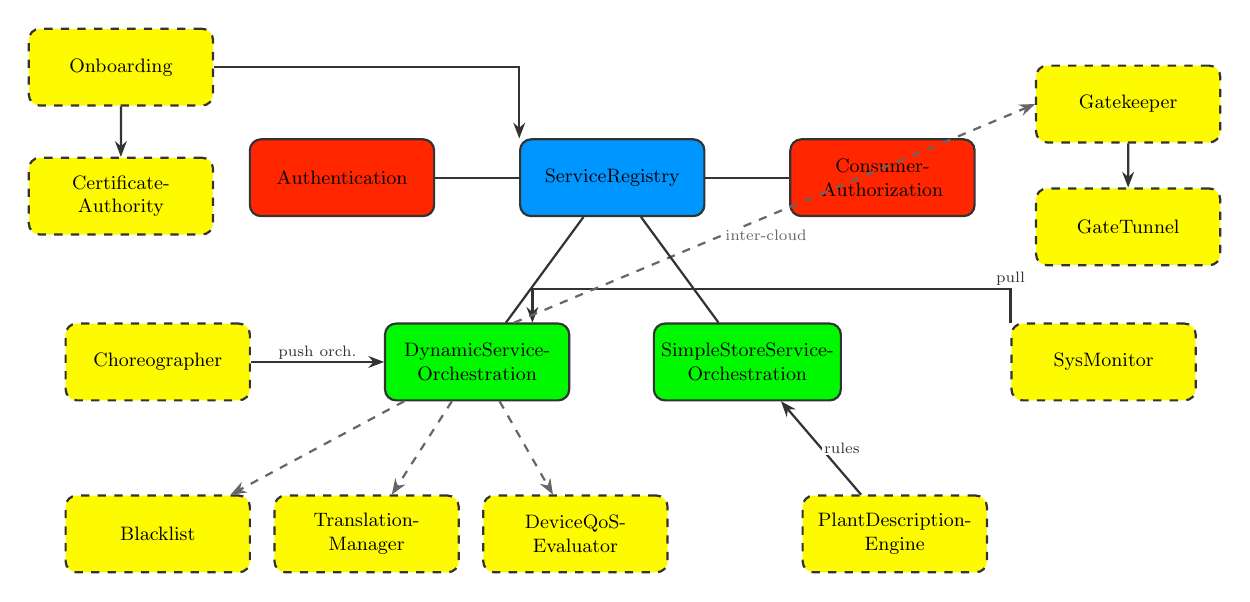
\begin{tikzpicture}[scale=0.78, every node/.style={transform shape}]
  \node[sr, ahRegistry]    (sr) at (0,0)    {ServiceRegistry};
  \node[authn, ahAuthentication] (an) at (-4.4,0) {Authentication};
  \node[authz, ahAuthorization] (az) at (4.4,0)  {Consumer-\\Authorization};
  \node[orch, ahOrchestration]  (do) at (-2.2,-3.0) {DynamicService-\\Orchestration};
  \node[orch, ahOrchestration]  (so) at (2.2,-3.0)  {SimpleStoreService-\\Orchestration};
  \node[sup] (bl) at (-7.4,-5.8) {Blacklist};
  \node[sup, ahSupport] (tm) at (-4.0,-5.8) {Translation-\\Manager};
  \node[sup, ahSupport] (qe) at (-0.6,-5.8) {DeviceQoS-\\Evaluator};
  \node[sup, ahSupport] (pde) at (4.6,-5.8) {PlantDescription-\\Engine};
  \node[sup, ahSupport] (ch) at (-7.4,-3.0) {Choreographer};
  \node[sup, ahSupport] (sm) at (8.0,-3.0) {SysMonitor};
  \node[sup, ahSupport] (ob) at (-8.0,1.8) {Onboarding};
  \node[sup, ahSupport] (ca) at (-8.0,-0.3) {Certificate-\\Authority};
  \node[sup, ahSupport] (gk) at (8.4,1.2) {Gatekeeper};
  \node[sup, ahSupport] (gt) at (8.4,-0.8) {GateTunnel};
  \draw[owire, -{Stealth[length=2mm]}] (do) -- (bl);
  \draw[owire, -{Stealth[length=2mm]}] (do) -- (tm);
  \draw[owire, -{Stealth[length=2mm]}] (do) -- (qe);
  \draw[wire, -{Stealth[length=2mm]}] (pde) -- node[lbl, right, font=\scriptsize]{rules} (so);
  \draw[wire, -{Stealth[length=2mm]}] (ch) -- node[lbl, above, font=\scriptsize]{push orch.} (do);
  \draw[wire, -{Stealth[length=2mm]}] (sm.north west) -- ($(sm.north west)+(0,0.55)$) node[lbl, above, font=\scriptsize, pos=1]{pull} -| ($(do.north)+(0.9,0)$);
  \draw[wire, -{Stealth[length=2mm]}] (ob) -- (ca);
  \draw[wire, -{Stealth[length=2mm]}] (ob.east) -- (sr.west |- ob.east) -- (sr.north west);
  \draw[wire, -{Stealth[length=2mm]}] (gk) -- (gt);
  \draw[owire, -{Stealth[length=2mm]}] ($(do.north)+(0.6,0)$) -- node[lbl, right, font=\scriptsize, pos=0.4]{inter-cloud} (gk.west);
  \foreach \n in {an,az,do,so} \draw[wire] (\n) -- (sr);
\end{tikzpicture}
\caption{Support systems around the Core (selection). Dashed arrows: consumed by advanced
orchestration when the feature is enabled; solid arrows: Support systems driving Core systems or
each other. All Support systems also register in the ServiceRegistry and use the authentication
and authorisation services; EventHandler, DataManager, TimeManager, Configuration and AIGym are
consumed by application systems and omitted.}
\label{fig:supcomp}
\end{figure}

\subsection{Common Properties of Support Systems}
\label{sec:sup:common}
All 5.2 Support systems share the following properties, which follow from the Core
architecture:
\begin{itemize}
  \item \textbf{Registration and discovery.} Each system registers itself and its services in the
        \sys{ServiceRegistry} and revokes them on shutdown. Systems that must search the whole
        registry (\sys{TranslationManager}, \sys{DeviceQoSEvaluator}, \sys{Choreographer},
        \sys{PlantDescriptionEngine}, \sys{SysMonitor}) are granted direct discovery access.
  \item \textbf{Identity.} Each system is identified by its Arrowhead certificate, optionally
        combined with an identity token from the \sys{Authentication} system.
  \item \textbf{Authorisation of produced services.} Application services are protected by
        certificate-based interface policies and, per call, by
        \sys{ConsumerAuthorization}~\svc{authorization}; ownership rules apply where the caller's
        identity is decisive (a system's own configuration, a session's owner, a step's
        executor, a bridge's translator).
  \item \textbf{Management.} Management services are protected by the management policy of the
        system, as for the Core systems, and every system provides \svc{generalManagement}.
  \item \textbf{Own data.} Each system owns its data store; no store is shared.
  \item \textbf{Observability.} Each system publishes periodic liveness, power and status
        observations through the \svc{sysMonitor} contract (Section~\ref{sec:sup:monitoring});
        its liveness reflects its own health, for example ``degraded'' while its store is
        unavailable or its time is untrusted.
\end{itemize}

\subsection{Orchestration Support}
\label{sec:sup:orch}

\subsubsection{Blacklist}
The \sys{Blacklist} system lets operators and authorised systems exclude named systems from the
local cloud for a period of time, with a mandatory reason. A system is excluded while at least one
unexpired entry exists for it. Every system that enables blacklist filtering checks each requester
with \svc{blacklistDiscovery} and rejects excluded ones; the advanced Orchestration system removes
excluded providers from its results. A blacklisted system can still look up why it is excluded.
Entries are created, removed and queried through \svc{blacklistManagement}; a configured whitelist
of systems, such as the \sys{Blacklist} itself, can never be excluded. Filtering can be configured
to fail closed when the \sys{Blacklist} system is unavailable.

\subsubsection{TranslationManager}
When no provider offers a service in a form the consumer can use -- a different protocol or a
different data model -- the advanced Orchestration system can ask the \sys{TranslationManager} to
create a \emph{translation bridge}. The \sys{TranslationManager} discovers \emph{interface
translators} that can reach the candidate providers and, if the data models differ, \emph{data
model translators}; it negotiates a bridge, obtains the tokens the translator needs, and returns
the bridge interface, which the consumer then uses like a normal service interface. Bridges have a
life cycle (discovered, initialised, used, closed, aborted, error); translators report usage and
termination through \svc{translationReport}. Management of bridges is offered through
\svc{translationBridgeManagement}.

\subsubsection{DeviceQoSEvaluator}
The \sys{DeviceQoSEvaluator} maintains quality data for the \emph{devices} hosting the systems of
the local cloud: network round-trip time and, where a device agent is installed, CPU load, memory
use and network load. It maps systems to devices from the registry content. Through
\svc{qualityEvaluation} the advanced Orchestration system asks it to \emph{filter} providers whose
device quality does not meet a threshold, or to \emph{sort} providers by device quality.
Measurements and the device map are administered through \svc{deviceQualityDataManagement}.

\subsection{Engineering and Automation}
\label{sec:sup:eng}

\subsubsection{PlantDescriptionEngine}
A \emph{plant description} is an engineered model of the local cloud: its systems, the services
each system consumes or produces (\emph{ports}), and the \emph{connections} between consumer and
producer ports, with priorities. The \sys{PlantDescriptionEngine} keeps one plant description
active and continuously reconciles the local cloud with it: it matches plant systems to registered
systems (by name and metadata), atomically replaces the corresponding managed snapshot in DynamicServiceOrchestration,
retaining empty scopes for unavailable producers and withdrawing scopes no longer described. Deviations -- a described
system that is not registered or is matched ambiguously, a registered system that is not
described, a system that is not monitored or has no recent observations -- are raised as
\emph{alarms} that operators acknowledge. Descriptions are managed through
\svc{plantDescriptionManagement}; descriptions and alarms are read through
\svc{plantDescriptionMonitor}. In the hierarchy of orchestration rule owners
(Section~\ref{sec:orch}), the \sys{PlantDescriptionEngine} realises the PlantDescription level.
Together with its engineering user interface it forms the management layer of the local cloud
(Section~\ref{sec:mgmt}); it is operational in the 5.2.2 test beds.

\subsubsection{Choreographer}
The \sys{Choreographer} executes pre-defined workflows (\emph{plans}). A plan is a chain of
\emph{actions}; an action is a graph of \emph{steps}, where each step states a service requirement
and parameters, and independent steps run in parallel. \emph{Executors} are application systems
that register with the \sys{Choreographer} and perform steps. For each step the \sys{Choreographer}
selects an executor and has the advanced Orchestration system orchestrate the required provider
\emph{for the executor} by push orchestration, so that authorisation and tokens apply to the
executor; it then starts the executor, which reports completion. A failed executor is excluded
and the step retried with another one. Clients start and abort sessions through
\svc{choreographerSession}; executors use \svc{choreographerExecutor}; plans, sessions, executors
and the work log are managed through \svc{choreographerManagement}.

\subsubsection{Configuration}
The \sys{Configuration} system stores one configuration file per system and lets each system fetch
its own file at run time (\svc{configuration}); a system can only read its own configuration.
Authorised systems can read and store configurations on behalf of others
(\svc{configurationProxy}), and operators manage all configurations
(\svc{configurationManagement}). Together with lookup, this lets systems keep only the
\sys{ServiceRegistry} address and their credentials as local configuration.

\subsection{Security and Life Cycle}
\label{sec:sup:sec}

\subsubsection{CertificateAuthority}
The \sys{CertificateAuthority} issues the X.509 certificates by which systems are identified. It
signs certificate requests submitted by authorised provisioning systems (the \sys{Onboarding}
system or an operator), never issues certificates with signing capability, and records every issued
certificate. Through \svc{certificateValidation} any system of the local cloud can check whether a
certificate was issued by the local cloud and is valid and not revoked, and whether a trusted public
key is valid. Revocation and trusted keys are managed through \svc{certificateAuthorityManagement}.

\subsubsection{Onboarding}
As the Arrowhead architecture relies on storing metadata about systems for orchestration,
choreography and so on, every system in every local cloud must be referable unambiguously; that
reference is its \emph{identity}. \emph{Onboarding} is the process by which a new device and the
systems it hosts obtain identities and the information they need to join the local cloud;
\emph{off-boarding} is its reverse. The \sys{Onboarding} system implements the complete procedure
after Bicaku et al.\ \cite{bicaku2018}: an operator approves a device by the fingerprint of its
manufacturer-issued bootstrap certificate and names the systems it may host
(\svc{onboardingManagement}); the device then obtains, step by step through the \svc{onboarding}
service, an onboarding certificate, a device certificate and registry entry, and per approved
system a system certificate and an identity, each step requiring the credential of the previous
one. Off-boarding withdraws all of it. Every certificate is signed by the
\sys{CertificateAuthority}; enrolment is by certificate only. Onboarding is the admission-control
mechanism of the framework (Section~\ref{sec:secmech}); the procedure is shown in
Section~\ref{sec:uc:onboarding}.

\subsection{Information and Messaging}
\label{sec:sup:info}

\subsubsection{EventHandler}
The \sys{EventHandler} decouples producers and consumers of \emph{events}. Systems subscribe
(\svc{eventSubscription}) to an event type, optionally with a metadata filter and a
validity window, and give a notification address. Publishers publish events (\svc{eventPublish});
the \sys{EventHandler} delivers each event to all matching subscribers. Publisher and subscriber
identities are taken from authentication, never from the message. Subscriptions are administered
through \svc{eventHandlerManagement}.

\subsubsection{DataManager}
The \sys{DataManager} handles measurement and actuation data in the SenML format. Its
\svc{dataProxy} service keeps the latest values per system and service, so that consumers can read
data without contacting the producer; its \svc{dataHistorian} service stores data over time and
answers time-window queries per signal.

\subsubsection{TimeManager}
The \sys{TimeManager} provides the current time, the time zone of the local cloud and an assessment
of whether the time can be \emph{trusted} (\svc{time}). It compares its clock with external time
servers and reports the time as trusted only while the deviation is below a threshold; it is
untrusted until the first successful comparison.

\subsection{Monitoring and Analytics}
\label{sec:sup:monitoring}

\subsubsection{The sysMonitor Contract}
Operating a local cloud requires knowing whether its microsystems are alive and healthy. As a
project proposal for 5.2, every microsystem -- Core, Support and application -- provides a
\svc{sysMonitor} service: it periodically publishes \emph{observations}, at least \op{echo}
(alive or degraded), \op{power} and \op{status}, each carrying the provider, observation type,
source time, sequence number, value, unit and quality. Observations are published over AMQP with
mutual TLS to a topic exchange of the local cloud's AMQP broker, under the publishing system's own
certificate, as persistent messages confirmed by the broker; the routing key names the cloud, the
system, the service instance and the observation type \cite{sysmonamqp}. The broker lets each
system publish only under its own routing keys and bind its queues only to the keys it is entitled
to. The service is registered like any other, with an AMQP interface template, and access to each
system's observations is governed by the Authorisation system. The AMQP broker carries only
\svc{sysMonitor}; the local cloud's MQTT broker remains in place for all other MQTT traffic.
Liveness probes over HTTP, where still offered, are registered as a separate \svc{echo} service.

\subsubsection{SysMonitor}
The \sys{SysMonitor} system collects the observations of all monitored microsystems. It finds
the \svc{sysMonitor} providers through the advanced Orchestration system, so it follows only the
providers it is authorised for, receives their observations from the AMQP broker in a durable
queue bound to the selected providers and observation types, validates and de-duplicates them,
and stores them for a retention period. It provides the stored history (\svc{sysMonitorHistory}),
a normalised stream of observations over MQTT (\svc{sysMonitorData}) and operator management
(\svc{sysMonitorManagement}), with which operators select the providers and observation types to
receive. The
\sys{PlantDescriptionEngine} uses the history to detect systems that are not monitored or not alive.
(A former \sys{SysMonitorPublisher} published observations on behalf of systems without their own
publisher; it is deprecated now that all 5.2 systems publish themselves.)

\subsubsection{AIGym}
The \sys{AIGym} is a sandbox for experiments with models on local-cloud data. It subscribes to the
normalised monitoring stream (\svc{sysMonitorData}, MQTT) and lets authorised systems add labelled samples, obtain predictions
and read recent observations (\svc{aiGym}).

\subsection{Inter-Cloud}
\label{sec:sup:intercloud}

\subsubsection{Gatekeeper}
Each local cloud that takes part in a system of local clouds has a \sys{Gatekeeper}, its single
point of contact for other local clouds. Through \svc{globalServiceDiscovery} it searches
neighbouring local clouds for a service; through \svc{interCloudNegotiation} it negotiates with the
\sys{Gatekeeper} of a provider's cloud that a local consumer may use a remote provider. The
provider's \sys{Gatekeeper} answers only with providers that its own Authorisation system grants
to that consumer of that cloud. Neighbour clouds and relays are administered through
\svc{gatekeeperManagement}.

\subsubsection{GateTunnel}
When a consumer and a remote provider cannot reach each other directly, the \sys{GateTunnel}s of
the two local clouds carry the service exchange of a negotiated \emph{session}: the consumer's
\sys{GateTunnel} offers a local endpoint for that consumer only, forwards its requests to the
provider's \sys{GateTunnel}, which calls the provider and returns the response. Sessions are opened
by the \sys{Gatekeeper}s (\svc{gateTunnelConnection}); \svc{gateTunnelKey} provides the public key
for securing a session, and \svc{gateTunnelManagement} lets operators supervise sessions. It
succeeds the 4.x Gateway.

\subsubsection{The Inter-Cloud Relay}
\label{sec:sup:relay}
\sys{Gatekeeper}s and \sys{GateTunnel}s of different local clouds communicate through an
\emph{inter-cloud relay} \cite{relay}: a message broker of the organisation (MQTT with mutual TLS) that every
participating local cloud can reach. The relay carries global service discovery and inter-cloud
negotiation messages between \sys{Gatekeeper}s, and the requests and responses of sessions between
\sys{GateTunnel}s. Trust between the clouds is established by an \emph{organisation certificate
authority} that cross-certifies each local cloud's CA; each cross-certificate is
\emph{name-constrained} to its own cloud, so a cloud CA can vouch towards the relay only for
identities of its own cloud. \sys{Gatekeeper}s and \sys{GateTunnel}s use dedicated relay identities
for this purpose, not their ordinary cloud certificates; inside a local cloud only the cloud's own
CA is trusted. The relay's access rules let each \sys{Gatekeeper} and \sys{GateTunnel} read only its
own cloud's inbox for its own role and write into another cloud's inbox only under its own
identity, so a receiver takes the sender's identity and cloud from the authenticated channel, never
from the message body.

\subsection{Deploying Support Systems in a Local Cloud}
\label{sec:sup:deploy}
Support systems are started after the Core systems (Section~\ref{sec:bootstrap}, step 5). Beyond
the general prerequisites -- an identity, registration rights and access rules -- some Support
systems require explicit Core configuration:
\begin{itemize}
  \item Direct discovery access in the \sys{ServiceRegistry} for systems that search the whole
        registry (Section~\ref{sec:sup:common}).
  \item Management rights: the \sys{PlantDescriptionEngine} manages registry queries and
        orchestration rules; the \sys{Choreographer} manages push orchestration; the advanced
        Orchestration system and the \sys{TranslationManager} generate tokens on behalf of
        consumers.
  \item Access rules for every consumer of a Support service and for the \sys{SysMonitor} on every
        \svc{sysMonitor} provider.
  \item The orchestration approach: PDE, workflows and monitoring now use DSO in the local Java
        profile. PDE requires the managed-rule extension and schema upgrade. SimpleStore may
        still run independently for clients that explicitly select the atomic approach.
  \item For onboarding: the \sys{Onboarding} system needs the rights to have certificates signed
        and revoked, to create and remove identities, to manage registry entries and to exclude
        systems; approving devices requires an operator.
\end{itemize}
Canonical ports of all Support systems are allocated by the port numbering of
Section~\ref{sec:nfr:ports}.


\subsection{The System-Service Matrix}
\label{sec:matrix}

To keep track of what services are produced and consumed by different systems, we use a
system-service matrix. It outlines the Core and Support systems in terms of the services they
provide and consume, and refers both to the abstract definitions of the services (SDs) and to
the available implementations of the systems, whose interfacing details are documented in IDDs.
The matrix is given in Appendix~\ref{app:matrix}.



\newpage
%% ============================================================================================

\FloatBarrier





\section{Management Layer and Security Mechanisms}
\label{sec:mgmtsec}

Two capabilities of the 5.2 framework span several Core and Support systems and are therefore
described here as wholes: the \emph{management layer}, through which engineers and operators state
how the local cloud shall be composed, and the set of \emph{security mechanisms}, to which the
\sys{Onboarding} system adds controlled admission and withdrawal of devices and systems.

\subsection{The Management Layer}
\label{sec:mgmt}

The Core systems form the control plane of a local cloud (Section~\ref{sec:planes}): they decide,
request by request, who may talk to whom and how. What the local cloud \emph{should} look like --
which systems belong to the plant and which consumer shall use which producer -- is engineering
knowledge that lies above the control plane. Release 5.2 makes this a separate, operational
\emph{management layer} (Figure~\ref{fig:layers}):

\begin{figure}[h!]
\centering
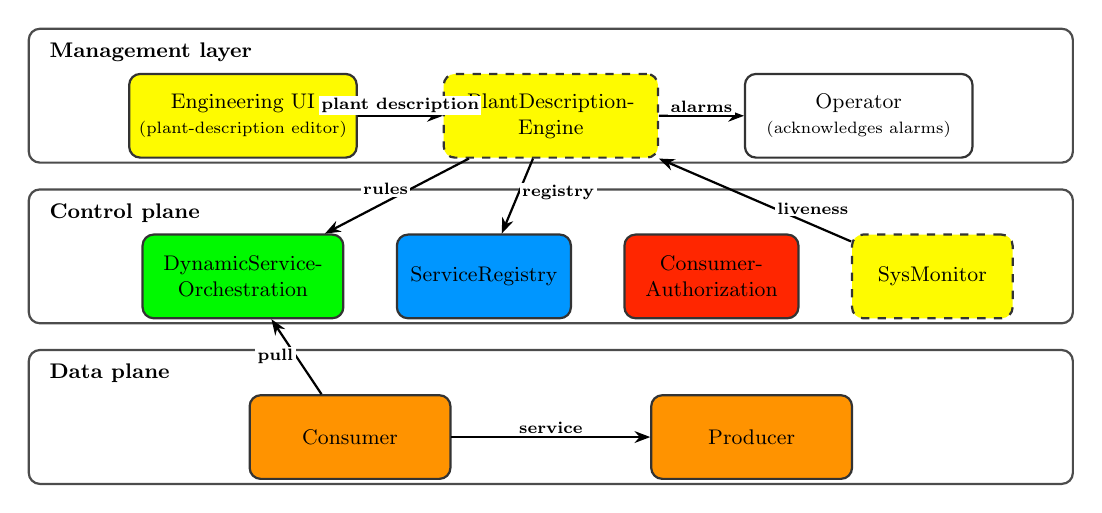
\begin{tikzpicture}[scale=0.85, every node/.style={transform shape}]
  \tikzset{band/.style={draw=black!70, thick, rounded corners=4pt, minimum width=15.6cm, minimum height=2.0cm},
           blbl/.style={font=\small\bfseries, anchor=west, align=left}}
  \node[band, fill=white]  (ml) at (0,4.6) {};
  \node[band, fill=white] (cp) at (0,2.2) {};
  \node[band, fill=white] (dp) at (0,-0.2) {};
  \node[blbl] at ($(ml.west)+(0.2,0.65)$) {Management layer};
  \node[blbl] at ($(cp.west)+(0.2,0.65)$) {Control plane};
  \node[blbl] at ($(dp.west)+(0.2,0.65)$) {Data plane};
  \node[comp, fill=white, minimum width=3.4cm, ahSupport] (ui) at (-4.6,4.3) {Engineering UI\\{\scriptsize (plant-description editor)}};
  \node[sup, minimum width=3.2cm, ahSupport] (pde) at (0,4.3) {PlantDescription-\\Engine};
  \node[comp, fill=white, minimum width=3.4cm] (op) at (4.6,4.3) {Operator\\{\scriptsize (acknowledges alarms)}};
  \node[orch, minimum width=3.0cm, ahOrchestration] (so) at (-4.6,1.9) {DynamicService-\\Orchestration};
  \node[sr, minimum width=2.6cm, ahRegistry]   (sr) at (-1.0,1.9) {ServiceRegistry};
  \node[authz, minimum width=2.6cm, ahAuthorization] (az) at (2.4,1.9) {Consumer-\\Authorization};
  \node[sup, minimum width=2.4cm, ahSupport]   (sm) at (5.7,1.9) {SysMonitor};
  \node[app] (co) at (-3.0,-0.5) {Consumer};
  \node[app] (pr) at (3.0,-0.5) {Producer};
  \draw[msg] (ui) -- node[lbl, above]{plant description} (pde);
  \draw[msg] (pde) -- node[lbl, left, pos=0.4]{rules} (so);
  \draw[msg] (pde) -- node[lbl, right, pos=0.45]{registry} (sr);
  \draw[msg] (sm) -- node[lbl, right, pos=0.4]{liveness} (pde.south east);
  \draw[msg] (pde) -- node[lbl, above]{alarms} (op);
  \draw[msg] (co) -- node[lbl, left]{pull} (so);
  \draw[msg] (co) -- node[lbl, above]{service} (pr);
\end{tikzpicture}
\caption{The management layer above the control and data planes. Engineering intent enters as a
plant description, becomes orchestration rules, and is checked against the running cloud.}
\label{fig:layers}
\end{figure}

\begin{description}
  \item[Engineering intent.] An engineer describes the plant -- its systems, the services each
        consumes or produces (ports) and the connections between them, with priorities -- as a
        \emph{plant description}. Plant descriptions can include each other, so that a plant can be
        composed of line or cell descriptions. One description is active at a time.
  \item[Enforcement.] The \sys{PlantDescriptionEngine} turns the active description into
        orchestration rules of DynamicServiceOrchestration and keeps them in step with the
        registry: a connection becomes rules as soon as both its systems are registered and
        identifiable, and its rules are withdrawn when it is removed from the description. In the
        hierarchy of rule owners (Section~\ref{sec:orch}) these rules are the
        \emph{PlantDescription} level: engineered, therefore above the orchestration system's own
        decisions and the consumer's preferences, and below explicit operator decisions.
  \item[Supervision.] The \sys{PlantDescriptionEngine} compares the running local cloud with the
        description and raises \emph{alarms}: a described system that is missing or ambiguous, a
        running system that is not described, a system that is not monitored or has gone silent
        (from the \sys{SysMonitor} history). Operators acknowledge alarms.
  \item[Engineering UI.] The first engineering user interface of the framework is the
        plant-description editor of the local-cloud operator console. It lists the stored plant
        descriptions and edits them in a form -- systems and their ports, connections with
        priorities, includes, activation -- or directly as the plant-description document, and
        stores them through \svc{plantDescriptionManagement}; alarms are read through
        \svc{plantDescriptionMonitor}, which the first UI does not yet display. A companion view shows, for each
        provider and service, which consumers are \emph{authorised} and which are
        \emph{orchestrated} to it, so that engineered intent and access rules can be compared.
\end{description}

The management layer has no privileged path into the local cloud. The engineering UI acts through
the \sys{PlantDescriptionEngine}'s management service, and the \sys{PlantDescriptionEngine} acts
through the management services of the \sys{ServiceRegistry} and DynamicServiceOrchestration;
each of these is protected by the management policy of the providing system
(Section~\ref{sec:sysdesc}), and the console is a client that must be granted management rights
like any other. The updated Java management layer uses DSO alone; the earlier test-bed setup required SSO
next to DSO. Deployment requires the DSO managed-rule extension and schema migration.

\subsection{Security Mechanisms of the Arrowhead Framework}
\label{sec:secmech}

Full AAA security and encryption of exchanged information are the default from
v5.0. They are realised by cooperating mechanisms at different points in a system's
life (Table~\ref{tab:secmech}); they are not optional additions to discovery.
The 5.2.2 description additionally covers explicit admission and withdrawal through
\sys{Onboarding}, which complements the existing security baseline.

\begin{table}[h!]
\centering\footnotesize
\begin{tabularx}{\textwidth}{|P{3.6cm}|Y|P{4.0cm}|}\hline
\rowcolor{gray!33}Mechanism & What it decides & Provided by \\\hline
Admission and withdrawal (onboarding, off-boarding) & Which devices and systems may obtain credentials at all, and when they lose them & \sys{Onboarding}, \sys{CertificateAuthority} \\\hline
Encrypted communication & Confidentiality and integrity of exchanged information, including bootstrap, management and application traffic & Authenticated TLS endpoints and brokers; end-to-end protection for the selected federation profile \\\hline
Certificate-based identity & Who is communicating (mutual TLS, local-cloud certificates) & \sys{CertificateAuthority}; every system \\\hline
Identity tokens & Who is communicating, as a short-lived token bound to the certificate & \sys{Authentication} \\\hline
Authorisation rules & Who may consume which service and operation; management rules take priority & \sys{ConsumerAuthorization} \\\hline
Access tokens & A short-lived credential per consumer, provider and service & \sys{ConsumerAuthorization} \\\hline
Restricted discovery & Which service metadata can be found directly; direct discovery does not waive authentication or provider authorisation & \sys{ServiceRegistry} \\\hline
Management policy & Who may administer a system & every system \\\hline
Exclusion & Which systems are barred from the local cloud for a period & \sys{Blacklist} \\\hline
Inter-cloud trust & Which other local clouds' \sys{Gatekeeper}s and \sys{GateTunnel}s are accepted & Organisation CA (name-constrained cross-certificates), relay access rules, provider-side authorisation \\\hline
\end{tabularx}
\caption{Security mechanisms of the Arrowhead Framework 5.2.2.}
\label{tab:secmech}
\end{table}

\paragraph{Onboarding as admission control.} Without onboarding, credentials are provisioned out of
band, and the local cloud cannot tell which device a system runs on or whether its credential was
ever meant to be issued. The \sys{Onboarding} system makes admission an explicit, operator-controlled
procedure and builds a chain of trust from the hardware device to its hosted systems:
\begin{enumerate}
  \item An operator \emph{approves} a device: its manufacturer-issued bootstrap certificate
        (identified by fingerprint) and the systems it may host. Nothing else can enrol.
  \item With the approved bootstrap certificate the device obtains a short-lived
        \emph{onboarding certificate}; with that, a \emph{device certificate} and its registry entry;
        with that, per approved system, a \emph{system certificate} and an identity. Each credential
        can be obtained only with the previous one, and only the latest valid credential of each
        kind is accepted.
  \item The systems then authenticate, register and are authorised like any other system: admission
        does not grant rights; access rules remain the operator's decision.
  \item \emph{Off-boarding}, by the device or the operator, withdraws everything the procedure
        created: registry entries and identities are removed, certificates revoked, and the systems
        excluded.
\end{enumerate}
All certificates are signed by the \sys{CertificateAuthority}; the \sys{Onboarding} system holds no
signing key. Onboarding thus complements the mechanisms that follow it: authentication and
authorisation decide what a credential may do, onboarding decides whether the credential exists. Its
withdrawal is fully effective only where the other mechanisms honour it -- where revocation is
checked and exclusion is enforced (Section~\ref{sec:issues}).

\newpage
%% ============================================================================================


\section{Use-cases}
\label{sec:usecases}

\paragraph{Security precondition for every use case.}
All exchanges below assume the v5.0 default: authenticated participants, positive
authorisation and encrypted information exchange. Each diagram isolates one
function; omitted TLS handshakes or policy calls are not permission to disable them.


To make it more apparent how the Arrowhead Core and Support systems can be used in practical
scenarios, we present twelve use cases: five on the Core systems
(Sections~\ref{sec:uc:discovery}--\ref{sec:uc:both}) and seven involving Support systems
(Sections~\ref{sec:uc:onboarding}--\ref{sec:uc:intercloud}). Each centres around a sequence diagram illustrating how systems consume
each other's services. Messages are labelled with the service definition and operation that
realise them in 5.2.2.

\subsection{Service Discovery}
\label{sec:uc:discovery}

The first and most basic use case shows how system B can consume service \svc{a}, provided by
A, by looking up its address in ServiceRegistry. The default AAA and encryption
baseline remains active; this diagram isolates lookup and omits the security
exchanges. B has an explicit right to discover this service directly, A and B know
the trusted registry's address, and A enforces B's permission before executing
\svc{a}. An open discovery setting does not disable authentication or provider
access control.

\begin{figure}[h!]
\centering
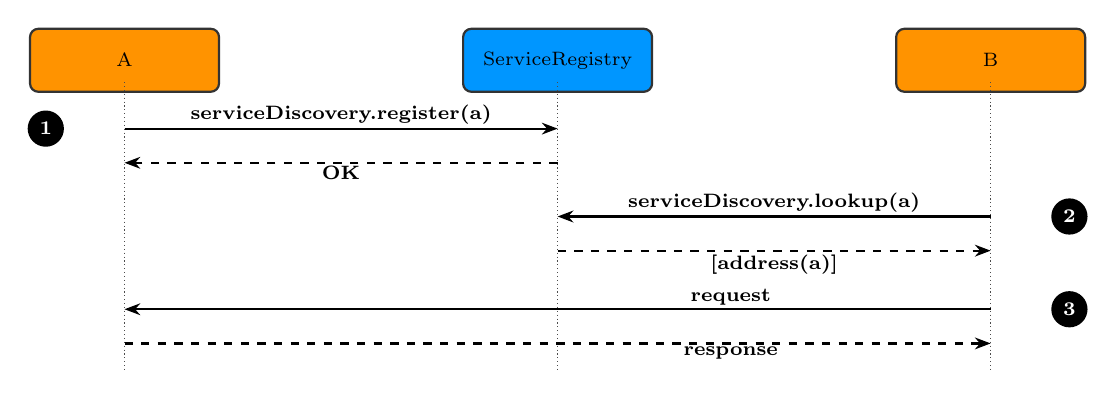
\begin{tikzpicture}[yscale=0.62]
  \seqhead{6.4}{0}{A}{fill=AppOrange, ahApplication}
  \seqhead{6.4}{5.5}{ServiceRegistry}{fill=SRBlue, ahRegistry}
  \seqhead{6.4}{11}{B}{fill=AppOrange, ahApplication}
  \node[num] at (-1.0,-1.4) {1};
  \draw[msg] (0,-1.4) -- node[lbl, above]{serviceDiscovery.register(a)} (5.5,-1.4);
  \draw[ret] (5.5,-2.1) -- node[lbl, below]{OK} (0,-2.1);
  \node[num] at (12.0,-3.2) {2};
  \draw[msg] (11,-3.2) -- node[lbl, above]{serviceDiscovery.lookup(a)} (5.5,-3.2);
  \draw[ret] (5.5,-3.9) -- node[lbl, below]{[address(a)]} (11,-3.9);
  \node[num] at (12.0,-5.1) {3};
  \draw[msg] (11,-5.1) -- node[lbl, above, pos=0.3]{request} (0,-5.1);
  \draw[ret] (0,-5.8) -- node[lbl, below, pos=0.7]{response} (11,-5.8);
\end{tikzpicture}
\caption{Service discovery.}
\label{fig:uc1}
\end{figure}

The use case consists of three message exchanges:
\begin{enumerate}
  \item A registers its service \svc{a} with the \sys{ServiceRegistry}, which accepts the
        registration.
  \item Later, B looks up \svc{a} via the \sys{ServiceRegistry}, which responds with the network
        address and other details of \svc{a}.
  \item B consumes \svc{a} by sending a request to A, which responds with some status and
        payload of relevance to the service.
\end{enumerate}
As only one instance of \svc{a} was registered, the response in exchange 2 contained only one
address. If more instances had been registered, B would have received all of them and would have
had to determine itself which instance is most appropriate, perhaps by looking at metadata in
the registrations. Alternatively, B could have looked up a particular service instance
identifier instead of a service definition; since identifiers are unique, the result contains at
most one entry. This requires the identifier to be known in advance and the instance to be online
when B needs it. Another approach is to centralise decisions about service consumption in an
Orchestration system (Section~\ref{sec:uc:orch}). In a local cloud with restricted discovery,
this use case is only available to systems granted direct access.

\subsection{Authenticated Access}
\label{sec:uc:authn}

The second use case shows the identity-token part of AAA over an already encrypted,
mutually authenticated channel. A and B have trusted local-cloud certificates and
pre-registered identities in \sys{Authentication}. TLS setup is omitted from the
sequence diagram, not from the security requirements. Authorisation is shown
separately in the following use case and remains required before service execution.

\begin{figure}[h!]
\centering
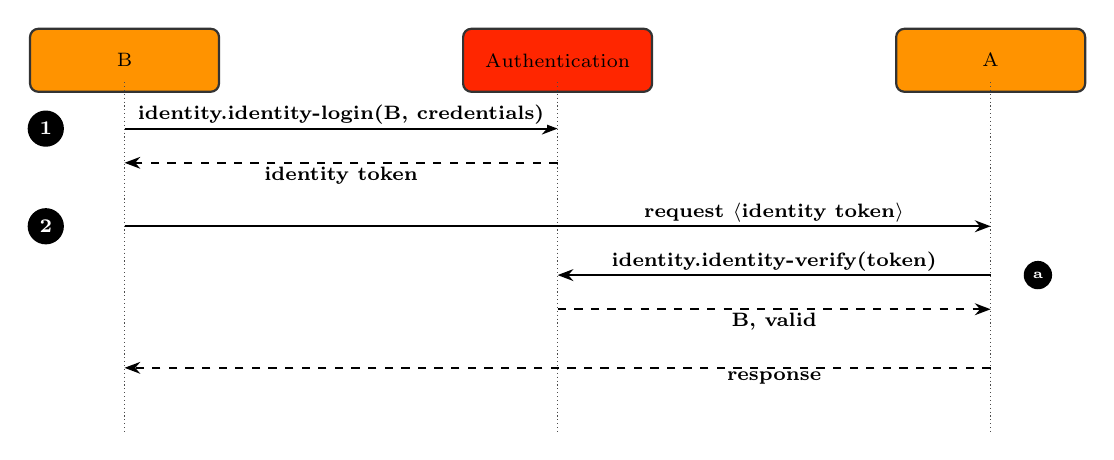
\begin{tikzpicture}[yscale=0.62]
  \seqhead{7.6}{0}{B}{fill=AppOrange, ahApplication}
  \seqhead{7.6}{5.5}{Authentication}{fill=AuthnLilac, ahAuthentication}
  \seqhead{7.6}{11}{A}{fill=AppOrange, ahApplication}
  \node[num] at (-1.0,-1.4) {1};
  \draw[msg] (0,-1.4) -- node[lbl, above]{identity.identity-login(B, credentials)} (5.5,-1.4);
  \draw[ret] (5.5,-2.1) -- node[lbl, below]{identity token} (0,-2.1);
  \node[num] at (-1.0,-3.4) {2};
  \draw[msg] (0,-3.4) -- node[lbl, above, pos=0.75]{request $\langle$identity token$\rangle$} (11,-3.4);
  \node[sub] at (11.6,-4.4) {a};
  \draw[msg] (11,-4.4) -- node[lbl, above]{identity.identity-verify(token)} (5.5,-4.4);
  \draw[ret] (5.5,-5.1) -- node[lbl, below]{B, valid} (11,-5.1);
  \draw[ret] (11,-6.3) -- node[lbl, below, pos=0.25]{response} (0,-6.3);
\end{tikzpicture}
\caption{Authenticated access with an identity token.}
\label{fig:uc2}
\end{figure}

\begin{enumerate}
  \item B logs in to the \sys{Authentication} system with its credentials and receives a
        time-limited identity token. (The address of the \svc{identity} service is obtained from
        the \sys{ServiceRegistry}, where it is always directly discoverable.)
  \item B sends its request to A and includes the identity token.
        \begin{enumerate}[label=(\alph*)]
          \item A asks the \sys{Authentication} system to verify the token and learns that the
                requester is B; only then does A process the request.
        \end{enumerate}
\end{enumerate}
In the default reference token profile, A also requires the verified token identity
to match B's authenticated certificate. A certificate-only binding derives identity
from mutual TLS instead of exchanges 1 and 2a; it still requires authorisation and
encryption. Neither mechanism makes a self-declared identity sufficient.

\subsection{Authorisation}
\label{sec:uc:authz}

In this use case we add access control through the Authorisation system. Whenever an attempt is
made to consume a service, the providing system validates the request by consulting
\sys{ConsumerAuthorization} before responding. We assume that all services were registered in
the \sys{ServiceRegistry} before the use case begins, that the requesters are authenticated as
in Section~\ref{sec:uc:authn}, and that \sys{ConsumerAuthorization} has been provided with an
appropriate set of access rules.

\begin{figure}[h!]
\centering
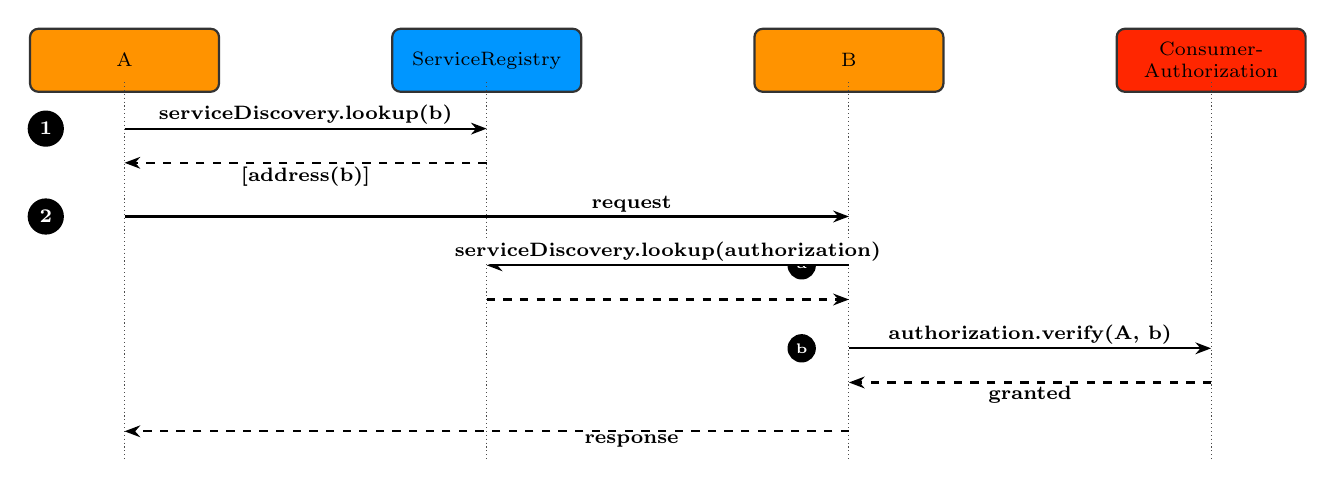
\begin{tikzpicture}[yscale=0.62]
  \seqhead{8.2}{0}{A}{fill=AppOrange, ahApplication}
  \seqhead{8.2}{4.6}{ServiceRegistry}{fill=SRBlue, ahRegistry}
  \seqhead{8.2}{9.2}{B}{fill=AppOrange, ahApplication}
  \seqhead{8.2}{13.8}{Consumer-\\Authorization}{fill=AuthzRed, ahAuthorization}
  \node[num] at (-1.0,-1.4) {1};
  \draw[msg] (0,-1.4) -- node[lbl, above]{serviceDiscovery.lookup(b)} (4.6,-1.4);
  \draw[ret] (4.6,-2.1) -- node[lbl, below]{[address(b)]} (0,-2.1);
  \node[num] at (-1.0,-3.2) {2};
  \draw[msg] (0,-3.2) -- node[lbl, above, pos=0.7]{request} (9.2,-3.2);
  \node[sub] at (8.6,-4.2) {a};
  \draw[msg] (9.2,-4.2) -- node[lbl, above]{serviceDiscovery.lookup(authorization)} (4.6,-4.2);
  \draw[ret] (4.6,-4.9) -- (9.2,-4.9);
  \node[sub] at (8.6,-5.9) {b};
  \draw[msg] (9.2,-5.9) -- node[lbl, above]{authorization.verify(A, b)} (13.8,-5.9);
  \draw[ret] (13.8,-6.6) -- node[lbl, below]{granted} (9.2,-6.6);
  \draw[ret] (9.2,-7.6) -- node[lbl, below, pos=0.3]{response} (0,-7.6);
\end{tikzpicture}
\caption{Authorisation by the provider.}
\label{fig:uc3}
\end{figure}

\begin{enumerate}
  \item A looks up \svc{b} via the \sys{ServiceRegistry}, which responds with the network address
        of \svc{b}. This requires A to have direct discovery access; in a local cloud with
        restricted discovery A would use orchestration instead (Section~\ref{sec:uc:both}).
  \item A attempts to consume \svc{b} by sending a request to B, which later responds. Before
        responding, B must ascertain that A is permitted to consume \svc{b}:
        \begin{enumerate}[label=(\alph*)]
          \item Since B does not yet know the network address of \sys{ConsumerAuthorization}, it
                looks it up; the \svc{authorization} service is always directly discoverable.
          \item B asks \sys{ConsumerAuthorization} whether A is permitted to consume its instance
                of \svc{b}, which it is. Management-level rules are evaluated first and take
                priority over B's own provider-level rules.
        \end{enumerate}
\end{enumerate}
Using authorisation in this manner means that access rules must be prepared and provided to
\sys{ConsumerAuthorization} in advance. As rules contain the unique identifiers of the systems
and services of the local cloud, those identifiers must be known in advance, and every system must
be preconfigured with its own identity. The need for preconfiguring rules can be reduced by rules
based on system metadata, or by a separate system that creates access rules dynamically according
to given strategies (for example the \sys{PlantDescriptionEngine}).

Compared with the 5.0 description, the \sys{ServiceRegistry} no longer consults the
Authorisation system on each lookup; instead its discovery policy restricts what can be
discovered directly, and the Authorisation system is consulted for management operations and by
orchestration.

\subsection{Orchestration}
\label{sec:uc:orch}

As noted in Section~\ref{sec:uc:discovery}, using only a \sys{ServiceRegistry} means that we must
rely on either (1) systems being able to choose what specific service instances to consume, or
(2) preconfiguring each system with the identifiers of those instances. With an Orchestration
system, both can be avoided by having the systems ask what services they should consume. We
assume that all services were registered before the use case begins and, for atomic
orchestration, that the Orchestration system has been provided with appropriate orchestration
rules. Authentication, authorisation and encrypted transport remain active; their
exchanges are omitted here to isolate service selection.

\begin{figure}[h!]
\centering
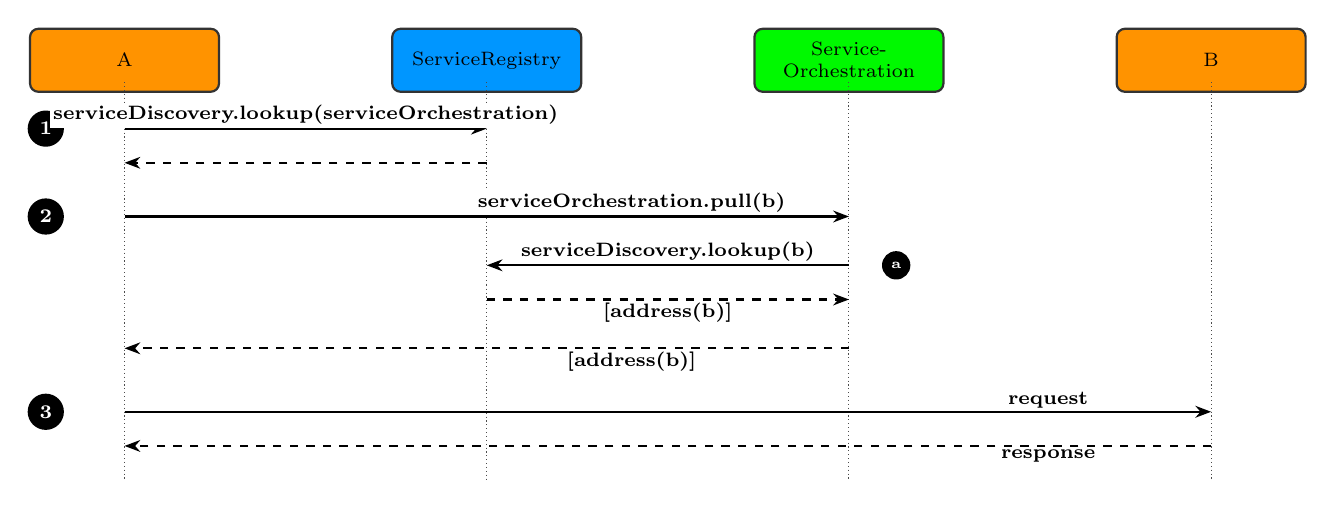
\begin{tikzpicture}[yscale=0.62]
  \seqhead{8.6}{0}{A}{fill=AppOrange, ahApplication}
  \seqhead{4.6}{4.6}{ServiceRegistry}{fill=SRBlue, ahRegistry}
  \seqhead{8.6}{9.2}{Service-\\Orchestration}{fill=OrchGreen, ahOrchestration}
  \seqhead{8.6}{13.8}{B}{fill=AppOrange, ahApplication}
  \draw[lifeline] (4.6,-4.6) -- (4.6,-8.6);
  \node[num] at (-1.0,-1.4) {1};
  \draw[msg] (0,-1.4) -- node[lbl, above]{serviceDiscovery.lookup(serviceOrchestration)} (4.6,-1.4);
  \draw[ret] (4.6,-2.1) -- (0,-2.1);
  \node[num] at (-1.0,-3.2) {2};
  \draw[msg] (0,-3.2) -- node[lbl, above, pos=0.7]{serviceOrchestration.pull(b)} (9.2,-3.2);
  \node[sub] at (9.8,-4.2) {a};
  \draw[msg] (9.2,-4.2) -- node[lbl, above]{serviceDiscovery.lookup(b)} (4.6,-4.2);
  \draw[ret] (4.6,-4.9) -- node[lbl, below]{[address(b)]} (9.2,-4.9);
  \draw[ret] (9.2,-5.9) -- node[lbl, below, pos=0.3]{[address(b)]} (0,-5.9);
  \node[num] at (-1.0,-7.2) {3};
  \draw[msg] (0,-7.2) -- node[lbl, above, pos=0.85]{request} (13.8,-7.2);
  \draw[ret] (13.8,-7.9) -- node[lbl, below, pos=0.15]{response} (0,-7.9);
\end{tikzpicture}
\caption{Orchestration (pull), advanced approach. With atomic orchestration, step 2a is
omitted, the response contains instance identifiers only, and A resolves them in the
\sys{ServiceRegistry}.}
\label{fig:uc4}
\end{figure}

\begin{enumerate}
  \item A looks up the network address of the \svc{serviceOrchestration} service through the
        \svc{serviceDiscovery} service of the \sys{ServiceRegistry}.
  \item A asks the Orchestration system which service instances it should consume, and the
        Orchestration system responds with the network address of \svc{b}, provided by B.
        \begin{enumerate}[label=(\alph*)]
          \item Since the advanced Orchestration system holds no network addresses itself, it
                consults the \sys{ServiceRegistry}, to which it has direct access.
        \end{enumerate}
  \item A consumes \svc{b} of B by sending a request, which B responds to.
\end{enumerate}
In this use case the orchestration information was \emph{pulled} by A. The Orchestration system
also supports \emph{push}: A subscribes to orchestration for \svc{b} and receives results whenever
the subscription is triggered, for example when its rules change. Pushing means that changes
reach their systems more reliably and more quickly than periodic pulls.

\subsection{Authorisation and Orchestration}
\label{sec:uc:both}

There is one important reason to consider authorisation and orchestration together: the advanced
Orchestration system can filter providers by the consumer's access rights and distribute access
tokens, which increase security because the credentials actually passed between systems expire
quickly. We assume that all services were registered before the use case begins, that A has
already looked up the address of the Orchestration system, and that \sys{ConsumerAuthorization}
has been provided with an appropriate set of access rules.

\begin{figure}[h!]
\centering
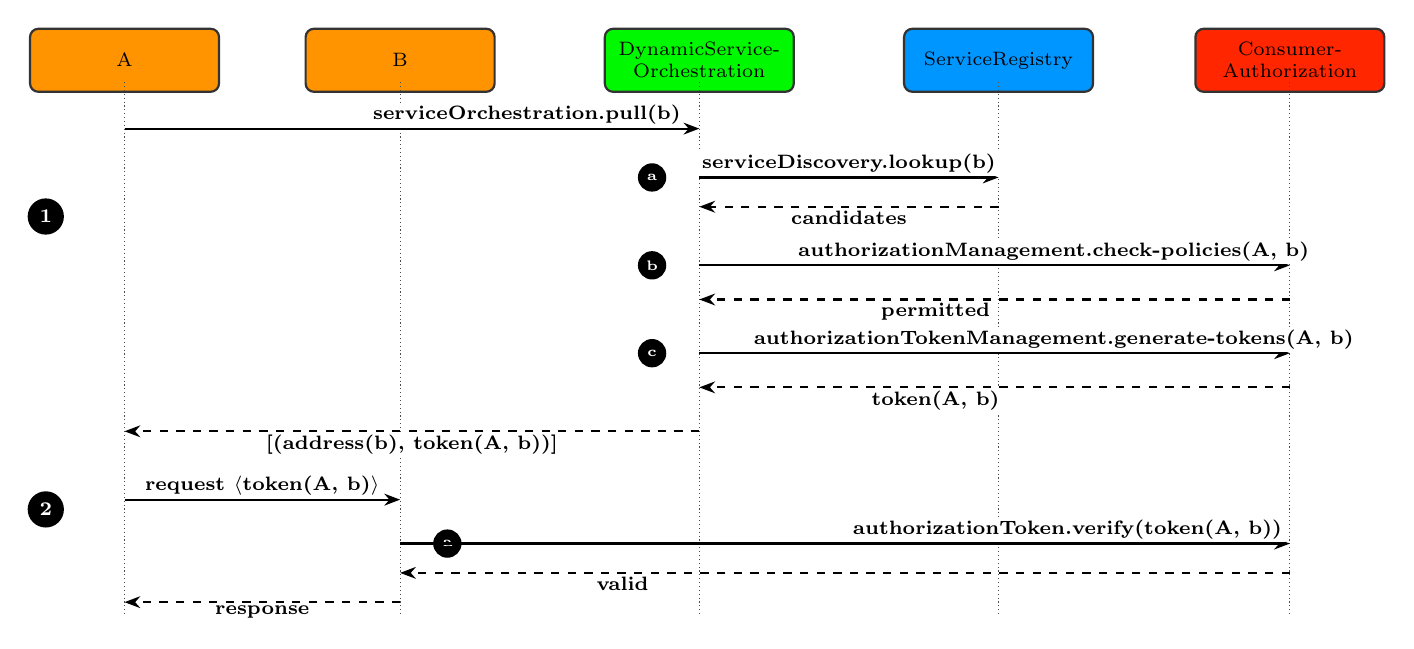
\begin{tikzpicture}[yscale=0.62]
  \seqhead{11.4}{0}{A}{fill=AppOrange, ahApplication}
  \seqhead{11.4}{3.5}{B}{fill=AppOrange, ahApplication}
  \seqhead{11.4}{7.3}{DynamicService-\\Orchestration}{fill=OrchGreen, ahOrchestration}
  \seqhead{11.4}{11.1}{ServiceRegistry}{fill=SRBlue, ahRegistry}
  \seqhead{11.4}{14.8}{Consumer-\\Authorization}{fill=AuthzRed, ahAuthorization}
  \node[num] at (-1.0,-3.2) {1};
  \draw[msg] (0,-1.4) -- node[lbl, above, pos=0.7]{serviceOrchestration.pull(b)} (7.3,-1.4);
  \node[sub] at (6.7,-2.4) {a};
  \draw[msg] (7.3,-2.4) -- node[lbl, above]{serviceDiscovery.lookup(b)} (11.1,-2.4);
  \draw[ret] (11.1,-3.0) -- node[lbl, below]{candidates} (7.3,-3.0);
  \node[sub] at (6.7,-4.2) {b};
  \draw[msg] (7.3,-4.2) -- node[lbl, above, pos=0.6]{authorizationManagement.check-policies(A, b)} (14.8,-4.2);
  \draw[ret] (14.8,-4.9) -- node[lbl, below, pos=0.6]{permitted} (7.3,-4.9);
  \node[sub] at (6.7,-6.0) {c};
  \draw[msg] (7.3,-6.0) -- node[lbl, above, pos=0.6]{authorizationTokenManagement.generate-tokens(A, b)} (14.8,-6.0);
  \draw[ret] (14.8,-6.7) -- node[lbl, below, pos=0.6]{token(A, b)} (7.3,-6.7);
  \draw[ret] (7.3,-7.6) -- node[lbl, below, pos=0.5]{[(address(b), token(A, b))]} (0,-7.6);
  \node[num] at (-1.0,-9.2) {2};
  \draw[msg] (0,-9.0) -- node[lbl, above]{request $\langle$token(A, b)$\rangle$} (3.5,-9.0);
  \node[sub] at (4.1,-9.9) {a};
  \draw[msg] (3.5,-9.9) -- node[lbl, above, pos=0.75]{authorizationToken.verify(token(A, b))} (14.8,-9.9);
  \draw[ret] (14.8,-10.5) -- node[lbl, below, pos=0.75]{valid} (3.5,-10.5);
  \draw[ret] (3.5,-11.1) -- node[lbl, below]{response} (0,-11.1);
\end{tikzpicture}
\caption{Authorisation and orchestration with access tokens.}
\label{fig:uc5}
\end{figure}

\begin{enumerate}
  \item A requests orchestration for \svc{b} from \sys{DynamicServiceOrchestration}, which
        responds with the network address of \svc{b} and the access token A needs to consume it.
        \begin{enumerate}[label=(\alph*)]
          \item The Orchestration system determines the candidate instances of \svc{b} by
                consulting the \sys{ServiceRegistry}.
          \item It checks with \sys{ConsumerAuthorization} which candidates A is permitted to
                consume, and removes the others.
          \item For the remaining candidates whose interface requires a token, it asks
                \sys{ConsumerAuthorization} to generate an access token for A. (The orchestration
                system is permitted to request tokens on behalf of consumers.)
        \end{enumerate}
  \item A consumes \svc{b} and includes the access token in the request. B responds.
        \begin{enumerate}[label=(\alph*)]
          \item Before responding, B verifies the token with \sys{ConsumerAuthorization}. A
                self-contained (signed) token can instead be verified locally with
                \sys{ConsumerAuthorization}'s public key.
        \end{enumerate}
\end{enumerate}
A is identified throughout by its certificate or identity token (Section~\ref{sec:uc:authn}).
In 5.0 the Orchestration system first checked whether A was authorised to request
orchestration; in 5.2.2 \svc{serviceOrchestration} is public to authenticated systems, and
authorisation is applied to the providers returned.

\subsection{Onboarding and Off-boarding}
\label{sec:uc:onboarding}

The onboarding process of the 5.0 Support GSoSD \cite{gsosdsup50} follows Bicaku et al.\
\cite{bicaku2018}: a new device proves that it is expected, obtains an identity from the system
that maintains identities, and registers its systems and services. Release 5.2.2 realises the
complete procedure, including off-boarding. The announcement steps of the 2018 procedure are
replaced by pre-distributed addresses (Section~\ref{sec:issues}), and identities are X.509
certificates of increasing scope: onboarding, device and system certificates.

\begin{figure}[h!]
\centering
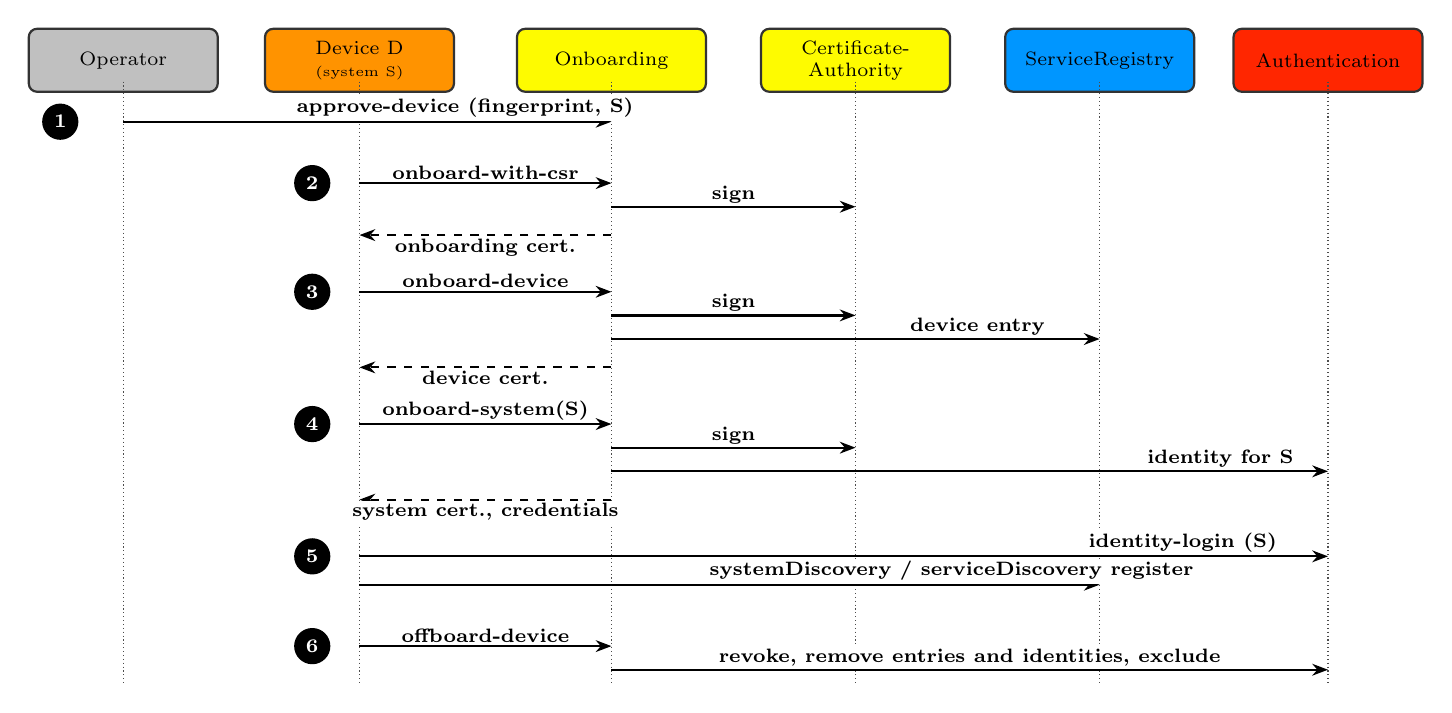
\begin{tikzpicture}[yscale=0.6]
  \seqhead{13.2}{0}{Operator}{fill=gray!15, ahInfrastructure}
  \seqhead{13.2}{3.0}{Device D\\{\tiny(system S)}}{fill=AppOrange, ahApplication}
  \seqhead{13.2}{6.2}{Onboarding}{fill=SupTeal, ahSupport}
  \seqhead{13.2}{9.3}{Certificate-\\Authority}{fill=SupTeal, ahSupport}
  \seqhead{13.2}{12.4}{ServiceRegistry}{fill=SRBlue, ahRegistry}
  \seqhead{13.2}{15.3}{Authentication}{fill=AuthnLilac, ahAuthentication}
  \node[num] at (-0.8,-1.3) {1};
  \draw[msg] (0,-1.3) -- node[lbl, above, pos=0.7]{approve-device (fingerprint, S)} (6.2,-1.3);
  \node[num] at (2.4,-2.6) {2};
  \draw[msg] (3.0,-2.6) -- node[lbl, above]{onboard-with-csr} (6.2,-2.6);
  \draw[msg] (6.2,-3.1) -- node[lbl, above]{sign} (9.3,-3.1);
  \draw[ret] (6.2,-3.7) -- node[lbl, below]{onboarding cert.} (3.0,-3.7);
  \node[num] at (2.4,-4.9) {3};
  \draw[msg] (3.0,-4.9) -- node[lbl, above]{onboard-device} (6.2,-4.9);
  \draw[msg] (6.2,-5.4) -- node[lbl, above]{sign} (9.3,-5.4);
  \draw[msg] (6.2,-5.9) -- node[lbl, above, pos=0.75]{device entry} (12.4,-5.9);
  \draw[ret] (6.2,-6.5) -- node[lbl, below]{device cert.} (3.0,-6.5);
  \node[num] at (2.4,-7.7) {4};
  \draw[msg] (3.0,-7.7) -- node[lbl, above]{onboard-system(S)} (6.2,-7.7);
  \draw[msg] (6.2,-8.2) -- node[lbl, above]{sign} (9.3,-8.2);
  \draw[msg] (6.2,-8.7) -- node[lbl, above, pos=0.85]{identity for S} (15.3,-8.7);
  \draw[ret] (6.2,-9.3) -- node[lbl, below]{system cert., credentials} (3.0,-9.3);
  \node[num] at (2.4,-10.5) {5};
  \draw[msg] (3.0,-10.5) -- node[lbl, above, pos=0.85]{identity-login (S)} (15.3,-10.5);
  \draw[msg] (3.0,-11.1) -- node[lbl, above, pos=0.8]{systemDiscovery / serviceDiscovery register} (12.4,-11.1);
  \node[num] at (2.4,-12.4) {6};
  \draw[msg] (3.0,-12.4) -- node[lbl, above]{offboard-device} (6.2,-12.4);
  \draw[msg] (6.2,-12.9) -- node[lbl, above, pos=0.5]{revoke, remove entries and identities, exclude} (15.3,-12.9);
\end{tikzpicture}
\caption{Onboarding and off-boarding of a device D hosting a system S (operations of
\svc{onboarding} and \svc{onboardingManagement}).}
\label{fig:uc6}
\end{figure}

\begin{enumerate}
  \item An operator approves device D: the fingerprint of its manufacturer-issued bootstrap
        certificate and the systems it may host, here S. Nothing that is not approved can enrol.
  \item D presents its bootstrap certificate and obtains a short-lived onboarding certificate
        (signed by the \sys{CertificateAuthority}) and the descriptions of the registry services.
  \item With the onboarding certificate D obtains its device certificate; the \sys{Onboarding}
        system registers D as a device in the \sys{ServiceRegistry}.
  \item With the device certificate D obtains, for each approved system, a system certificate and
        an identity in the \sys{Authentication} system.
  \item S logs in, registers itself (naming its device D) and its services, and from then on acts as
        any other system; what S may consume or provide is decided by access rules as usual.
  \item Off-boarding, requested by D or by the operator, withdraws everything: certificates are
        revoked, registry entries and identities removed, and S is excluded through the
        \sys{Blacklist}.
\end{enumerate}
Each step accepts only the credential issued in the previous step, and only the latest valid one; a
superseded or revoked credential is refused.


\paragraph{PDE backend update, 23 October 2026.} The Java PDE now submits its complete engineered
plant to DynamicServiceOrchestration, which constrains each managed consumer/service to
eligible engineered providers and their priorities. An unavailable producer yields no
result rather than an unrelated provider. Admission and service-authorisation requirements
still apply. SSO remains optional and is no longer required by PDE. The white-box GSoSDDs
specify the local extension and coordinated upgrade; existing consumer caches may delay
visible changes. This records implementation changes, not proof of a new live deployment.

\subsection{Plant-Description-Driven Orchestration}
\label{sec:uc:pde}

An engineer describes the connections of a plant in the engineering UI (Section~\ref{sec:mgmt})
and lets the \sys{PlantDescriptionEngine} turn them into orchestration rules. We assume all
systems are registered and monitored.

\begin{figure}[h!]
\centering
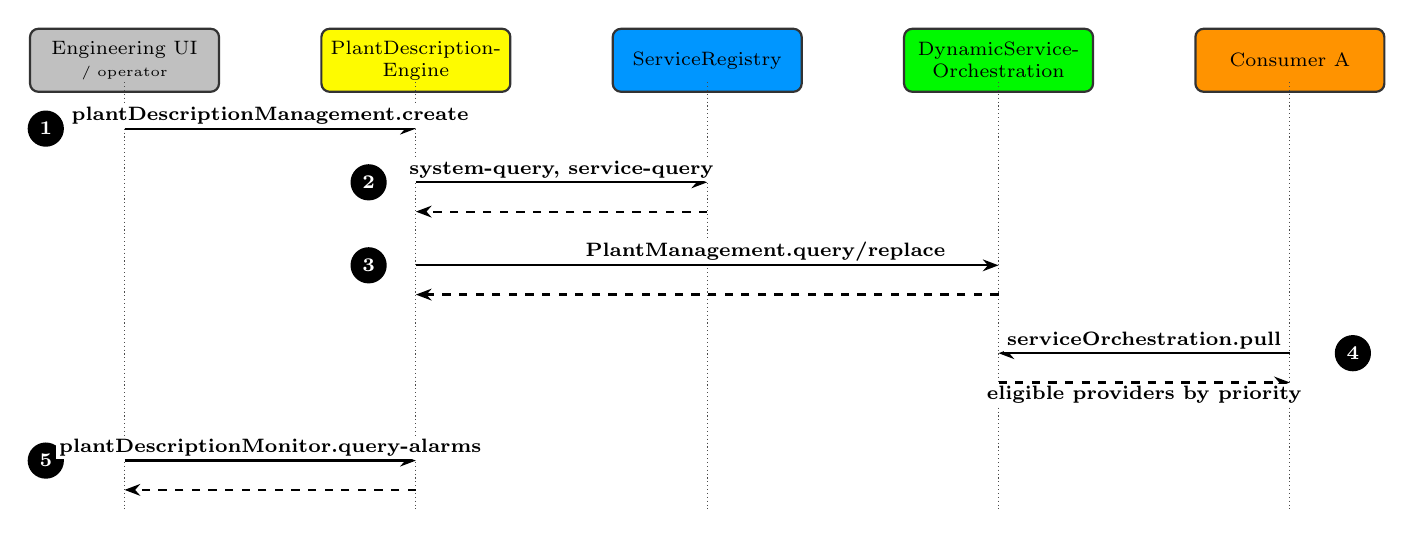
\begin{tikzpicture}[yscale=0.62]
  \seqhead{9.2}{0}{Engineering UI\\{\tiny / operator}}{fill=gray!15, ahInfrastructure}
  \seqhead{9.2}{3.7}{PlantDescription-\\Engine}{fill=SupTeal, ahSupport}
  \seqhead{9.2}{7.4}{ServiceRegistry}{fill=SRBlue, ahRegistry}
  \seqhead{9.2}{11.1}{DynamicService-\\Orchestration}{fill=OrchGreen, ahOrchestration}
  \seqhead{9.2}{14.8}{Consumer A}{fill=AppOrange, ahApplication}
  \node[num] at (-1.0,-1.4) {1};
  \draw[msg] (0,-1.4) -- node[lbl, above]{plantDescriptionManagement.create} (3.7,-1.4);
  \node[num] at (3.1,-2.5) {2};
  \draw[msg] (3.7,-2.5) -- node[lbl, above]{system-query, service-query} (7.4,-2.5);
  \draw[ret] (7.4,-3.1) -- (3.7,-3.1);
  \node[num] at (3.1,-4.2) {3};
  \draw[msg] (3.7,-4.2) -- node[lbl, above, pos=0.6]{PlantManagement.query/replace} (11.1,-4.2);
  \draw[ret] (11.1,-4.8) -- (3.7,-4.8);
  \node[num] at (15.6,-6.0) {4};
  \draw[msg] (14.8,-6.0) -- node[lbl, above]{serviceOrchestration.pull} (11.1,-6.0);
  \draw[ret] (11.1,-6.6) -- node[lbl, below]{eligible providers by priority} (14.8,-6.6);
  \node[num] at (-1.0,-8.2) {5};
  \draw[msg] (0,-8.2) -- node[lbl, above]{plantDescriptionMonitor.query-alarms} (3.7,-8.2);
  \draw[ret] (3.7,-8.8) -- (0,-8.8);
\end{tikzpicture}
\caption{Plant-description-driven orchestration.}
\label{fig:uc7}
\end{figure}

\begin{enumerate}
  \item The engineer creates and activates a plant description in the engineering UI, which
        stores it with the \sys{PlantDescriptionEngine}.
  \item The \sys{PlantDescriptionEngine} matches the described systems with the registered ones.
  \item It atomically replaces the managed consumer/service scopes and provider priorities
        for the active plant; unavailable producers retain empty scopes. Steps 2--3 repeat periodically and after
        every change.
  \item A consumer obtains its orchestration from DynamicServiceOrchestration as in
        the dynamic-orchestration contract; authorisation and eligibility checks still apply.
  \item The operator reads the alarms raised for deviations between the plant and its
        description, including systems without recent monitoring observations.
\end{enumerate}
The engineer stays in control of the plant's composition: changing the description in the UI
changes DSO's managed snapshot within one successful synchronisation interval. Consumer
orchestration caches may delay visible changes; no consumer reconfiguration is required.

\subsection{Workflow Execution}
\label{sec:uc:choreo}

A client runs a workflow plan. We assume the plan and its executors are registered with the
\sys{Choreographer}, and that access rules exist for the executors on the step services.

\begin{figure}[h!]
\centering
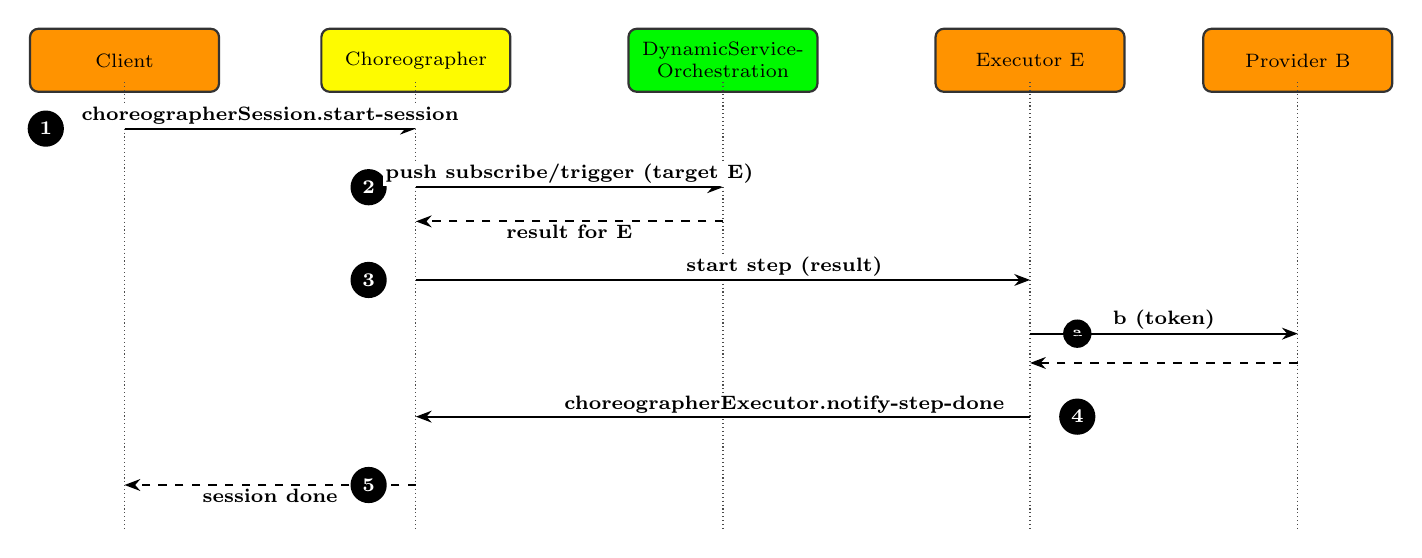
\begin{tikzpicture}[yscale=0.62]
  \seqhead{9.6}{0}{Client}{fill=AppOrange, ahApplication}
  \seqhead{9.6}{3.7}{Choreographer}{fill=SupTeal, ahSupport}
  \seqhead{9.6}{7.6}{DynamicService-\\Orchestration}{fill=OrchGreen, ahOrchestration}
  \seqhead{9.6}{11.5}{Executor E}{fill=AppOrange, ahApplication}
  \seqhead{9.6}{14.9}{Provider B}{fill=AppOrange, ahApplication}
  \node[num] at (-1.0,-1.4) {1};
  \draw[msg] (0,-1.4) -- node[lbl, above]{choreographerSession.start-session} (3.7,-1.4);
  \node[num] at (3.1,-2.6) {2};
  \draw[msg] (3.7,-2.6) -- node[lbl, above]{push subscribe/trigger (target E)} (7.6,-2.6);
  \draw[ret] (7.6,-3.3) -- node[lbl, below]{result for E} (3.7,-3.3);
  \node[num] at (3.1,-4.5) {3};
  \draw[msg] (3.7,-4.5) -- node[lbl, above, pos=0.6]{start step (result)} (11.5,-4.5);
  \node[sub] at (12.1,-5.6) {a};
  \draw[msg] (11.5,-5.6) -- node[lbl, above]{b (token)} (14.9,-5.6);
  \draw[ret] (14.9,-6.2) -- (11.5,-6.2);
  \node[num] at (12.1,-7.3) {4};
  \draw[msg] (11.5,-7.3) -- node[lbl, above, pos=0.4]{choreographerExecutor.notify-step-done} (3.7,-7.3);
  \node[num] at (3.1,-8.7) {5};
  \draw[ret] (3.7,-8.7) -- node[lbl, below]{session done} (0,-8.7);
\end{tikzpicture}
\caption{Execution of one workflow step.}
\label{fig:uc8}
\end{figure}

\begin{enumerate}
  \item The client starts a session of a plan.
  \item For each step ready to run, the \sys{Choreographer} selects an executor E and has the
        advanced Orchestration system orchestrate the step's service requirement for E; the
        result, including tokens issued to E, is pushed back.
  \item The \sys{Choreographer} starts E with the orchestration result.
        \begin{enumerate}[label=(\alph*)]
          \item E consumes the provider's service with its own identity and token.
        \end{enumerate}
  \item E reports the step result; on error the step is retried with another executor.
  \item When all actions and iterations are done, the session ends.
\end{enumerate}

\subsection{Orchestration with Translation}
\label{sec:uc:translation}

Consumer A requires a service that is only provided with an interface or data model A cannot use.
Translation is enabled in the advanced Orchestration system and allowed in A's request.

\begin{figure}[h!]
\centering
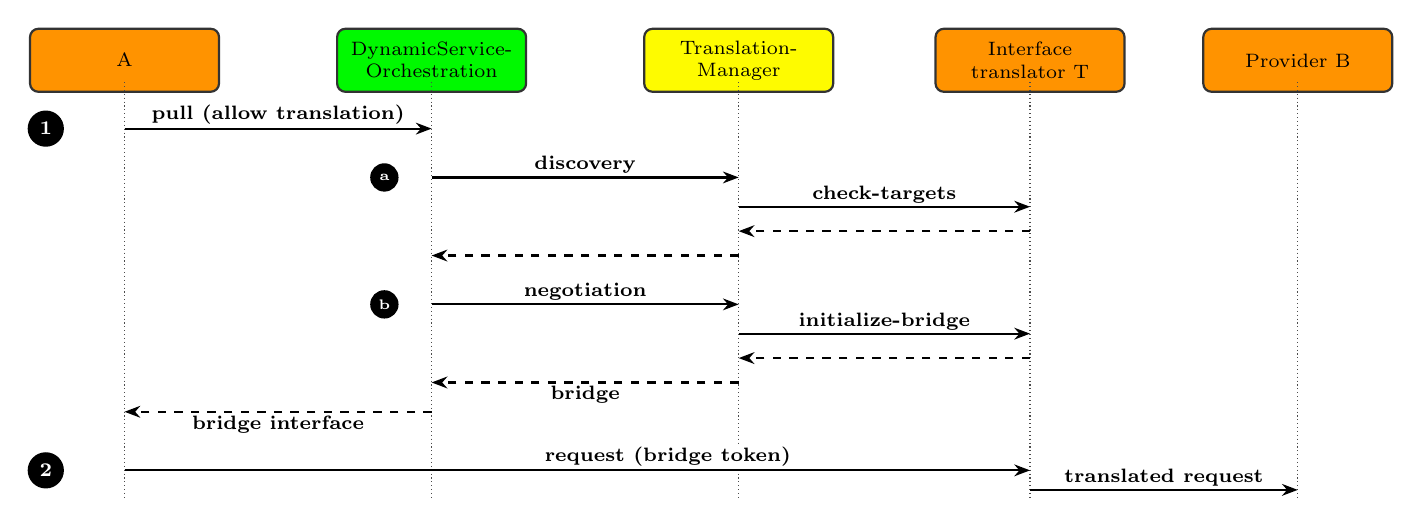
\begin{tikzpicture}[yscale=0.62]
  \seqhead{9.0}{0}{A}{fill=AppOrange, ahApplication}
  \seqhead{9.0}{3.9}{DynamicService-\\Orchestration}{fill=OrchGreen, ahOrchestration}
  \seqhead{9.0}{7.8}{Translation-\\Manager}{fill=SupTeal, ahSupport}
  \seqhead{9.0}{11.5}{Interface\\translator T}{fill=gray!15, ahApplication}
  \seqhead{9.0}{14.9}{Provider B}{fill=AppOrange, ahApplication}
  \node[num] at (-1.0,-1.4) {1};
  \draw[msg] (0,-1.4) -- node[lbl, above]{pull (allow translation)} (3.9,-1.4);
  \node[sub] at (3.3,-2.4) {a};
  \draw[msg] (3.9,-2.4) -- node[lbl, above]{discovery} (7.8,-2.4);
  \draw[msg] (7.8,-3.0) -- node[lbl, above]{check-targets} (11.5,-3.0);
  \draw[ret] (11.5,-3.5) -- (7.8,-3.5);
  \draw[ret] (7.8,-4.0) -- (3.9,-4.0);
  \node[sub] at (3.3,-5.0) {b};
  \draw[msg] (3.9,-5.0) -- node[lbl, above]{negotiation} (7.8,-5.0);
  \draw[msg] (7.8,-5.6) -- node[lbl, above]{initialize-bridge} (11.5,-5.6);
  \draw[ret] (11.5,-6.1) -- (7.8,-6.1);
  \draw[ret] (7.8,-6.6) -- node[lbl, below]{bridge} (3.9,-6.6);
  \draw[ret] (3.9,-7.2) -- node[lbl, below]{bridge interface} (0,-7.2);
  \node[num] at (-1.0,-8.4) {2};
  \draw[msg] (0,-8.4) -- node[lbl, above, pos=0.6]{request (bridge token)} (11.5,-8.4);
  \draw[msg] (11.5,-8.8) -- node[lbl, above]{translated request} (14.9,-8.8);
\end{tikzpicture}
\caption{Orchestration with an interface translation bridge (responses omitted in step 2).}
\label{fig:uc9}
\end{figure}

\begin{enumerate}
  \item A requests orchestration and allows translation. No provider is directly compatible.
        \begin{enumerate}[label=(\alph*)]
          \item The Orchestration system asks the \sys{TranslationManager} to discover possible
                bridges; it asks interface translators which candidate providers they can reach
                and, if needed, finds data model translators.
          \item The Orchestration system selects a candidate and asks the \sys{TranslationManager}
                to negotiate the bridge, which initialises it in the translator and returns the
                bridge interface, protected by a bridge token.
        \end{enumerate}
  \item A consumes the bridge interface like a normal service; the translator forwards translated
        requests to B and reports usage to the \sys{TranslationManager}.
\end{enumerate}

\subsection{Event-Driven Communication}
\label{sec:uc:events}

\begin{figure}[h!]
\centering
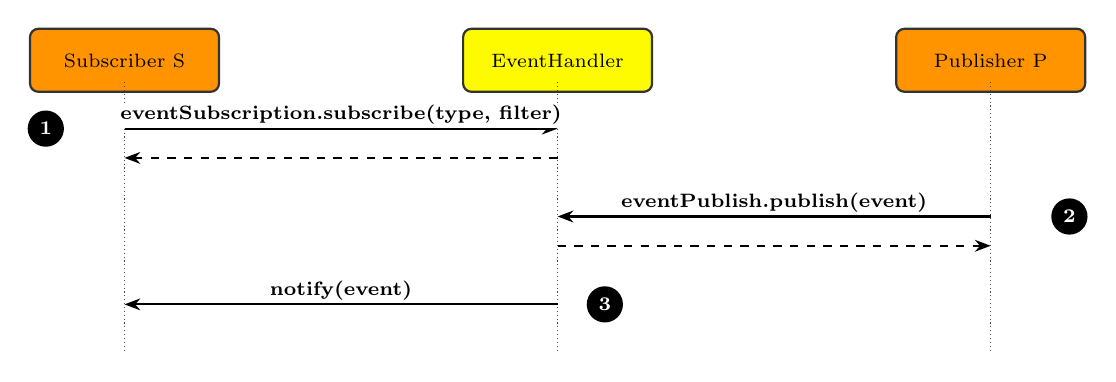
\begin{tikzpicture}[yscale=0.62]
  \seqhead{6.0}{0}{Subscriber S}{fill=AppOrange, ahApplication}
  \seqhead{6.0}{5.5}{EventHandler}{fill=SupTeal, ahSupport}
  \seqhead{6.0}{11}{Publisher P}{fill=AppOrange, ahApplication}
  \node[num] at (-1.0,-1.4) {1};
  \draw[msg] (0,-1.4) -- node[lbl, above]{eventSubscription.subscribe(type, filter)} (5.5,-1.4);
  \draw[ret] (5.5,-2.0) -- (0,-2.0);
  \node[num] at (12.0,-3.2) {2};
  \draw[msg] (11,-3.2) -- node[lbl, above]{eventPublish.publish(event)} (5.5,-3.2);
  \draw[ret] (5.5,-3.8) -- (11,-3.8);
  \node[num] at (6.1,-5.0) {3};
  \draw[msg] (5.5,-5.0) -- node[lbl, above]{notify(event)} (0,-5.0);
\end{tikzpicture}
\caption{Event-driven communication.}
\label{fig:uc10}
\end{figure}

\begin{enumerate}
  \item S subscribes to an event type with an optional metadata filter, validity window and
        notification address.
  \item P publishes an event; its identity is taken from authentication.
  \item The \sys{EventHandler} delivers the event to every subscriber whose filter and validity
        window match.
\end{enumerate}
Publisher and subscribers never need to know each other. Access control on event types is an open
issue (Section~\ref{sec:issues}).

\subsection{Monitoring of the Local Cloud}
\label{sec:uc:monitoring}

\begin{figure}[h!]
\centering
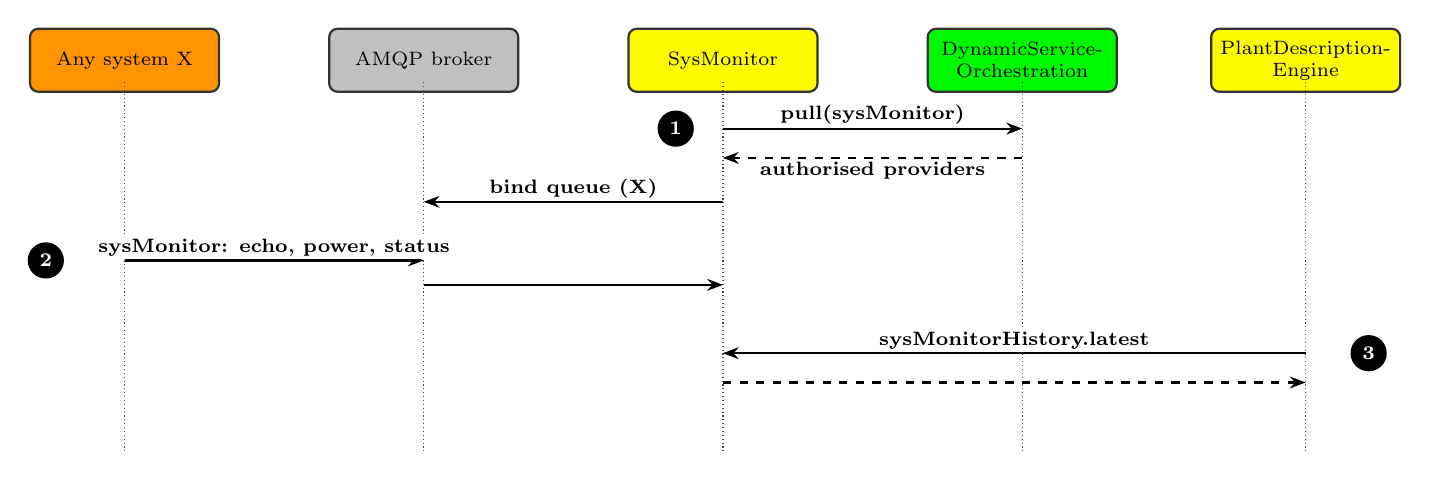
\begin{tikzpicture}[yscale=0.62]
  \seqhead{8.0}{0}{Any system X}{fill=AppOrange, ahApplication}
  \seqhead{8.0}{3.8}{AMQP broker}{fill=gray!15, ahInfrastructure}
  \seqhead{8.0}{7.6}{SysMonitor}{fill=SupTeal, ahSupport}
  \seqhead{8.0}{11.4}{DynamicService-\\Orchestration}{fill=OrchGreen, ahOrchestration}
  \seqhead{8.0}{15.0}{PlantDescription-\\Engine}{fill=SupTeal, ahSupport}
  \node[num] at (7.0,-1.4) {1};
  \draw[msg] (7.6,-1.4) -- node[lbl, above]{pull(sysMonitor)} (11.4,-1.4);
  \draw[ret] (11.4,-2.0) -- node[lbl, below]{authorised providers} (7.6,-2.0);
  \draw[msg] (7.6,-2.9) -- node[lbl, above]{bind queue (X)} (3.8,-2.9);
  \node[num] at (-1.0,-4.1) {2};
  \draw[msg] (0,-4.1) -- node[lbl, above]{sysMonitor: echo, power, status} (3.8,-4.1);
  \draw[msg] (3.8,-4.6) -- (7.6,-4.6);
  \node[num] at (15.8,-6.0) {3};
  \draw[msg] (15.0,-6.0) -- node[lbl, above]{sysMonitorHistory.latest} (7.6,-6.0);
  \draw[ret] (7.6,-6.6) -- (15.0,-6.6);
\end{tikzpicture}
\caption{Monitoring of the local cloud.}
\label{fig:uc11}
\end{figure}

\begin{enumerate}
  \item The \sys{SysMonitor} obtains the \svc{sysMonitor} providers it is authorised for through
        orchestration and binds its queue at the AMQP broker to their observations.
  \item Every system X publishes its observations periodically to the AMQP broker; the
        \sys{SysMonitor} receives, validates and stores them, and republishes them in normalised
        form over MQTT (\svc{sysMonitorData}).
  \item Consumers such as the \sys{PlantDescriptionEngine} read the history to detect systems that
        are degraded, not monitored or silent.
\end{enumerate}

\subsection{Inter-Cloud Service Consumption}
\label{sec:uc:intercloud}

Consumer A in local cloud 1 needs a service \svc{b} that only provider B in local cloud 2 offers. Both
clouds belong to the same organisation and are connected by an inter-cloud relay
(Section~\ref{sec:sup:relay}); cloud 2 has granted A of cloud 1 access to \svc{b}.

\begin{figure}[h!]
\centering
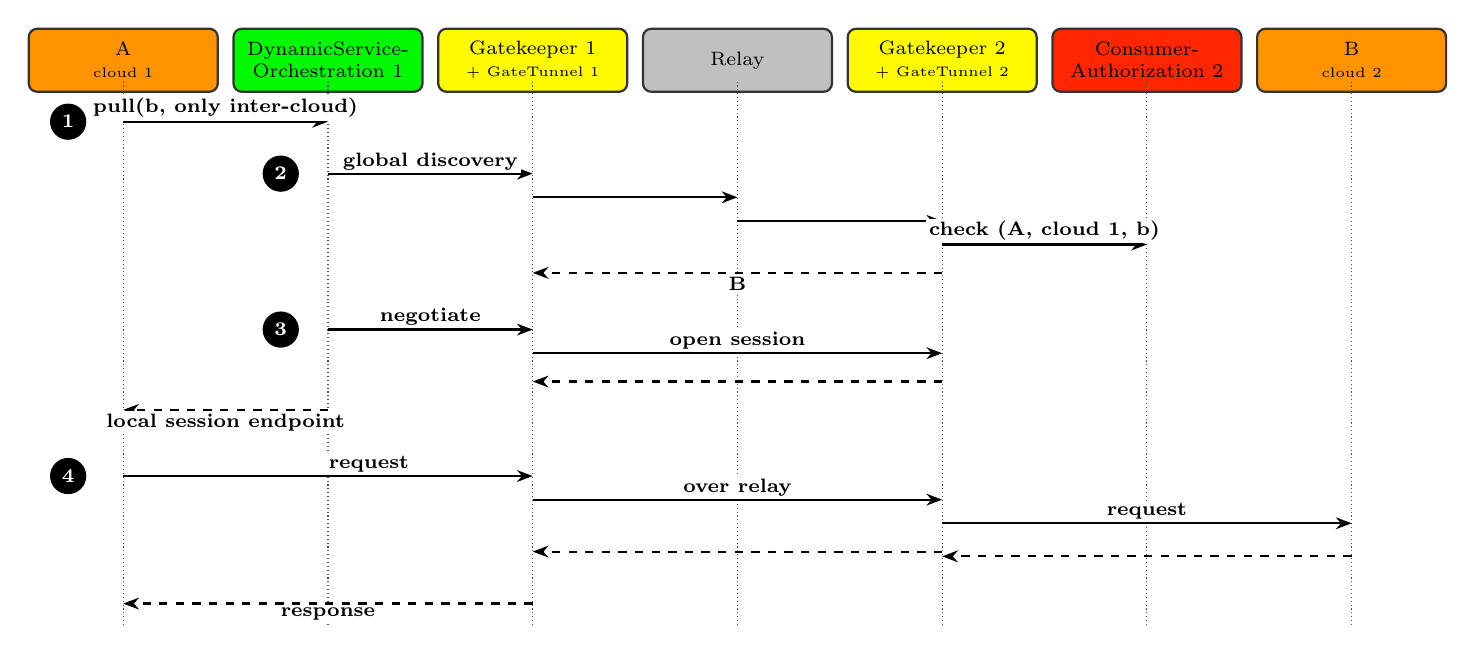
\begin{tikzpicture}[yscale=0.6]
  \seqhead{12.0}{0}{A\\{\tiny cloud 1}}{fill=AppOrange, ahApplication}
  \seqhead{12.0}{2.6}{DynamicService-\\Orchestration 1}{fill=OrchGreen, ahOrchestration}
  \seqhead{12.0}{5.2}{Gatekeeper 1\\{\tiny + GateTunnel 1}}{fill=SupTeal, ahSupport}
  \seqhead{12.0}{7.8}{Relay}{fill=gray!15, ahInfrastructure}
  \seqhead{12.0}{10.4}{Gatekeeper 2\\{\tiny + GateTunnel 2}}{fill=SupTeal, ahSupport}
  \seqhead{12.0}{13.0}{Consumer-\\Authorization 2}{fill=AuthzRed, ahAuthorization}
  \seqhead{12.0}{15.6}{B\\{\tiny cloud 2}}{fill=AppOrange, ahApplication}
  \node[num] at (-0.7,-1.3) {1};
  \draw[msg] (0,-1.3) -- node[lbl, above]{pull(b, only inter-cloud)} (2.6,-1.3);
  \node[num] at (2.0,-2.4) {2};
  \draw[msg] (2.6,-2.4) -- node[lbl, above]{global discovery} (5.2,-2.4);
  \draw[msg] (5.2,-2.9) -- (7.8,-2.9);
  \draw[msg] (7.8,-3.4) -- (10.4,-3.4);
  \draw[msg] (10.4,-3.9) -- node[lbl, above]{check (A, cloud 1, b)} (13.0,-3.9);
  \draw[ret] (10.4,-4.5) -- node[lbl, below]{B} (5.2,-4.5);
  \node[num] at (2.0,-5.7) {3};
  \draw[msg] (2.6,-5.7) -- node[lbl, above]{negotiate} (5.2,-5.7);
  \draw[msg] (5.2,-6.2) -- node[lbl, above]{open session} (10.4,-6.2);
  \draw[ret] (10.4,-6.8) -- (5.2,-6.8);
  \draw[ret] (2.6,-7.4) -- node[lbl, below]{local session endpoint} (0,-7.4);
  \node[num] at (-0.7,-8.8) {4};
  \draw[msg] (0,-8.8) -- node[lbl, above, pos=0.6]{request} (5.2,-8.8);
  \draw[msg] (5.2,-9.3) -- node[lbl, above]{over relay} (10.4,-9.3);
  \draw[msg] (10.4,-9.8) -- node[lbl, above, pos=0.5]{request} (15.6,-9.8);
  \draw[ret] (15.6,-10.5) -- (10.4,-10.5);
  \draw[ret] (10.4,-10.4) -- (5.2,-10.4);
  \draw[ret] (5.2,-11.5) -- node[lbl, below]{response} (0,-11.5);
\end{tikzpicture}
\caption{Inter-cloud service consumption through Gatekeepers, GateTunnels and the relay.}
\label{fig:uc12}
\end{figure}

\begin{enumerate}
  \item A requests orchestration for \svc{b}, allowing or requiring providers in other clouds.
  \item The advanced Orchestration system of cloud 1 asks its \sys{Gatekeeper} for a global service
        discovery. The request reaches the \sys{Gatekeeper} of cloud 2 over the relay; it looks
        \svc{b} up in its own registry and keeps only the providers its Authorisation system grants
        to A of cloud 1.
  \item The Orchestration system has its \sys{Gatekeeper} negotiate access to B. The provider's
        \sys{Gatekeeper} checks authorisation again; both \sys{Gatekeeper}s have their
        \sys{GateTunnel}s open the two ends of a session. The orchestration result given to A is
        the local session endpoint of \sys{GateTunnel} 1.
  \item A consumes \svc{b} at that endpoint with its own credentials, as it would a local
        provider. \sys{GateTunnel} 1 forwards the request over the relay; \sys{GateTunnel} 2
        accepts it only from its negotiated peer and only for B's service, calls B and returns the
        response.
\end{enumerate}
No system of cloud 1 needs credentials of cloud 2, and neither cloud exposes its internal network:
both clouds connect outwards to the relay.

\newpage
%% ============================================================================================
\section{Control and Data Planes}
\label{sec:planes}

None of the Core and Support systems provided by the Eclipse Arrowhead project are designed to
directly fulfil the business objectives of any given local cloud. What they are designed to do
is to help create the situation in which these business objectives can be fulfilled. They do
this, generally, by controlling and distributing information about the local cloud and its
resources.

Traditionally, computer networks are reasoned about in planes, where each plane presents the
same network from a different perspective with its own aims and conditions. The term
\emph{control plane} is used when considering how networking equipment, such as firewalls,
switches and routers, is set up to allow information to flow in certain ways. The term
\emph{data plane} is used when considering the contents of those information flows, without
regard to how they were set up. This separation increases the number of things that must be
considered, but reduces the complexity of each of them.

In a similar manner, we use the term control plane when considering how systems are controlled
to facilitate desired service consumption patterns. In a control-plane diagram, interactions
between Core, Support and application systems are illustrated, but communication between
application systems is left out. The reverse holds for data-plane diagrams. In this document we
do not separate the two: while we focus on the control plane, the data plane is included for
clarity. In Figure~\ref{fig:uc5}, message exchange 1 is exclusively concerned with the control
plane: A obtains the control-plane details needed to consume \svc{b}. Exchange 2a also belongs
to the control plane, as it is between a Core system and an application system. A pure
data-plane version would only include the request and response between A and B, without
any reference to tokens.

An important aspect of the control plane is that no application data exchange occurs there. The
Core systems should not have to consider the requirements of the data transmissions in an
Arrowhead local cloud. Cached orchestration and locally verifiable tokens can reduce
control-plane traffic while valid credentials, authorisation decisions and encrypted
channels remain enforceable. They do not justify shutting down AAA dependencies
that a provider still needs for identity, permission, token or revocation checks.
An unavailable required check fails closed. Control/data-plane separation permits
different performance and scaling without removing the v5.0 security baseline.

Support systems can be placed in the same way. The orchestration-support systems,
\sys{PlantDescriptionEngine}, \sys{Choreographer}, \sys{CertificateAuthority}, \sys{Onboarding},
\sys{Configuration}, \sys{SysMonitor} and \sys{Gatekeeper} belong to the control plane: they decide
or prepare who talks to whom, with which credentials and settings, and observe the result.
\sys{EventHandler}, \sys{DataManager} and \sys{TimeManager} provide application-level services and
belong to the data plane. Translation bridges and \sys{GateTunnel} sessions are set up in the control
plane but carry data-plane traffic; their capacity must therefore be planned with the data plane.
Above the control plane, the \sys{PlantDescriptionEngine} and its engineering UI form a
management layer that states how the control plane shall configure the local cloud
(Section~\ref{sec:mgmt}).

When designing a local cloud, it is generally useful to split the design into a control and a
data plane. The first is concerned with which Core and Support systems, as well as other
complementary systems, are used and under what conditions. The second is concerned with how
the local cloud directly addresses its business objectives.

%% ============================================================================================




% \subsection{Deployed Java Reference Cloud (24 October 2026)}
% \label{sec:java-deployment}
% The Java reference deployment is the Docker Compose project
% \prop{arrowhead-v52-test-cloud}, maintained in \prop{Arrowhead-test-cloud-java}.
% Figure~\ref{fig:java-deployment} records its 22 deployed microsystems, including
% both orchestration variants, the operations manager and the demonstration application
% \cite{javaDeployment20261024}. This is a dated deployment example of the architecture,
% not a requirement that every local cloud deploy every optional support system.
% In this 24 October snapshot, the five Core systems and fifteen support systems
% are Java implementations;
% \sys{LocalCloudManager} has a Node.js API and \sys{RandomDataProducer} is a Python
% application. Thus ``Java cloud'' identifies the reference implementation baseline,
% not the language of every process.

% \begin{figure}[htbp]
% \centering
% % Deployment snapshot, 24 October 2026. Editable vector artwork.
\begin{tikzpicture}[x=1cm,y=1cm,
  block/.style={draw=ArrowheadBlue,fill=ArrowheadBlue!4,rounded corners=2pt,
  text width=3.55cm,align=center,font=\scriptsize,inner sep=4pt},
  route/.style={-{Stealth[length=2mm]},thick,ArrowheadBlue}]
\node[block,text width=15.3cm,minimum height=0.9cm, ahMixed] (bus) at (6,0)
 {\textbf{Common service-consumption contract}\\
 ServiceRegistry discovery $\rightarrow$ Authentication identity $\rightarrow$
 service orchestration $\rightarrow$ direct, authorised provider call};
\node[block,anchor=north,minimum height=5.4cm, ahMixed] (core) at (0,-1.1)
 {\textbf{Core (5; private owned state)}\\[5pt]
 \colorbox{AHSysMLRegistry}{\parbox{3.1cm}{\centering ServiceRegistry}}\\[4pt]
 \colorbox{AHSysMLSecurity}{\parbox{3.1cm}{\centering Authentication}}\\[4pt]
 \colorbox{AHSysMLSecurity}{\parbox{3.1cm}{\centering ConsumerAuthorization}}\\[4pt]
 \colorbox{AHSysMLOrchestration}{\parbox{3.1cm}{\centering DynamicService-\\Orchestration}}\\[4pt]
 \colorbox{AHSysMLOrchestration}{\parbox{3.1cm}{\centering SimpleStoreService-\\Orchestration}}};
\node[block,anchor=north,minimum height=5.4cm, ahSupport] (life) at (4,-1.1)
 {\textbf{Lifecycle and policy (4)}\\[5pt]
 Blacklist\\[7pt] Onboarding\\[7pt] CertificateAuthority\\[7pt] DeviceQoSEvaluator};
\node[block,anchor=north,minimum height=5.4cm, ahSupport] (svc) at (8,-1.1)
 {\textbf{Data and engineering (7)}\\[5pt]
 TranslationManager\\[4pt] DataManager\\[4pt] TimeManager\\[4pt] EventHandler\\[4pt]
 Configuration\\[4pt] PlantDescriptionEngine\\[4pt] Choreographer};
\node[block,anchor=north,minimum height=5.4cm, ahMixed] (ops) at (12,-1.1)
 {\textbf{Operations and exchange (6)}\\[5pt]
 \colorbox{AHSysMLSupport}{\strut SysMonitor}\\[4pt] \colorbox{AHSysMLSupport}{\strut AIGym}\\[4pt] \colorbox{AHSysMLSupport}{\strut Gatekeeper}\\[4pt] \colorbox{AHSysMLSupport}{\strut GateTunnel}\\[4pt]
 \colorbox{AHSysMLSupport}{\strut LocalCloudManager}\\[4pt]\colorbox{AHSysMLApplication}{\strut RandomDataProducer}};
\foreach \n in {core,life,svc,ops} \draw[route] (bus.south -| \n.north) -- (\n.north);
\node[block,text width=15.3cm,minimum height=1cm, ahMixed] (monitor) at (6,-7.5)
 {\textbf{Native monitoring from all 22 microsystems}\\
 AMQP broker $\rightarrow$ SysMonitor (SQLite history/outbox)
 $\rightarrow$ MQTT broker $\rightarrow$ AIGym};
\draw[route] (ops.south) -- (ops.south |- monitor.north);
\node[block,text width=15.3cm,fill=gray!6,draw=ArrowheadGrey, ahInfrastructure] at (6,-9)
 {\textbf{Integrated assets:} 15 private MySQL containers owned by their microsystems.\\
 \textbf{Infrastructure:} AMQP and MQTT brokers; dashboard UI; constrained Docker proxy.\\
 24 October snapshot: 41 containers. The federation relay is a separate project.};
\end{tikzpicture}

% \caption{Deployed Java reference cloud. All 22 named systems are microsystems;
% message brokers, dashboard and Docker proxy are infrastructure; database
% containers are integrated assets inside their host microsystems.
% The shared consumption path is drawn once to avoid repeating bootstrap edges.}
% \label{fig:java-deployment}
% \end{figure}
% \FloatBarrier

% The 41 running containers comprise the 22 microsystems, 15 dedicated MySQL
% containers, two message brokers, a dashboard UI and a Docker proxy. The four
% \sys{CertificateAuthority}, \sys{Gatekeeper}, \sys{GateTunnel} and \sys{SysMonitor}
% services originally used the combined Java 21 runtime in this dated snapshot.
% The primary distribution now packages each as an independent Java 21 project
% with its own SQLite state; this source change is not a blanket live-image rollout.
% The former delegated \sys{SysMonitorPublisher} is not a deployed microsystem:
% each system publishes its own \svc{sysMonitor} observations.

% \paragraph{Discovery, orchestration and direct consumption.}
% Systems bootstrap through \sys{ServiceRegistry}, locate \svc{identity} and
% \svc{serviceOrchestration}, obtain a certificate-bound identity token and request
% an authorised provider for the required operation. The resulting call goes from
% consumer to provider; the orchestrator does not proxy the application payload.
% DSO directly discovers its own authorisation and blacklist dependencies to avoid
% recursive orchestration. Authentication also bootstraps its authorisation check.
% Other dependency calls use orchestration, with the documented caches and exceptions.

% \paragraph{Monitoring and application data.}
% Native publishers send observations over AMQPS to RabbitMQ; \sys{SysMonitor}
% consumes authorised selections and stores them in its own SQLite history/outbox.
% It republishes normalised \svc{sysMonitorData} through MQTT for \sys{AIGym}.
% \sys{LocalCloudManager} reads \svc{sysMonitorHistory} and manages subscriptions.
% The demonstration producer instead writes application SenML data to
% \sys{DataManager} every 30\,s through \svc{dataHistorian}~\op{put-data}.
% Monitoring history is not stored by DataManager.

% \paragraph{Engineering, workflow and federation paths.}
% The plant editor calls \sys{PlantDescriptionEngine}; an active plant is compiled
% into an atomic DSO rule snapshot through \svc{serviceOrchestrationPlantManagement}.
% \sys{Choreographer} asks DSO for push orchestration on behalf of workflow executors;
% no executor is deployed by default. Onboarding consumes certificate signing,
% validation and revocation, identity management and blacklist operations.
% Inter-cloud selection uses Gatekeeper discovery/negotiation and an AH-GT-1
% GateTunnel session over the external relay. The 24 October deployment snapshot contained
% neither SimpleStore route rows nor an active DSO plant-rule row: these mechanisms
% are available, but the diagram does not imply an active engineered workflow.

% \paragraph{Reference security profile.}
% The deployed service profile realises the v5.0-and-later default: full AAA and
% information encryption, using mutual TLS with \texttt{CERT\_AUTH}, certificate-bound
% identity tokens and operation-scoped authorisation. Unsecured component samples
% are explicit development exceptions, not an alternative architectural default. The operator console requires login and reaches
% Docker only through a project-scoped proxy. CertificateAuthority publishes CRLs;
% services and brokers enforce them on new TLS handshakes. Ending established
% connections is a separate action. AH-GT-1 protects relayed payloads end to end;
% cloud application trust remains separate from relay/organisation trust
% \cite{javaDeployment20261024,rustFederation20261019}.

% \subsection{Principal Deployed Service Paths}
% Figure~\ref{fig:java-service-paths} distinguishes the orchestration decision from
% the subsequent application call and relates the main optional management and
% federation services to that path.
% \begin{figure}[htbp]
% \centering
% % Main service paths; arrows show service/data direction, not a traffic trace.
\begin{tikzpicture}[x=1cm,y=1cm,
 b/.style={draw=ArrowheadBlue,fill=ArrowheadBlue!4,rounded corners=2pt,
 text width=4.2cm,align=center,font=\scriptsize,minimum height=0.95cm},
 a/.style={-{Stealth[length=2mm]},thick,ArrowheadBlue},
 t/.style={font=\scriptsize,fill=white,align=center,text width=3.8cm,inner sep=2pt}]
\node[b, ahApplication] (rdp) at (0,0) {RandomDataProducer};
\node[b, ahOrchestration] (dso) at (5.3,0) {DynamicServiceOrchestration};
\node[b, ahSupport] (dm) at (10.6,0) {DataManager\\dataHistorian / dataProxy};
\draw[a] (rdp) -- node[t,below=18pt]{service requirement} (dso);
\draw[a,dashed] (dso) -- node[t,above=18pt]{discovers / selects provider} (dm);
\draw[a] (dso.north west) to[bend right=40] node[t,above=2pt]{returns endpoint to consumer} (rdp.north east);
\draw[a] (rdp.south) -- ++(0,-1.25) -| (dm.south);
\node[t,text width=10cm] at (5.3,-1.95) {consumer calls provider: put-data every 30 s};
\node[b, ahSupport] (ui) at (0,-3.2) {LocalCloudManager\\plant editor};
\node[b, ahSupport] (pde) at (5.3,-3.2) {PlantDescriptionEngine};
\node[b, ahOrchestration] (plant) at (10.6,-3.2) {DSO managed plant snapshot};
\draw[a] (ui) -- node[t,above=18pt]{plant descriptions} (pde);
\draw[a] (pde) -- node[t,above=18pt]{query / replace} (plant);
\node[b, ahSupport] (ch) at (0,-5.5) {Choreographer};
\node[b, ahOrchestration] (push) at (5.3,-5.5) {DSO push orchestration};
\node[b, ahApplication] (ex) at (10.6,-5.5) {Executor step\\not deployed by default};
\draw[a] (ch) -- node[t,below=18pt]{executor's service requirement} (push);
\draw[a] (push.north west) to[bend right=40] node[t,above=2pt]{result callback} (ch.north east);
\draw[a,dashed] (ch.south) -- ++(0,-1.25) -| (ex.south);
\node[t,text width=10cm] at (5.3,-7.2) {Choreographer starts executor with the result};
\node[b, ahMixed] (gk) at (0,-9) {\colorbox{AHSysMLOrchestration}{\strut DSO / SimpleStore}\\$\rightarrow$ \colorbox{AHSysMLSupport}{\strut Gatekeeper}};
\node[b, ahSupport] (gt) at (5.3,-9) {GateTunnel};
\node[b, ahInfrastructure] (peer) at (10.6,-9) {Relay $\leftrightarrow$ peer GateTunnel\\$\rightarrow$ remote provider};
\draw[a] (gk) -- node[t,above=18pt]{negotiate session} (gt);
\draw[a] (gt) -- node[t,above=18pt]{AH-GT-1 encrypted exchange} (peer);
\end{tikzpicture}

% \caption{Principal service paths of the deployed Java example. DSO selects and
% returns a provider; the consumer sends application data directly to that provider.
% Dashed paths indicate selection or an undeployed executor capability.}
% \label{fig:java-service-paths}
% \end{figure}
% \FloatBarrier





% \FloatBarrier
% \section{Interoperability with the Java Reference Implementation}
% \label{sec:interop}
% Interoperability is assessed at an explicit service-contract boundary, independently
% of implementation language. Three different claims must be distinguished:
% \emph{core-slot substitution} within one local cloud, \emph{federated service
% consumption} between independently trusted clouds, and \emph{mixed-language
% providers} registered in the same local cloud. Passing one boundary does not prove
% complete replacement of every Java API, persistent state format or operational behaviour.

% \begin{figure}[htbp]
% \centering
% \begin{tikzpicture}[x=1cm,y=1cm,
 b/.style={draw=ArrowheadBlue,fill=ArrowheadBlue!4,rounded corners=2pt,
 text width=4.3cm,align=center,font=\scriptsize,minimum height=1.4cm},
 a/.style={<->,>=Stealth,thick,ArrowheadBlue}]
\node[b, ahMixed] (j) at (0,0) {\textbf{Java reference}\\TestCloud / Company\\Spring + native Java services};
\node[b, ahMixed] (g) at (5.5,0) {\textbf{GoCloud / Company}\\Go core and support\\Java Blacklist + Rust TimeManager swaps};
\node[b, ahMixed] (r) at (11,0) {\textbf{Native Rust candidate}\\RustDev / Lab\\Separate from legacy Rust cloud};
\node[b,text width=9cm,minimum height=0.85cm, ahInfrastructure] (relay) at (5.5,-2.5)
 {\textbf{Shared federation relay: AH-GT-1}\\Explicit neighbours, organisation bindings and foreign-operation policies};
\draw[a] (j.south) -- (relay.north west);
\draw[a] (g.south) -- (relay.north);
\draw[a] (r.south) -- (relay.north east);
\end{tikzpicture}

% \caption{Implementation and trust boundaries. Federated clouds keep their own
% identities and state. GoCloud additionally demonstrates Java and Rust support
% providers under its own local-cloud identity and trust configuration.}
% \label{fig:implementation-interop}
% \end{figure}
% \FloatBarrier

% \subsection{Evidence and Current Deployment Scope}
% \paragraph{Five-core substitution (19--20 October).}
% The Java-cloud interchangeability rerun placed Go and Rust implementations in the
% same five service slots as Java: ServiceRegistry, Authentication,
% ConsumerAuthorization, DynamicServiceOrchestration and SimpleStoreServiceOrchestration.
% The three transitions Go to Rust, Rust to Java and Java to Go passed the recorded
% core behavioural checks and the same ten Java support-client checks. DNS names,
% ports, cloud CA and system certificates were retained; each implementation kept
% separate persistent state. Corrections included the narrowly scoped identity
% bootstrap lookup, unrestricted bootstrap-discovery metadata, certificate-bound
% registration/discovery and Java-compatible identity service paths
% \cite{coreSwaps20261020}. This dated sequence is evidence of the tested boundary,
% not an assertion about the currently selected image or database migration.

% \paragraph{Native Rust federation and monitoring (19 October).}
% The native \prop{arrowhead-rust-candidate} deployment, identified as
% \prop{RustDev|Lab}, is distinct from the older
% \prop{arrowhead-v52-test-cloud-rust} deployment. Its native producer/historian
% path and AMQP--SysMonitor--MQTT--AIGym pipeline have functional evidence.
% AH-GT-1 global discovery, negotiation and encrypted HTTP forwarding were exercised
% with Java and Go peers, including historian read-back, operation/path denial and
% identity-binding checks. Cross-organisation exchange requires an explicit
% \prop{RustDev=Lab} peer binding, approved neighbour records and scoped
% foreign-consumer policies; it does not merge cloud CAs, accounts or business data
% \cite{rustFederation20261019}.

% \paragraph{Plant-managed orchestration (23 October).}
% GoCloud and the native Rust candidate now implement the Java project's
% \svc{serviceOrchestrationPlantManagement} extension. Each passed 19 live extension
% checks, including atomic replacement, invalid-request rejection, persistence,
% priority/fallback behaviour, unavailable scopes and restriction under both
% inter-cloud flags. Both final snapshots were empty because no operator plant
% was active. The legacy Rust cloud has no PDE and was not part of this update.
% The consoles passed read checks; the report does not establish newly enabled
% console mutation rights \cite{nativePde20261023}.

% \paragraph{Mixed-language and MQTT translation (24 October).}
% GoCloud now exposes the Java-compatible MQTT API from all five Go core systems
% and registers \prop{generic_mqtts}. Reversible swaps run the Java Blacklist with
% its MQTT API and a native Rust TimeManager with an HTTPS-only API against the
% Go core. The Go TranslationManager and \sys{TestTranslation} exercise
% \prop{ALLOW_TRANSLATION} with HTTPS/MQTT interface bridging and
% SenML-to-\prop{simpleJson} data-model conversion. Recorded paths include MQTT
% consumption of the Go DataManager, HTTPS consumption of the Go DSO MQTT API,
% direct/bridged calls to Java Blacklist, and MQTT consumption of Rust TimeManager
% through a bridge. Wrong bridge tokens, usage reporting and abort were checked;
% the reported regression passed both with the swaps active and after restoration
% \cite{goMqtt20261024}.

% \paragraph{Interpreting the source-contract audit.}
% The 23 October audit compared 284 registered Java operations with native
% registrations and reported 256 exact Go matches and 229 Rust matches. Those are
% historical service/operation/method/path counts, not current equivalence scores:
% the 24 October MQTT/translation changes and newer runtime registrations were not
% re-audited here. The audit identified path-parameter conventions, renamed management
% operations, policy/version metadata and LocalCloudManager contract differences;
% DTO fields and error bodies were not measured. These remain acceptance dimensions
% rather than claims closed by the passing workload tests
% \cite{contractAudit20261023}.

% \subsection{Contract and Security Requirements}
% A replacement must preserve the service definition and version, operation names,
% DTO fields and validation, interface-template properties, policy labels, discovery
% metadata and externally advertised base paths. HTTPS and MQTT are separate
% bindings: a compatible HTTPS endpoint alone does not imply MQTT compatibility.
% MQTT requests retain authentication, blacklist, management and authorisation
% checks, and responses are confined to the authenticated system's response topic.
% Identity login/logout/change remain HTTPS-only in the tested Go MQTT profile
% \cite{goMqtt20261024}.

% The broker certificate is also part of the cross-language contract. GoCloud now
% issues system-profile subjects for \prop{AmqpBroker.GoCloud.Company.arrowhead.eu}
% and \prop{MQTTBroker.GoCloud.Company.arrowhead.eu}, while retaining DNS/IP SANs.
% This satisfies Rust's explicit broker-identity pinning as well as Java/Go/Python
% hostname verification. Rust TimeManager publishes its native monitoring through
% AMQP with \prop{messaging.amqpIdentity=AmqpBroker}; it remains an HTTPS-only
% application provider \cite{goMqtt20261024}.

% \subsection{Boundaries and Acceptance of Further Replacements}
% The evidence establishes the recorded paths, not universal Java equivalence.
% TestTranslation is a test provider with bounded interface/data-model support;
% it does not demonstrate arbitrary translators or translation chains. The Rust
% candidate still lacks complete Java DTO/error/side-effect coverage and complete
% onboarding provisioning/renewal/off-boarding, advanced choreography, remaining
% QoS/translation/provider-MQTT integrations and full lifecycle qualification.
% Its segment-exact tunnel path matching is intentionally stricter than reference
% descendant matching. The 23 October PDE/DSO update supersedes the older Rust
% plant-synchronisation limitation, but does not close these other gaps
% \cite{goMqtt20261024,rustFederation20261019,nativePde20261023}.

% For each further substitution, record the exact service operations and transports,
% implementation build, cloud identity, state store and policies. Verify positive
% consumer/provider calls and denial cases, including token/certificate mismatch,
% revocation on fresh connections, unauthorised operations and paths, broker topic
% isolation where applicable, persistence/restart behaviour and rollback to the
% previous implementation. Stop the replaced service before starting its successor
% to avoid duplicate identities, DNS aliases and ports. Java Blacklist has its own
% MySQL store and Rust TimeManager its own state volume; existing Go state is
% retained, not automatically converted. Passing these checks is functional
% acceptance within the recorded scope, not production or security certification.

% For Go, remaining qualification includes QoS selection, complete push/recovery
% semantics, golden DTO/error fixtures and state migration. The current support
% compatibility notes still distinguish SysMonitor's MQTT 3.1.1 output from Java
% MQTT 5 metadata semantics; the new core MQTT API and translation tests do not by
% themselves close that telemetry binding gap. Conversely, older catalogue entries
% claiming no Go MQTT, no Go translation, no native monitoring, no federation or
% no Go CRL enforcement must not override newer code and dated evidence. The Go
% security source now defines fail-closed configured CRL checks, and native Rust
% still documents missing MQTT service APIs and remaining QoS/translation pipelines
% \cite{nativeCompatibility20261024,goMqtt20261024,rustFederation20261019}.

\section{Release Notes}
\label{sec:release}

This section describes the differences between the current version and previous versions of the
architecture.

\subsection{From Arrowhead 4.x to 5.0}
\begin{itemize}
  \item Every Core and Support system owns its data. The shared SQL database of 4.x is
        abandoned; 5.x is therefore not backwards compatible with 4.6.1 and its predecessors
        (Section~\ref{sec:nfr:compat}).
  \item Systems are identified by names instead of numeric identifiers; service instances by
        provider, service definition and version.
  \item Authentication becomes a Core concern with its own system; orchestration is offered in
        two approaches with a shared interface.
  \item Devices and systems become first-class registry content, and interfaces are described by
        interface templates with operations.
\end{itemize}

\subsection{From 5.0 (GSoSD v1.2) to 5.2.2}
\begin{itemize}
  \item \textbf{Systems realised.} The abstract Core systems of the 5.0 GSoSD are realised by
        \sys{ServiceRegistry}, \sys{Authentication}, \sys{ConsumerAuthorization},
        \sys{DynamicServiceOrchestration} (advanced) and
        \sys{SimpleStoreServiceOrchestration} (atomic).
  \item \textbf{Services renamed and extended.} \emph{Orchestration Pull/Push} become the
        operations \op{pull}, \op{subscribe} and \op{unsubscribe} of one
        \svc{serviceOrchestration} service; \emph{Orchestration Management} is split into push,
        lock, history and store management services; discovery is split into device, system and
        service discovery; \svc{authorizationToken} and the management services of all systems
        are added; every system offers \svc{generalManagement}.
  \item \textbf{Naming convention} \cite{naming2} enforced by name normalisation and
        validation.
  \item \textbf{Security.} Certificate, identity-token and (development) self-declared
        authentication; two-level authorisation rules with metadata-based rules; time-limited,
        usage-limited and self-contained tokens; restricted direct discovery; protection of all
        management services by a management policy.
  \item \textbf{Interfaces.} HTTP(S) and MQTT(S) interfaces described by interface templates;
        every Core service is offered over both when MQTT is enabled. AMQP(S) interface templates
        are added for the \svc{sysMonitor} service.
  \item \textbf{Advanced orchestration features}: exclusivity locks, matchmaking, preferred
        providers, blacklist filtering, interface and data-model translation, QoS evaluation and
        inter-cloud orchestration (Core interfaces released; \sys{Gatekeeper}, \sys{GateTunnel} and
        the relay as project implementations).
  \item \textbf{Support systems} released upstream: \sys{Blacklist}, \sys{TranslationManager},
        \sys{DeviceQoSEvaluator}. Thirteen further support systems have been migrated from 4.6 or
        newly designed as project implementations \cite{ah5support}
        (Section~\ref{sec:release:support}).
  \item \textbf{Port numbering} for local clouds and systems of local clouds is specified
        (Section~\ref{sec:nfr:ports}).
\end{itemize}

\subsection{Support Systems from 4.6 to 5.2}
\label{sec:release:support}
Table~\ref{tab:migration} relates the 5.2 Support systems to their Arrowhead 4.6 predecessors.
Common to all migrations: own data store instead of the shared 4.x database, system names instead
of numeric identifiers, 5.x authentication and authorisation, services with named operations, the
naming convention, and liveness reported through \svc{sysMonitor} instead of an \emph{echo} service.
URL paths and ports of 4.6 are kept where possible; the migrated systems are nevertheless not wire
compatible with 4.6 clients.

\begin{table}[h!]
\centering\footnotesize
\begin{tabularx}{\textwidth}{|P{3.6cm}|P{3.6cm}|Y|}\hline
\rowcolor{gray!33}4.6 system & 5.2 system & Main architectural changes \\\hline
QoS Monitor & \sys{DeviceQoSEvaluator}$^{U}$ & Evaluation of devices instead of systems; filter and sort for orchestration \\\hline
Translator & \sys{TranslationManager}$^{U}$ & Bridges via separate interface and data-model translators \\\hline
-- & \sys{Blacklist}$^{U}$ & New \\\hline
PlantDescriptionEngine & \sys{PlantDescriptionEngine} & Produces managed DSO provider rules; liveness from \sys{SysMonitor}; alarms on missing monitoring; first engineering UI \\\hline
Choreographer (core) & \sys{Choreographer} & Becomes a Support system; orchestration for executors by push orchestration; clients start sessions \\\hline
Configuration (core) & \sys{Configuration} & Proxy access requires authorisation \\\hline
Certificate Authority & \sys{CertificateAuthority} & Server-enforced end-entity certificates; trusted keys with validity \\\hline
Onboarding controller, DeviceRegistry, SystemRegistry & \sys{Onboarding} & Registries replaced by the \sys{ServiceRegistry}; complete on- and off-boarding procedure (approval, onboarding, device and system certificates, identities); certificate-only enrolment \\\hline
EventHandler (core) & \sys{EventHandler} & Identities from authentication \\\hline
DataManager & \sys{DataManager} & -- \\\hline
TimeManager (core) & \sys{TimeManager} & Trusted only after a successful time check; no WebSocket push \\\hline
Gatekeeper, Gateway & \sys{Gatekeeper}, \sys{GateTunnel} & Mandatory mutual TLS and identity binding; exchange over an organisation-level relay (MQTT, mutual TLS) with name-constrained cross-certified cloud CAs; sessions per negotiated consumer \\\hline
-- & \sys{SysMonitor}, \sys{AIGym} & New (AIGym from a 4.6 client library) \\\hline
\end{tabularx}
\caption{Support systems from 4.6 to 5.2. $^{U}$ = released with Eclipse Arrowhead 5.2.2.}
\label{tab:migration}
\end{table}

\newpage
%% ============================================================================================


% \section{Non-Functional Requirements}
% \label{sec:nfr}

% Setting up and operating an Arrowhead local cloud comes with the caveats shared by all
% distributed systems. Managing them typically means prioritising certain qualities when
% designing or choosing the systems for a local cloud. This section outlines the qualities
% promoted by the Eclipse Arrowhead project as non-functional requirements.

% \subsection{Accurate Enough Message Caching}
% \label{sec:nfr:cache}
% Most modern computing devices, including embedded ones, can call local functions in the order of
% microseconds or faster. In contrast, calling a function on another device by sending a message
% typically takes milliseconds or longer. The relative expense, in time and capacity, of sending
% messages is often high enough to make it worthwhile to reduce the number of messages that must be
% sent for the use case at hand.

% One important way to reduce messaging is to let systems cache data they receive. When a system
% needs some data, it first consults its cache; if it finds the data there, no message needs to be
% sent. The trade-off is that cache entries become invalid as soon as the original data change.
% Unless the caching systems are notified, they cannot be confident the data has not changed
% without requesting it again. If notification is impractical, cache entries can be expired when
% too old or when other factors suggest they may be invalid.

% Caching can thus reduce messaging, but using it requires planning how to avoid systems acting on
% invalid entries. The Arrowhead Core and Support systems must be designed to make it easy to reason
% about and manage the caching of the data they hold. In 5.2.2 this is supported by expiry times on
% registry entries, time-limited identity and access tokens, self-contained tokens that can be
% verified without contacting their issuer, short-lived caching of authorisation decisions in
% providers, and push orchestration, which notifies consumers of changes. Among the Support systems,
% the \sys{DataManager} proxy serves cached values on behalf of producers, the \sys{SysMonitor} keeps a
% history so that consumers need not query each monitored system, and systems may cache their
% configuration and the trusted time between fetches.

% \subsection{Relative System Independence}
% Systems tend to become more brittle the larger and more complicated they become, and local
% clouds are no exception: the more and the more complicated the systems of a local cloud, the
% higher the probability that one of them degrades or breaks. This can be mitigated by systems with
% small scopes, so that fewer things can break in each, and by making systems able to work around
% such eventualities independently. Independence means that each system needs to own enough
% resources and capabilities, which among other things entails systems owning their own data
% rather than storing it in shared external databases. Every 5.2.2 Core and Support system owns
% its data store.

% Designing a local cloud effectively means that its resilience to failures must be accounted for,
% and that its systems are given the capabilities required to work around contingencies.

% \subsection{Backwards Compatibility}
% \label{sec:nfr:compat}
% For major releases some backwards incompatibility may occur. From 4.x.y to 5.0.0 the Core and
% Support systems became responsible for their own data; 4.x.y used a common SQL database, which is
% not the case for 5.0.0 onwards. 5.x.y Core systems are therefore not backwards compatible with
% 4.6.1 and its predecessors. The general approach to backwards compatibility follows these
% guidelines:
% \begin{itemize}
%   \item A 5.$x$+1.$y$ release is based on a new Core system being added or a major update of one
%         of the released Core systems. A 5.$x$.$y$+1 release contains bug fixes.
%   \item 4.6.1 is maintained for at least 12 months after the release of 5.0.0.
%   \item 5.1 shall be backwards compatible with 5.0; 5.2 with 5.0 and 5.1; 5.3 with 5.0, 5.1 and
%         5.2.
% \end{itemize}
% Migrated 4.6 Support systems keep their 4.6 URL paths and ports where possible but are not wire
% compatible with 4.6 clients, since identities, payloads and management interfaces follow 5.x.

% \subsection{Authentication Mechanisms}
% Eclipse Arrowhead has the ambition to support a number of authentication mechanisms. For 5.x the
% major approach is X.509 certificates following the Arrowhead certificate profile. Release 5.2.2
% adds identity tokens issued by the \sys{Authentication} system, and the combination of both.
% Self-declared identities exist for development only. With the \sys{Onboarding} system, the
% certificates and identities themselves are issued through a controlled procedure that starts from
% a manufacturer bootstrap certificate approved by an operator (Section~\ref{sec:secmech}). Further mechanisms such as OpenID Connect
% and OAuth will be investigated and decided upon in due course.

% \subsection{Naming Convention for Local Clouds, Microsystems, Microservices, \ldots}
% \label{sec:nfr:naming}
% A naming convention has been agreed by the Roadmap WG \cite{naming2}; the earlier proposal by
% Cristina Paniagua and Jerker Delsing from 2019 was considered too complex. Release 5.2.2 applies
% it as follows:

% \begin{table}[h!]
% \centering\footnotesize
% \begin{tabularx}{\textwidth}{|P{4.4cm}|P{4.6cm}|Y|}\hline
% \rowcolor{gray!33}Identifier & Form & Example \\\hline
% Microsystem (system name) & PascalCase, ASCII letters and digits & \prop{DynamicServiceOrchestration} \\\hline
% Microservice (service definition) & camelCase, ASCII letters and digits & \prop{serviceOrchestration} \\\hline
% Service operation & lowercase kebab-case & \prop{modify-priorities} \\\hline
% Interface template & lowercase snake\_case & \prop{generic_mqtts} \\\hline
% \end{tabularx}
% \caption{Naming convention as applied in 5.2.2.}
% \label{tab:naming}
% \end{table}

% Deployment identifiers -- software packages, URL paths, container and host names, database names
% -- keep the forms required by their platforms and are not Arrowhead system or service names.

% \subsection{Active vs.\ Passive Systems}
% The Arrowhead Core Framework supports both active and passive systems.
% \begin{description}
%   \item[Active systems] act on their own behalf and can at any time change consumed or produced
%         services. They interact with the Core Framework to obtain the information they need,
%         typically by pull orchestration.
%   \item[Passive systems] normally wait for some external stimulus before acting. They perform
%         their duty and then return to a waiting state. Push orchestration lets the Core Framework
%         deliver the stimulus.
% \end{description}
% \emph{Consequences for the Core Framework}: it must support systems ranging from very passive to
% fully active, and it must be resilient to systems that make their own decisions in terms of,
% for example, authorisation and orchestration.

% \subsection{Port Numbering}
% \label{sec:nfr:ports}
% Systems find each other through the \sys{ServiceRegistry}, so only its port must be known for
% bootstrapping. Well-known default ports nevertheless matter for co-location, firewalls and
% running several local clouds side by side. The following rules apply; the complete
% specification and allocation table are given in the Core GSoSDD \cite{gsosddcore}.
% \begin{itemize}
%   \item Every Arrowhead framework system type has one canonical port, unique across the
%         framework and used for all its HTTP(S) services; allocated ports are stable, and ports of
%         retired systems remain reserved.
%   \item A local cloud uses the port block 8000--8999, divided into ranges: tunnel control pool
%         (8000--8099), inter-cloud session endpoints (8200--8299), life-cycle and engineering
%         systems (8430s), Core and trust systems (8440s; \sys{ServiceRegistry} 8443), support
%         systems (8450--8469), monitoring and QoS (8470s), health endpoints (8480s), operator tools
%         (8490s), application systems (8500--8799) and messaging (8883 MQTT over TLS). The AMQP
%         broker for \svc{sysMonitor} uses the well-known AMQP-over-TLS port 5671. The inter-cloud
%         relay is organisation infrastructure outside the blocks of the local clouds.
%   \item Local clouds sharing hosts or addresses in a system of local clouds are given a cloud
%         index $k \in \{0,\ldots,23\}$ and use port $=$ canonical $+\,1000\cdot k$, which keeps all
%         ports below the ephemeral range.
% \end{itemize}

% \newpage
% %% ============================================================================================

\section{Unresolved Issues}
\label{sec:issues}

The major discussion points \#1--10 of the roadmap reached acceptable conclusions in December
2023, which were presented at a workshop in Lule\aa{}, Sweden, on 24 January 2024. The
realisation of the architecture in release 5.2.2 has raised the following issues, which are
proposed for discussion in the Roadmap WG:

\begin{enumerate}
  \item \textbf{Orchestration backend convergence.} PDE now uses the local DSO managed-rule
        extension, so plant engineering no longer requires SSO beside DSO. Upstream release
        remains to be decided. Go and native Rust implemented and tested the extension
        on 23 October; wider contract equivalence remains scoped by Section~\ref{sec:interop}.
  \item \textbf{Management-role separation.} The Java console now requires operator login
        and uses host/origin checks and a constrained Docker proxy. Separating engineering
        from operations remains an architectural question; console mutation rights are not
        inferred from the native clouds' read-only PDE verification.
  \item \textbf{Monitoring service.} A standard liveness and telemetry service for all
        microsystems is not yet part of the released architecture. The \svc{sysMonitor} contract
        (Section~\ref{sec:sup:monitoring}) has been specified and implemented in all 5.2 systems as
        a project proposal and should be considered for release. The Java reference no longer
        carries the superseded \svc{monitor} placeholder \cite{javaConformance20261107}.
  \item \textbf{Translation coverage.} GoCloud now has the TestTranslation test system,
        exercising HTTPS/MQTT bridges and SenML/simpleJson conversion, including Java and
        Rust providers. Arbitrary translator chains and universal interface/data-model
        compatibility remain unproven \cite{goMqtt20261024}.
  \item \textbf{User authentication} and authentication methods beyond X.509 certificates and
        identity tokens (e.g.\ OpenID Connect, OAuth) remain open.
  \item \textbf{Inter-cloud orchestration.} The project Gatekeeper/GateTunnel
        implementations now use AH-GT-1 encrypted exchange with explicit peer and
        operation bindings. In the Java reference the provider-side \sys{Gatekeeper}
        authorises foreign consumers with \svc{authorizationManagement}~\op{check-policies}
        and denies the request if that check fails. Java/Go/Rust functional paths are documented in
        Section~\ref{sec:interop}; upstream release, exhaustive contract/security review
        and organisation-level relay credential lifecycle remain open.
  \item \textbf{Monitoring transport.} \svc{sysMonitor} uses AMQP while \svc{sysMonitorData} and
        other MQTT traffic use the MQTT broker, so a local cloud runs two brokers. Whether
        \svc{sysMonitorData} should also move to AMQP is open.
  \item \textbf{Authorisation by intermediaries.} The authorisation model lets a provider verify
        its consumers, but an intermediary (for example an event handler) cannot verify on behalf
        of publishers and subscribers.
  \item \textbf{Security-baseline conformance.} Full AAA and encrypted information exchange
        are the default from v5.0 (Section~\ref{sec:bootstrap}). Any component sample or test
        configuration that disables TLS, trusts declared names or bypasses authorisation
        is a development exception and must not be presented as the architectural default.
        The Java reference now verifies conformance before exposing services, with a startup
        check and a static packaging check \cite{javaConformance20261107}. Equivalent checks
        for the Go and Rust implementations remain open.
  \item \textbf{Onboarding.} The announcement-based onboarding of the Support GSoSD
        \cite{gsosdsup50} is realised with pre-distributed addresses; the role of announcements
        should be decided. Device approval relies on the bootstrap certificate fingerprint;
        hardware attestation is not yet used. The Java workspace Onboarding implementation
        now rejects reserved framework names for devices and hosted systems; the configured
        reservation set and cross-implementation coverage require continued review.
  \item \textbf{Certificate life cycle.} The deployed Java CA publishes CRLs and services
        and brokers reject revoked cloud certificates on new handshakes. Established
        connections and identity sessions need separate termination. Automated renewal,
        verified key activation, root rollover and the organisation-level relay-server
        revocation lifecycle require further qualification
        \cite{javaDeployment20261024,rustFederation20261019}.
  \item \textbf{Availability of stateful Support systems.} Several Support systems are designed for a
        single active instance; replication requires shared stores.
  \item \textbf{Release scope of Support systems.} The twelve active project-implemented Support systems
        should be reviewed for inclusion in an upstream release.
\end{enumerate}

%% ============================================================================================
\section{References}
\label{sec:refs}
\renewcommand{\refname}{}
\vspace*{-1.2cm}
\nocite{ah5core,ah5docs,ah5supportup,ah5srgo,delsing2017,sysmlprofile}
\bibliographystyle{IEEEtran}
\bibliography{bibliography}

\newpage
%% ============================================================================================
\section{Revision History}
\label{sec:history}
\subsection{Amendments}

\small
\begin{longtable}{|P{0.65cm}|P{1.85cm}|P{0.9cm}|P{8cm}|P{2.4cm}|} \hline
\rowcolor{gray!33} No. & Date & Rev. & Subject of Amendments & Author \\ \hline
1 & 2023-01-12 & 0.1 & Initial draft. & Per Olofsson \\ \hline
2 & 2023-02-03 & 0.2 & Refined and extended Sections 1, 2 and 3. Removed unneeded sections. Cleaned up the other. & Emanuel Palm \\ \hline
3 & 2023-02-07 & 0.3 & Update figures. Update Sections 1, 2. Write Sections 4, 6 and 7. & Emanuel Palm \\ \hline
4 & 2023-02-24 & 0.4 & Added to Section 4. & Per Olofsson \\ \hline
5 & 2023-09-24 & 0.5 & Updated according to Issue \#3, 5, 7, 8. & Jerker Delsing \\ \hline
6 & 2023-09-25 & 0.6 & Updates according to Issue \#2. & Raymond Bocsi \\ \hline
7 & 2023-09-27 & 0.7 & Updated according to Roadmap discussions. & Per Olofsson \\ \hline
8 & 2024-03-07 & 1.0 & Updated the introduction reflecting the ambition to provide a SOA/microservice architecture infrastructure. Declaring this v1.0 of the Eclipse Arrowhead GSoSD 5.0 document. & Jerker Delsing \\ \hline
9 & 2024-07-04 & 1.1 & Update related to priority between application microsystem authorisation vs authentication system. & Jerker Delsing \\ \hline
10 & 2025-07-09 & 1.2 & Added naming convention with reference to agreed document. & Jerker Delsing \\ \hline
11 & 2026-10-13 & 1.3 & Converted to the Arrowhead LaTeX template and updated to release 5.2.2 from the Core and Support implementations and their documentation: realised systems and services, two orchestration approaches, Authentication system, new authenticated-access use case, updated use cases and figures, Support systems overview, release notes, port numbering, system-service matrix (Appendix A), unresolved issues. & Jerker Delsing \\ \hline
12 & 2026-10-13 & 1.4 & Extended to the Support systems based on the 5.2.2 Support implementations and their documentation: new Section~\ref{sec:support} (Support microsystems), six Support use cases, Support systems in the control/data planes, release notes from 4.6 to 5.2, caching, unresolved issues; title changed to Core and Support Systems; supersedes the draft GSoSD Arrowhead Support Systems 5.0. & Jerker Delsing \\ \hline
13 & 2026-10-15 & 1.5 & Management layer and security mechanisms (new Section~\ref{sec:mgmtsec}): the operational PlantDescriptionEngine with its first engineering UI; Onboarding as admission control with the complete on- and off-boarding procedure (Bicaku et al.\ 2018); updated PlantDescriptionEngine and Onboarding descriptions, use cases, release notes and unresolved issues. & Jerker Delsing \\ \hline
14 & 2026-10-15 & 1.6 & sysMonitor over AMQP (broker, addressing, access rules; \svc{sysMonitorData} stays on MQTT); inter-cloud transport over the organisation-level relay with name-constrained cross-certified cloud CAs (new Section~\ref{sec:sup:relay}, inter-cloud use case, security mechanisms, release notes, ports, unresolved issues). & Jerker Delsing \\ \hline
15 & 2026-10-23 & 1.7 & PDE backend migrated from SSO to DSO managed snapshots; updated dependencies, use cases, security constraints and migration requirements. & Codex (draft) \\ \hline
16 & 2026-10-24 & 1.8 & Added deployed Java architecture and service paths; documented Java/Go/Rust substitution, federation, PDE/DSO and mixed-language MQTT translation evidence; corrected superseded deployment observations. & Codex (draft) \\ \hline
17 & 2026-10-24 & 1.9 & Applied the SysML v1.6 Papyrus library colour convention to all system diagrams, sequence participants and deployment graphics; added a shared palette and legend. & Codex (draft) \\ \hline
18 & 2026-10-24 & 2.0 & Rewrote bootstrapping and corresponding security descriptions: full AAA and encrypted information exchange are the default from v5.0; unsecured test modes are explicit exceptions. & Codex (draft) \\ \hline
19 & 2026-10-30 & 2.1 & Updated primary Java/Go/Rust packaging and evidence limits, four-core configuration default, graphical engineering tools and integrated private database ownership. & Codex (draft) \\ \hline
20 & 2026-11-07 & 2.2 & Updated for the resolved Core GSoSDD observations 1--6: discovery access for atomic orchestration, startup enforcement of the security baseline in the Java reference, provider-side inter-cloud authorisation and the remaining Go and Rust checks. Removed an accidental self-inclusion that stopped the document compiling. & Claude (draft) \\ \hline
21 & 2026-11-09 & 2.3 & Java reference implementation entirely Java-Spring: the remaining native and Node.js support systems and the configurators converted, with unchanged service contracts. & Claude (draft) \\ \hline
\end{longtable}
\normalsize

\subsection{Quality Assurance}

\noindent\begin{tabularx}{\textwidth}{| p{0.8cm} | p{2.0cm} | p{1.2cm} | X |} \hline
\rowcolor{gray!33} No. & Date & Version & Approved by \\ \hline
1 & 2025-07-09 & 1.2 & Roadmap WG \\ \hline
2 & & 1.6 & \\ \hline
\end{tabularx}

\newpage
\appendix
%% ============================================================================================
\section{System-Service Matrix}
\label{app:matrix}

\subsection{Core Systems}
Table~\ref{tab:matrixcore} shows, for each service definition, which Core system produces (P) or
consumes (C) it. Consumption marked C$^*$ is conditional on configuration (e.g.\ identity-token
authentication, authorisation-based management policy, blacklist filtering, or the
corresponding orchestration feature being enabled).

{\footnotesize
\begin{longtable}{|P{5.6cm}|C{1.5cm}|C{1.7cm}|C{1.9cm}|C{1.7cm}|C{1.7cm}|}\hline
\rowcolor{gray!33}Service definition & Service-\newline Registry & Authenti-\newline cation & Consumer-\newline Authorization & Dynamic-\newline Orch. & SimpleStore-\newline Orch. \\\hline\endhead
\svc{serviceDiscovery} & P & C & C & C & C \\\hline
\svc{systemDiscovery} & P & C & C & C & C \\\hline
\svc{deviceDiscovery} & P & & & & \\\hline
\svc{serviceRegistryManagement} & P & & & & \\\hline
\svc{identity} & C$^*$ & P & C$^*$ & C$^*$ & C$^*$ \\\hline
\svc{identityManagement} & & P & & & \\\hline
\svc{authorization} & C$^*$ & C$^*$ & P & C$^*$ & C$^*$ \\\hline
\svc{authorizationToken} & & & P & & \\\hline
\svc{authorizationManagement} & & & P & C$^*$ & \\\hline
\svc{authorizationTokenManagement} & & & P & C$^*$ & \\\hline
\svc{serviceOrchestration} & & & & P & P \\\hline
\svc{serviceOrchestrationPushManagement} & & & & P & P \\\hline
\svc{serviceOrchestrationLockManagement} & & & & P & \\\hline
\svc{serviceOrchestrationHistoryManagement} & & & & P & P \\\hline
\svc{serviceOrchestrationSimpleStoreManagement} & & & & & P \\\hline
\svc{generalManagement} & P & P & P & P & P \\\hline
\svc{blacklistDiscovery} (\sys{Blacklist}) & C$^*$ & & C$^*$ & C$^*$ & C$^*$ \\\hline
\svc{blacklistManagement} (\sys{Blacklist}) & & & & C$^*$ & \\\hline
\svc{translationBridgeManagement} (\sys{TranslationManager}) & & & & C$^*$ & \\\hline
\svc{qualityEvaluation} (\sys{DeviceQoSEvaluator}) & & & & C$^*$ & \\\hline
\caption{System-service matrix of the Core systems (P = produces, C = consumes).}
\label{tab:matrixcore}
\end{longtable}
}

\subsection{Support Systems}
Table~\ref{tab:matrixsup} lists the service definitions produced by the Support systems
(Section~\ref{sec:support}) and their main consumers. Every Support system also consumes the registration, identity and authorisation
services of the Core and produces \svc{generalManagement}.

{\footnotesize
\begin{longtable}{|P{3.4cm}|P{5.6cm}|P{6.3cm}|}\hline
\rowcolor{gray!33}Producer & Service definitions & Main consumers \\\hline\endhead
\sys{Blacklist}$^U$ & \svc{blacklistDiscovery}, \svc{blacklistManagement} & all systems (request filter), \sys{DynamicServiceOrchestration}, \sys{TranslationManager} \\\hline
\sys{TranslationManager}$^U$ & \svc{translationBridge}, \svc{translationBridgeManagement}, \svc{translationReport} & \sys{DynamicServiceOrchestration}; interface translators (\svc{translationReport}) \\\hline
\sys{DeviceQoSEvaluator}$^U$ & \svc{qualityEvaluation}, \svc{deviceQualityDataManagement} & \sys{DynamicServiceOrchestration}; operators \\\hline
\sys{PlantDescriptionEngine} & \svc{plantDescriptionManagement}, \svc{plantDescriptionMonitor} & operators, engineering tools \\\hline
\sys{Choreographer} & \svc{choreographerSession}, \svc{choreographerExecutor}, \svc{choreographerManagement} & application clients, executors, operators \\\hline
\sys{Configuration} & \svc{configuration}, \svc{configurationProxy}, \svc{configurationManagement} & all systems (own configuration), operators \\\hline
\sys{CertificateAuthority} & \svc{certificateSigning}, \svc{certificateValidation}, \svc{certificateAuthorityManagement} & \sys{Onboarding}, operators, any system (validation) \\\hline
\sys{Onboarding} & \svc{onboarding}, \svc{onboardingManagement} & new devices and their systems; operators (approval, off-boarding) \\\hline
\sys{EventHandler} & \svc{eventPublish}, \svc{eventSubscription}, \svc{eventHandlerManagement} & application systems \\\hline
\sys{DataManager} & \svc{dataProxy}, \svc{dataHistorian} & application systems \\\hline
\sys{TimeManager} & \svc{time} & any system \\\hline
\sys{SysMonitor} & \svc{sysMonitorHistory}, \svc{sysMonitorData}, \svc{sysMonitorManagement} & \sys{PlantDescriptionEngine}, \sys{AIGym}, analytics, operators \\\hline
\sys{AIGym} & \svc{aiGym} & experimenters \\\hline
\sys{Gatekeeper} & \svc{globalServiceDiscovery}, \svc{interCloudNegotiation}, \svc{gatekeeperManagement} & orchestration (inter-cloud), neighbour \sys{Gatekeeper}s \\\hline
\sys{GateTunnel} & \svc{gateTunnelConnection}, \svc{gateTunnelKey}, \svc{gateTunnelManagement} & \sys{Gatekeeper}, operators \\\hline
\caption{Services produced by the Support systems. $^U$ = released with Eclipse Arrowhead 5.2.2.}
\label{tab:matrixsup}
\end{longtable}
}

% \subsection{Implementations}
% The matrix of the 5.0 GSoSD also maps systems to their available implementations.
% Table~\ref{tab:impl} lists those known at release 5.2.2.

% \begin{table}[h!]
% \centering\footnotesize
% \begin{tabularx}{\textwidth}{|P{4.4cm}|P{5.4cm}|Y|}\hline
% \rowcolor{gray!33}System & Implementation & Status \\\hline
% \sys{ServiceRegistry} & Java/Spring, \texttt{ah5-core-java-spring} \cite{ah5core} & upstream release 5.2.2 \\\cline{2-3}
%  & Go, \texttt{ah5-serviceregistry-go} \cite{ah5srgo} & project implementation \\\hline
% \sys{Authentication}, \sys{ConsumerAuthorization}, \sys{DynamicServiceOrchestration}, \sys{SimpleStoreServiceOrchestration} & Java/Spring, \texttt{ah5-core-java-spring} \cite{ah5core} & upstream release 5.2.2 \\\hline
% \sys{Blacklist}, \sys{TranslationManager}, \sys{DeviceQoSEvaluator} & Java/Spring, one repository each \cite{ah5supportup} & upstream release 5.2.2 \\\hline
% Remaining Support systems & Independent Java/Spring or native Java projects in the primary distribution \cite{javaPackaging20261025} & project implementations \\\hline
% \end{tabularx}
% \caption{Known implementations of the 5.2.2 systems. SDs and IDDs are published with each
% implementation \cite{ah5docs}.}
% \label{tab:impl}
% \end{table}

\end{document}
